\documentclass[11pt]{book}

\title{{\bf Abstract Algebra}\\ Theory and Applications}
 
 
\author{ Thomas W. Judson \\ Stephen F. Austin State University }
 
\date{\today}

\usepackage{graphicx}
\usepackage{amssymb}
\usepackage{epstopdf}
\usepackage{amsmath}
\usepackage{amscd}
\usepackage{multicol}
\usepackage{makeidx}
 
 
\makeindex 

\setlength{\fboxrule}{0.5pt}

 
\begin{document}

%%%%(c)
%%%%(c)  This file is a portion of the source for the textbook
%%%%(c)
%%%%(c)    Abstract Algebra: Theory and Applications
%%%%(c)    Copyright 1997 by Thomas W. Judson
%%%%(c)
%%%%(c)  See the file COPYING.txt for copying conditions
%%%%(c)
%%%%(c)
%%%%%%%%%%%%%%%%%%%%%%%%%%%%%%%%%%%%%%%%%%%%%%%%%%
%
%  Macros for algebra text
%
%%%%%%%%%%%%%%%%%%%%%%%%%%%%%%%%%%%%%%%%%%%%%%%%%%


%********theorems, propositions, lemmas, corollaries, proofs**

%% RAB, 2008/01/28
%%   Ditched [chapter] at end of three subsidiary environments
%%   The "[chapter]" was being printed

\newtheorem{theorem}{Theorem}[chapter]
  
\newtheorem{proposition}[theorem]{Proposition}
 
\newtheorem{lemma}[theorem]{Lemma}
 
\newtheorem{corollary}[theorem]{Corollary}
 
\newenvironment{proof}{\noindent {\sc
Proof.}}{\hspace{\fill} $\square$}


%********New commands******

\newcommand{\notdivide}{{\not{\mid}}} %Changed command from \notmid to avoid conflict with tikz - TWJ 5/6/2010

\newcommand{\notsubset}{\not\subset}

\newcommand{\lcm}{\operatorname{lcm}}

\newcommand{\gf}{\operatorname{GF}} %Added operator \gf - TWJ 2/26/2013

\newcommand{\inn}{\operatorname{Inn}} %Added operator \inn - TWJ 4/6/2013

\newcommand{\aut}{\operatorname{Aut}} %Added operator \aut - TWJ 4/6/2013

\newcommand{\Hom}{\operatorname{Hom}} %Added operator \Hom - TWJ 8/19/2010

\newcommand{\cis}{\operatorname{cis}}

\newcommand{\chr}{\operatorname{char}}

\newcommand{\exrule}{\vspace{-0.3in} \noindent \rule{\textwidth}{.5pt}}
		%********rule for exercise headings*******

\newcommand{\drawbox}{\raisebox{3pt}{\framebox[1.7in]{\hspace*{1in}}}}
		%********draws an empty box**********

\newcommand{\histbox}{\raisebox{3pt}{\hspace*{4pt}\framebox[.5in]{\hspace*{.25in}}}}
		%********draws an empty box**********


%********New fonts*************

%\newfont\boldemph{}{cmbxti10 scaled\magstephalf}  	%11pt bold italic
\newcommand{\boldemph}[1]{\emph{\bfseries #1}}  %LHM 3/14/13
%\emph handles italic correction automatically

\newfont{\cmss}{cmss10}				%10pt sans serif

\newfont{\histf}{cmr10}				%10pt roman
						%Historical notes








%********Headings for historical notes*****


\newcommand{\histhead}{
\vspace{3ex} \noindent \drawbox \hfill \hspace*{4pt}
\boldemph{Historical Note} \hfill \drawbox
\vspace{2ex}
}


%%%%%%%%%%%%%%%%%%%%%%%%%%%%%%%%%%%%%
%
%  ETP Modifications:
%	- Chapters start new left or right, not new right
%	- Float numbers are to be bold and punctuated with a period, not colon
%	- Allow larger floats on a text page
%	- Re-work the Chapter Opener
%
%%%%%%%%%%%%%%%%%%%%%%%%%%%%%%%%%%%%%


\makeatletter

\setcounter{topnumber}{2}	% Default parameter value from LaTeX book style
\def\topfraction{.7}		% Default parameter value from LaTeX book style
\setcounter{bottomnumber}{1}	% Default parameter value from LaTeX book style
\def\bottomfraction{.3}		% Default parameter value from LaTeX book style
\setcounter{totalnumber}{3}	% Default parameter value from LaTeX book style
\def\textfraction{.15}		% CHANGE: parameter was {.2}
\def\floatpagefraction{.7}	% CHANGE: parameter was {.5}




% Modified to remove the period after the chapter and section numbers
% in the running heads
\def\ps@headings{\let\@mkboth\markboth
\def\@oddfoot{}\def\@evenfoot{}\def\@evenhead{\rm \thepage\hfil \sl
\leftmark}\def\@oddhead{\hbox{}\sl \rightmark \hfil
\rm\thepage}\def\chaptermark##1{\markboth {\uppercase{\ifnum \c@secnumdepth
>\m@ne
 \@chapapp\ \thechapter \ \ \ \fi ##1}}{}}\def\sectionmark##1{\markright
{\uppercase{\ifnum \c@secnumdepth >\z@
 \thesection \ \ \ \fi ##1}}}}
\def\ps@myheadings{\let\@mkboth\@gobbletwo
\def\@oddhead{\hbox{}\sl\rightmark \hfil
\rm\thepage}\def\@oddfoot{}\def\@evenhead{\rm \thepage\hfil\sl\leftmark\hbox
{}}\def\@evenfoot{}\def\chaptermark##1{}\def\sectionmark##1{}%
\def\subsectionmark##1{}}



% Modified to embolden the figure (or table) number and punctuate with period
\long\def\@makecaption#1#2{
 \vskip 10pt
 \setbox\@tempboxa\hbox{{\bf #1.} #2}
 \ifdim \wd\@tempboxa >\hsize{\bf #1.} #2\par \else \hbox
to\hsize{\hfil\box\@tempboxa\hfil}
 \fi}


% RAB, 2010/06/17
% Fancy chapter headings for print versions
% Do nothing for tex4ht versions
\ifthenelse{\boolean{basic}}{%
\font\bigbolditalic=cmsl10 scaled\magstep5
\def\@makechapterhead#1{%\vspace*{50pt}
 { \parindent 0pt \centering% was\raggedright
 \ifnum \c@secnumdepth >\m@ne\rule{2in}{.5pt}\hfill\raisebox{-.1in}{\fbox{\fbox{\bigbolditalic\thechapter\/}}}\hfill\rule{2in}{.5pt}\par%

 \vskip 20pt \fi \Huge \bf #1\par%
 \nobreak \vskip 40pt \framebox[\hsize]{\hspace*{1in}}}%
 \vskip 36pt plus 12pt minus 6pt }%
%
\def\@makeschapterhead#1{%\vspace*{50pt}
 { \parindent 0pt \centering% was \raggedright
 \hrule height .5pt\vspace{40pt}%
 \huge \bf #1\par%
 \nobreak \vskip 40pt \framebox[\hsize]{\hspace*{1in}}}%
 \vskip 36pt plus 12pt minus 6pt }%
%
% \clearpage below was \cleardoublepage
\def\chapter{\clearpage \thispagestyle{plain} \global\@topnum\z@%
\@afterindentfalse \secdef\@chapter\@schapter}
}{}





\makeatother




\pagestyle{headings}

%**********************formatting*****************************
 
\pagenumbering{roman}

\maketitle

%% RAB, 2009/01/28
%% Added short copyright section
%%
\vspace*{\stretch{2}}
\noindent\copyright\ 1997 by Thomas W.\ Judson.\\[12pt]
Permission is granted to copy, distribute and/or modify this document under the terms of the GNU Free Documentation License, Version 1.2 or any later version published by the Free Software Foundation; with no Invariant Sections, no Front-Cover Texts, and no Back-Cover Texts.  A copy of the license is included in the appendix entitled ``GNU Free Documentation License''.\par
\vspace*{\stretch{1}}
\clearpage
%

\setcounter{page}{7}

%%%%(c)
%%%%(c)  This file is a portion of the source for the textbook
%%%%(c)
%%%%(c)    Abstract Algebra: Theory and Applications
%%%%(c)    Copyright 1997 by Thomas W. Judson
%%%%(c)
%%%%(c)  See the file COPYING.txt for copying conditions
%%%%(c)
%%%%(c)
\chapter*{Preface}
 
% Print versions need a ToC entry
% tex4ht versions get their own ToC automatically
\ifthenelse{\boolean{basic}}{%
\phantomsection
\addcontentsline{toc}{chapter}{Preface}
\pagestyle{myheadings}
\markboth{PREFACE}{PREFACE}
}{}
 
 
 
 
This text is intended for a one- or two-semester undergraduate course
in  abstract algebra. Traditionally, these courses have covered the
theoretical aspects of groups, rings, and fields.  However, with the
development of computing in the last several decades, applications
that involve abstract algebra and discrete mathematics have become
increasingly important, and many science, engineering, and computer 
science students are now electing to minor in mathematics. Though
theory still occupies a central role in the subject of abstract
algebra and no student should go through such a course without a good
notion of what a proof is, the importance of applications such as
coding theory and cryptography has grown significantly.


Until recently most abstract algebra texts included few if any
applications. However, one of the major problems in teaching an
abstract algebra course is that for many students it is their first
encounter with an environment that requires them to do rigorous
proofs. Such students often find it hard to see the use of learning to
prove theorems and propositions; applied examples help the instructor
provide motivation. 
 
 

This text contains more material than can
possibly be covered in a single semester.  Certainly there is adequate
material for a two-semester course, and perhaps more; however, for a
one-semester course it would be quite easy to omit selected chapters
and still have a useful text.  The order of presentation of topics is
standard: groups, then rings, and finally fields. Emphasis can be
placed either on theory or on applications. A typical one-semester
course might cover groups and rings while briefly touching on field
theory, using Chapters~1 through 6, 9, 10, 11, 13 (the first part), 16, 17,
18 (the first part), 20, and 21. Parts of these chapters could be
deleted and applications substituted according to the interests of the
students and the instructor. A two-semester course emphasizing theory
might cover Chapters~1 through 6, 9, 10, 11, 13 through 18, 20, 21, 22 (the
first part), and 23. On the other hand, if applications are to be
emphasized, the course might cover Chapters 1 through 14, and 16
through 22. In an applied course, some of the more theoretical results
could be assumed or omitted. A chapter dependency chart appears below.
(A broken line indicates a partial dependency.)  



\begin{figure}[htb]


\begin{center}

\tikzpreface{dependencies}

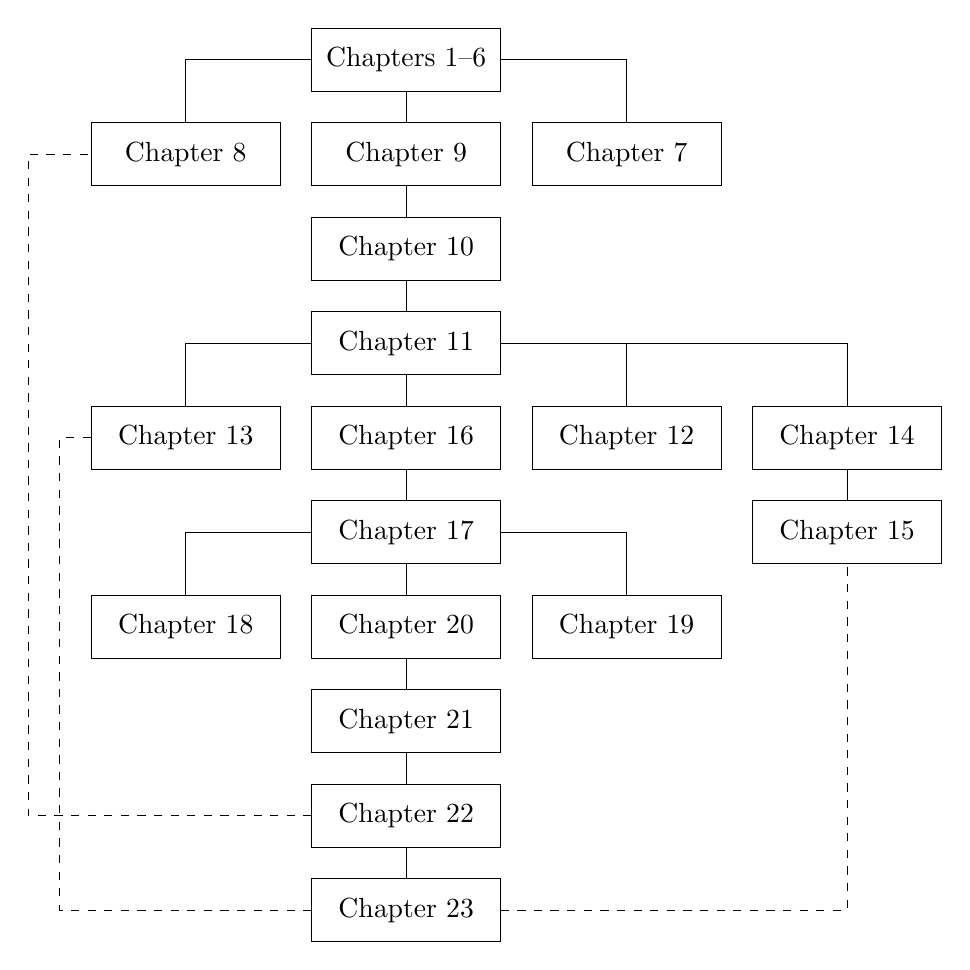
\begin{tikzpicture}[scale=0.8]  %Replaced figure with tikz figure - TWJ 6/14/2010

\draw (3.5,0) rectangle (6.5,1);
\node at (5,0.5) {Chapter 23};

\draw (3.5,1.5) rectangle (6.5,2.5);
\node at (5,2) {Chapter 22};

\draw (3.5,3) rectangle (6.5,4);
\node at (5,3.5) {Chapter 21};

\draw (0,4.5) rectangle (3,5.5);
\node at (1.5,5) {Chapter 18};

\draw (3.5,4.5) rectangle (6.5,5.5);
\node at (5,5) {Chapter 20};

\draw (7,4.5) rectangle (10,5.5);
\node at (8.5,5) {Chapter 19};

\draw (3.5,6) rectangle (6.5,7);
\node at (5,6.5) {Chapter 17};

\draw (10.5,6) rectangle (13.5,7);
\node at (12,6.5) {Chapter 15};

\draw (0,7.5) rectangle (3,8.5);
\node at (1.5,8) {Chapter 13};

\draw (3.5,7.5) rectangle (6.5,8.5);
\node at (5,8) {Chapter 16};

\draw (7,7.5) rectangle (10,8.5);
\node at (8.5,8) {Chapter 12};

\draw (10.5,7.5) rectangle (13.5,8.5);
\node at (12,8) {Chapter 14};

\draw (3.5,9) rectangle (6.5,10);
\node at (5,9.5) {Chapter 11};

\draw (3.5,10.5) rectangle (6.5,11.5);
\node at (5,11) {Chapter 10};

\draw (0,12) rectangle (3,13);
\node at (1.5,12.5) {Chapter 8};

\draw (3.5,12) rectangle (6.5,13);
\node at (5,12.5) {Chapter 9};

\draw (7,12) rectangle (10,13);
\node at (8.5,12.5) {Chapter 7};

\draw (3.5,13.5) rectangle (6.5,14.5);
\node at (5,14) {Chapters 1--6};

\draw (5,1) -- (5,1.5) (5,2.5) -- (5,3)  (5,4) -- (5,4.5)  (5,5.5) -- (5,6)  (5,7) -- (5,7.5)  (5,8.5) -- (5,9)  (5,10) -- (5,10.5)  (5,11.5) -- (5,12)  (5,13) -- (5,13.5);

\draw [dashed] (6.5,0.5) -- (12,0.5) -- (12,6);

\draw (12,7) -- (12,7.5) (12,8.5) -- (12,9.5) -- (6.5,9.5) (8.5,8.5) -- (8.5,9.5);

\draw (8.5,5.5) -- (8.5,6.5) -- (6.5,6.5);

\draw (8.5,13) -- (8.5,14) -- (6.5,14);

\draw [dashed] (3.5,0.5) -- (-0.5,0.5) -- (-0.5,8) -- (0,8);

\draw [dashed] (3.5,2) -- (-1,2) -- (-1,12.5) -- (0,12.5);

\draw (1.5,5.5) -- (1.5,6.5) -- (3.5,6.5);

\draw (1.5,8.5) -- (1.5,9.5) -- (3.5,9.5);

\draw (1.5,13) -- (1.5,14) -- (3.5,14);

\end{tikzpicture}

\end{center}
\end{figure}

Though there are no specific prerequisites for a course in abstract
algebra, students who have had other higher-level courses in
mathematics will generally be more prepared than those who have not,
because they will possess a bit more mathematical sophistication.
Occasionally, we shall assume some basic linear algebra; that is, we
shall take for granted an elementary knowledge of matrices and
determinants. This should present no great problem, since most
students taking a course in abstract algebra have been introduced to
matrices and determinants elsewhere in their career, if they have not
already taken a sophomore- or junior-level course in linear algebra.

Exercise sections are the heart of any mathematics text. An exercise
set appears at the end of each chapter. The nature of the exercises
ranges over several categories; computational,  conceptual, and
theoretical problems are included. A section presenting hints and
solutions to many of the exercises appears at the end of the text.
Often in the solutions a proof is only sketched, and it is up to the
student to provide the details. The exercises range in difficulty from
very easy to very challenging. Many of the more substantial problems
require careful thought, so the student should not be discouraged if
the solution is not forthcoming after a few minutes of work. 
% A complete solutions manual is available for the instructor's use. 
% Removed reference to the solutions manual.  TWJ 8/19/2010

There are additional exercises or computer projects at the ends of
many of the chapters. The computer projects usually require a
knowledge of programming. All of these exercises and projects are more
substantial in nature and allow the exploration of new results and
theory.

% Added Sage blurb, RAB 2011/07/28
Sage (\url{sagemath.org}) is a free, open source, software system
for advanced mathematics, which is ideal for assisting with a study
of abstract algebra. Comprehensive discussion about Sage, and a
selection of relevant exercises, are provided in an electronic
format that may be used with the Sage Notebook in a web browser,
either on your own computer, or at a public server such as
\url{sagenb.org}.  Look for this supplement at the book's
website: \url{abstract.pugetsound.edu}.  In printed
versions of the book, we include a brief description of Sage's
capabilities at the end of each chapter, right after the references.

The open source version of this book has received support from the National Science Foundation (Award \# 1020957).
%Added NSF support statement.  TWJ 8/9/2012

\section*{Acknowledgements}

I would like to acknowledge the following reviewers for their helpful
comments and suggestions. 
\begin{itemize}
 
\item
David Anderson,
University of Tennessee, Knoxville

\item
Robert Beezer,
University of Puget Sound

\item
Myron Hood,
California Polytechnic State University

\item
Herbert Kasube,
Bradley University

\item
John Kurtzke,
University of Portland
 
\item
Inessa Levi,
University of Louisville
 
\item
Geoffrey Mason,
University of California, Santa Cruz

\item
Bruce Mericle,
Mankato State University
 
\item
Kimmo Rosenthal,
Union College

\item
Mark Teply,
University of Wisconsin

\end{itemize}
I would also like to thank Steve Quigley, Marnie Pommett, Cathie
Griffin, Kelle Karshick, and the rest of the staff at PWS for their
guidance throughout this project. It has been a pleasure to work with
them. 

 
\begin{flushright}
Thomas W. Judson
\end{flushright}
 
 
\pagestyle{headings}
 
 
 
 


\tableofcontents



%**********************included files************************ 

\cleardoublepage 
\setcounter{chapter}{-1}
\pagenumbering{arabic}


%%%%(c)
%%%%(c)  This file is a portion of the source for the textbook
%%%%(c)
%%%%(c)    Abstract Algebra: Theory and Applications
%%%%(c)    by Thomas W. Judson
%%%%(c)
%%%%(c)    Sage Material
%%%%(c)    Copyright 2011 by Robert A. Beezer
%%%%(c)
%%%%(c)  See the file COPYING.txt for copying conditions
%%%%(c)
%%%%(c)
\begin{sageverbatim}\end{sageverbatim}
%
\sageexercise{1}%
This exercise is just about making sure you know how to use Sage.  Login to a notebook server and create a new worksheet.  Do some non-trivial computation, maybe a pretty plot or some gruesome numerical computation to an insane precision.   Create an interesting list and experiment with it some.  Maybe include some nicely formatted text or \TeX\ using the included mini-word-processor (hover until a blue bar appears between cells and then shift-click).\par
%
Use whatever mechanism your instructor has in place for submitting your work.  Or save your worksheet and then trade worksheets via email (or another electronic method) with a classmate.
\begin{sageverbatim}\end{sageverbatim}
%
     %Set Theory
Sage's original purpose was to support research in number theory, so it is perfect for the types of computations with the integers that we have in this chapter. %Integers
The first half of this text is about group theory.  Sage includes GAP, a program designed primarly for just group theory, and in continuous development since 1986.  Many of Sage's computations for groups ultimately are performed by GAP.   %Groups
%%%%(c)
%%%%(c)  This file is a portion of the source for the textbook
%%%%(c)
%%%%(c)    Abstract Algebra: Theory and Applications
%%%%(c)    by Thomas W. Judson
%%%%(c)
%%%%(c)    Sage Material
%%%%(c)    Copyright 2011 by Robert A. Beezer
%%%%(c)
%%%%(c)  See the file COPYING.txt for copying conditions
%%%%(c)
%%%%(c)
This group of exercises is about the group of units mod $n$, $U(n)$, which is sometimes cyclic, sometimes not.  There are some commands in Sage that will answer some of these questions very quickly, but instead of using those now, just use the basic techniques described.  The idea here is to just work with elements, and lists of elements, to discern the subgroup structure of these groups.\par
\begin{sageverbatim}\end{sageverbatim}
%
\sageexercise{1}%
Execute the statement \verb?U = Integers(40)? to create the set \verb?[0,1,2,...,39]?  This is a group under addition mod $40$, which we will ignore.  Instead we are interested in the subset of elements which have an inverse under \emph{multiplication} mod $40$.  Determine how big this subgroup is by executing the command \verb?U.unit_group_order()?, and then obtain a list of these elements with \verb?U.list_of_elements_of_multiplicative_group()?.\par
\begin{sageverbatim}\end{sageverbatim}
%
\sageexercise{2}%
You can create elements of this group by coercing regular integers into \verb?U?, such as  with the statement \verb?a = U(7)?.  (Don't confuse this with our mathematical notation $U(40)$.)  This will tell Sage that you want to view $7$ as an element of $U$, subject to the corresponding operations.  Determine the elements of the cyclic subgroup of $U$ generated by $7$ with a list comprehension as follows:
%
\begin{sageverbatim}
sage: U = Integers(40)
sage: a = U(7)
sage: [a^i for i in range(16)]
\end{sageverbatim}
%
What is the order of $7$ in $U(40)$?\par
\begin{sageverbatim}\end{sageverbatim}
%
\sageexercise{3}%
The group $U(49)$ is cyclic.  Using only the Sage commands described previously, use Sage to find a generator for this group.  Now using \emph{only} theorems about the structure of cyclic groups, describe each of the subgroups of $U(49)$ by specifying its order and by giving an explicit generator.  Do not repeat any of the subgroups --- in other words, present each subgroup \emph{exactly} once.  You can use Sage to check your work on the subgroups, but your answer about the subgroups should rely only on theorems and be a nicely written paragraph with a table, etc.\par
\begin{sageverbatim}\end{sageverbatim}
%
\sageexercise{4}%
The group $U(35)$ is not cyclic.  Again, using only the Sage commands described previously, use computations to provide irrefutable evidence of this.  How many of the 16 different subgroups of $U(35)$ can you list?\par
\begin{sageverbatim}\end{sageverbatim}
%
\sageexercise{5}%
Again, using only the Sage commands described previously, explore the structure of $U(n)$ for various values of $n$ and see if you can formulate an interesting conjecture about some basic property of this group.  (Yes, this is a {\em very} open-ended question, but this is ultimately the real power of exploring mathematics with Sage.)
\begin{sageverbatim}\end{sageverbatim}
%
   %Cyclic Groups
%%%%(c)
%%%%(c)  This file is a portion of the source for the textbook
%%%%(c)
%%%%(c)    Abstract Algebra: Theory and Applications
%%%%(c)    by Thomas W. Judson
%%%%(c)
%%%%(c)    Sage Material
%%%%(c)    Copyright 2011 by Robert A. Beezer
%%%%(c)
%%%%(c)  See the file COPYING.txt for copying conditions
%%%%(c)
%%%%(c)
These exercises are designed to help you become familiar with permutation groups in Sage.
%
\begin{sageverbatim}\end{sageverbatim}
%
\sageexercise{1}%
Create the full symmetric group $S_{10}$ with the command \verb?G = SymmetricGroup(10)?.
\begin{sageverbatim}\end{sageverbatim}
%
\sageexercise{2}
Create elements of \verb?G? with the following (varying) syntax.  Pay attention to commas, quotes, brackets, parentheses.  The first two use a string (characters) as input, mimicking the way we write permuations (but with commas).  The second two use a list of tuples.\par\noindent
(a) \verb?a = G("(5,7,2,9,3,1,8)")?\\
(b) \verb?b = G("(1,3)(4,5)")?\\
(c) \verb?c = G([(1,2),(3,4)])?\\
(d) \verb?d = G([(1,3),(2,5,8),(4,6,7,9,10)])?
\begin{sageverbatim}\end{sageverbatim}
%
\sageexercise{3}
%
Compute $a^3$, $bc$, $ad^{-1}b$.
\begin{sageverbatim}\end{sageverbatim}
%
\sageexercise{4}
%
Compute the orders of each of these four individual elements (\verb?a? through \verb?d?) using a single permutation group element method.
\begin{sageverbatim}\end{sageverbatim}
%
\sageexercise{5}
Use the permutation group element method \verb?.sign()? to determine if $a,b,c,d$ are even or odd permutations.
\begin{sageverbatim}\end{sageverbatim}
%
\sageexercise{6}
Create two cyclic subgroups of $G$ with the commands:
%
\begin{itemize}
\item\verb?H = G.subgroup([a])?
\item\verb?K = G.subgroup([d])?
\end{itemize}
%
List, and study, the elements of each subgroup.  List the size and number of all of the subgroups of $K$ (without using Sage), and construct a subgroup of $K$ of size 10 using Sage.
\begin{sageverbatim}\end{sageverbatim}
%
\sageexercise{7}
More complicated subgroups can be formed by using two or more generators.  Construct a subgroup $L$ of $G$ with the command \verb?L = G.subgroup([b,c])?.  Compute the order of $L$ and list all of the elements of $L$.
\begin{sageverbatim}\end{sageverbatim}
%
\sageexercise{8}
Construct the group of symmetries of the tetrahedron (also the alternating group on 4 symbols, $A_4$) with the command \verb?A=AlternatingGroup(4)?.  Using tools such as orders of elements, and generators of subgroups, see if you can find \emph{all of} the subgroups of $A_4$ (each one exactly once).  Provide a nice summary as your answer - not just piles of output.  So use Sage as a tool, as needed, but basically your answer will be a concise paragraph and/or table.  This is the one part of this assignment without clear, precise directions, so spend some time on this portion to get it right.  Hint: no subgroup of $A_4$ requires more than two generators.
\begin{sageverbatim}\end{sageverbatim}
%
\sageexercise{9}
Save your work, and then see if you can crash your Sage session with the commands:
%
\begin{itemize}
\item\verb?N = G.subgroup([b,d])?
\item\verb?N.list()?
\end{itemize}
%
How big is $N$?
\begin{sageverbatim}\end{sageverbatim}
%
\sageexercise{10}
Answer the five questions above about the permutations of the cube expressed as permutations of the 8 vertices.
\begin{sageverbatim}\end{sageverbatim}
%
  %Permutation Groups
The following exercises are less about cosets and subgroups, and more about using Sage as an experimental tool.  We will have many opportunities to work with cosets and subgroups in the coming chapters.\par
%
These exercises do not contain much guidance, and get more challenging as they go.  They are designed to explore, or confirm, results presented in this chapter.  Generally, they can be each be answered with a single (complicated) line of Sage that concludes by outputting \verb?True?.
\begin{sageverbatim}\end{sageverbatim}
%
\sageexercise{1}%
Use \verb?.subgroups()? to find an example of a group $G$ and an integer $m$, so that (a) $m$ divides the order of $G$, and (b) $G$ has no subgroup of order $m$.  (Do not use the group $A_4$ for $G$, since this is in the text.)  Provide just enough output to convince the reader that your example is correct.  Here is a very simple example that might help you structure the logic of a one-line verification.
%
\begin{sageexample}
sage: a = 5
sage: b = 10
sage: c = 6
sage: d = 13
sage: a.divides(b)
True
sage: not (b in [c,d])
True
sage: a.divides(b) and not (b in [c,d])
True
\end{sageexample}
%
\begin{sageverbatim}\end{sageverbatim}
%
\sageexercise{2}%
Verify the truth of Fermat's Little Theorem (either variant) for your own choice of a single number for the base $a$ (or $b$), and for $p$ assuming the value of every prime number between $100$ and $1000$.  Build up a solution slowly --- make a list of powers (start with just a few primes), then make a list of powers reduced by modular arithmetic, then a list of comparisons with  the predicted value, then a check on all these logical values resulting from the comparisons.  Eventually you can write a single line that performs the verification by eventually printing out \verb?True?.  Some more hints about useful functions follow below.
%
\begin{sageexample}
sage: a = 20
sage: b = 6
sage: a.mod(b)
2
sage: prime_range(50, 100)
[53, 59, 61, 67, 71, 73, 79, 83, 89, 97]
sage: all([True, True, True, True])
True
sage: all([True, True, False, True])
False
\end{sageexample}
%
\begin{sageverbatim}\end{sageverbatim}
%
\sageexercise{3}%
Verify that the group of units mod $n$ has order $n-1$ when $n$ is prime, again for all primes between $100$ and $1000$.  As before, your output should be simply \verb?True?, just once indicating that the statement about the order is true for all the primes examined.  As before, build up your solution slowly, and with a smaller range of primes in the beginning.
\begin{sageverbatim}\end{sageverbatim}
%
\sageexercise{4}%
Verify Euler's Theorem for all values of $n<100$ and for $a \leq n$.  This will require nested \verb?for? statements with a conditional.  Again, here's a small example that might be helpful.
%
\begin{sageexample}
sage: [a/b for a in srange(9) for b in srange(1,a) if gcd(a,b)==1]
[2, 3, 3/2, 4, 4/3, 5, 5/2, 5/3, 5/4, 6, 6/5,
 7, 7/2, 7/3, 7/4, 7/5, 7/6, 8, 8/3, 8/5, 8/7]
\end{sageexample}
%
\begin{sageverbatim}\end{sageverbatim}
%

   %Cosets and Lagrange's Theorem
%%%%(c)
%%%%(c)  This file is a portion of the source for the textbook
%%%%(c)
%%%%(c)    Abstract Algebra: Theory and Applications
%%%%(c)    Copyright 1997 by Thomas W. Judson
%%%%(c)
%%%%(c)  See the file COPYING.txt for copying conditions
%%%%(c)
%%%%(c)
\chap{Introduction to Cryptography}{crypt}

Cryptography is the study of sending and receiving secret messages.
The aim of cryptography is to send messages across a channel so only
the intended recipient of the message can read it. In addition, when a
message is received, the recipient usually requires some assurance that
the message is authentic; that is, that it has not been sent by
someone who is trying to deceive the recipient. Modern cryptography is
heavily dependent on abstract algebra and number theory. 
 
 
The message to be sent is called the \boldemph{
plaintext}\index{Plaintext} message. The disguised message is called
the \boldemph{ciphertext}\index{Ciphertext}. The plaintext and the
ciphertext are both written in an \boldemph{alphabet}, consisting of \boldemph{
letters} or \boldemph{characters}. Characters can include not only the
familiar alphabetic characters A, $\ldots$, Z and a, $\ldots$, z but
also digits, punctuation marks, and blanks. A \boldemph{
cryptosystem},\index{Cryptosystem!definition of} or \boldemph{
cipher},\index{Cipher}  has two parts: \boldemph{encryption}, the process
of transforming a plaintext message to a ciphertext message, and \boldemph{
decryption}, the reverse transformation of changing a ciphertext
message into a plaintext message.
 
 
There are many different families of cryptosystems, each distinguished
by a particular encryption algorithm. Cryptosystems in a specified
cryptographic family are distinguished from one another by a parameter
to the encryption function called a \boldemph{key}\index{Key!definition
of}. A classical cryptosystem has a single key, which must be kept
secret,  known only to the sender and the receiver of the message. If
person $A$ wishes to send secret messages to two different people $B$
and $C$, and does not wish to have $B$ understand $C$'s messages or
vice versa, $A$ must use two separate keys, so one cryptosystem is
used for exchanging messages with $B$, and another is used for
exchanging messages with $C$.
 
 
Systems that use two separate keys, one for encoding and another for
decoding, are called \boldemph{public key
cryptosystems}\index{Key!public}\index{Cryptosystem!public key}. Since
knowledge of the encoding key does not allow anyone to guess at the
decoding key, the encoding key can be made public. A public key
cryptosystem allows $A$ and $B$ to send messages to $C$ using the same
encoding key.  Anyone is capable of encoding a message to be sent to
$C$, but only $C$ knows how to decode such a message.
 

\section{Private Key Cryptography}
 
In \boldemph{single}\index{Key!single}\index{Cryptosystem!single key} or
\boldemph{private key
cryptosystems}\index{Key!private}\index{Cryptosystem!private key}
the same key is used for both encrypting and decrypting messages. To
encrypt a  plaintext message, we apply to the message some function
which is kept secret, say $f$. This function will yield an encrypted
message.  Given the encrypted form of the message, we can recover the
original message by applying the inverse transformation $f^{-1}$. The
transformation $f$ must be relatively easy to compute, as must
$f^{-1}$; however, $f$ must be extremely difficult to guess at if only
examples of coded messages are available.
 
\begin{example}{caesar}
One of the first and most famous private key cryptosystems was the
shift code used by Julius Caesar.  We first digitize the alphabet by
letting $\mbox{A}  = 00, \mbox{B}  = 01, \ldots, \mbox{Z} = 25$.
The encoding function will be 
\[
f(p) = p + 3 \bmod 26;
\]
that is, $A \mapsto D, B \mapsto E, \ldots, Z \mapsto C$. The decoding
function is then 
\[
f^{-1}(p) = p - 3 \bmod 26 = p + 23 \bmod 26.
\]
Suppose we receive the encoded message DOJHEUD. To decode this
message, we first digitize it:  
\[
3, 14, 9, 7, 4, 20, 3.
\]
Next we apply the inverse transformation to get
\[
0, 11, 6, 4, 1, 17, 0,
\]
or ALGEBRA. Notice here that there is nothing special about either of
the numbers 3 or 26. We could have used a larger alphabet or a
different shift.
\mbox{\hspace{1in}}
\end{example}

 
\boldemph{Cryptanalysis}\index{Cryptanalysis} is concerned with
deciphering a received or intercepted message. Methods from
probability and statistics are great aids in deciphering an
intercepted message; for example, the frequency analysis of the
characters appearing in the intercepted message often makes its
decryption possible.  
 
 
\begin{example}{crypt_analysis}
Suppose we receive a message that we know was encrypted by using a
shift transformation on single letters of the 26-letter alphabet. To
find out exactly what the shift transformation was, we must compute
$b$ in the equation $f(p) = p + b \bmod 26$. We can do this using
frequency analysis.  The letter $\mbox{E} = 04$ is the most commonly
occurring letter in the English language. Suppose that $\mbox{S} = 18$
is the most commonly occurring letter in the ciphertext.  Then we have
good reason to suspect that  $18 = 4 + b \bmod 26$, or $b= 14$.
Therefore, the most likely encrypting function is
\[
f(p) = p + 14 \bmod 26.
\]
The corresponding decrypting function is
\[
f^{-1}(p) = p + 12 \bmod 26.
\]
It is now easy to determine whether or not our guess is correct.
\end{example}
 
 
Simple shift codes are examples of \boldemph{monoalphabetic
cryptosystems}\index{Cryptosystem!monoalphabetic}. In these ciphers a
character in the enciphered message represents exactly one character
in the original message. Such cryptosystems are not very sophisticated
and are quite easy to break. In fact, in a simple shift as described
in Example~\ref{example:crypt:caesar}, there are only 26 possible keys. It would be quite easy
to try them all rather than to use frequency analysis. 
 
 
Let us investigate a slightly more sophisticated cryptosystem. Suppose
that the encoding function is given by  
\[
f(p) = ap + b \bmod 26.
\]
We first need to find out when a decoding function $f^{-1}$ exists.
Such a decoding function exists when we can solve the equation
\[
c = ap + b \bmod 26
\]
for $p$. By Proposition~\ref{Zn_equiv_classes}, this is possible exactly when $a$ has an
inverse or, equivalently, when $\gcd( a, 26) =1$. In this case 
\[
f^{-1}(p) = a^{-1} p - a^{-1} b \bmod 26.
\]
Such a cryptosystem is called an \boldemph{affine
cryptosystem}\index{Cryptosystem!affine}. 
 
 
\begin{example}{affine_crypt}
Let us consider the affine cryptosystem $f(p) = ap + b \bmod 26$. For
this cryptosystem to work we must choose an $a \in {\mathbb Z}_{26}$
that is invertible. This is only possible if $\gcd(a, 26) = 1$.
Recognizing this fact, we will let $a = 5$ since $\gcd(5, 26) = 1$. It
is easy to see that $a^{-1} = 21$. Therefore, we can take our
encryption function to be $f(p) = 5p + 3 \bmod 26$. Thus, ALGEBRA is
encoded as $3, 6, 7, 23, 8, 10, 3$, or DGHXIKD. The decryption
function will~be   
\[
f^{-1}(p) = 21 p - 21 \cdot 3 \bmod 26 = 21 p + 15 \bmod 26.
\]
\end{example} 
 
A cryptosystem would be more secure if a ciphertext letter could
represent more than one plaintext letter.  To give an example of this
type of cryptosystem, called a \boldemph{polyalphabetic
cryptosystem},\index{Cryptosystem!polyalphabetic} we will generalize
affine codes by using matrices. The idea works roughly the same as
before; however, instead of encrypting one letter at a time we will
encrypt pairs of letters.  We can store a pair of letters $p_1$ and
$p_2$ in a vector  
\[
{\mathbf p} = 
\begin{pmatrix}
p_1 \\ p_2
\end{pmatrix}.
\]
Let $A$ be a $2 \times 2$ invertible matrix
with entries in ${\mathbb Z}_{26}$. We can define an encoding function by
\[
f({\mathbf p}) = A {\mathbf p} + {\mathbf b} ,
\]
where ${\mathbf b}$ is a fixed column vector and matrix operations are
performed in ${\mathbb Z}_{26}$. The decoding function must be
\[
f^{-1}({\mathbf p}) = A^{-1} {\mathbf p} - A^{-1} {\mathbf b}.
\]
 
 
\begin{example}{HELP}
Suppose that we wish to encode the word HELP. The corresponding
digit string is $7, 4, 11, 15$. If
\[
A =
\begin{pmatrix}
3 & 5 \\
1 & 2
\end{pmatrix},
\]
then
\[
A^{-1} 
=
\begin{pmatrix}
2 & 21 \\
25 & 3
\end{pmatrix}.
\]
If ${\mathbf b} = ( 2, 2)^{\rm t}$, then our message is encrypted as
RRCR. The encrypted letter R represents more than one plaintext
letter. 
\end{example}
 
 
Frequency analysis can still be performed on a polyalphabetic
cryptosystem, because we have a good understanding of how pairs of
letters appear in the English language. The pair \emph{th} appears
quite often; the pair \emph{qz} never appears.  To avoid decryption by
a third party, we must use a larger matrix than the one we used in
Example~\ref{example:crypt:HELP}. 

%TWJ 4/7/2010 Need to resolve this reference

  
 
 
\section{Public Key Cryptography}
 
 
 
If traditional cryptosystems are used, anyone who knows enough to
encode a message will also know enough to decode an intercepted
message. In 1976, W.~Diffie\index{Diffie, W.} and
M.~Hellman\index{Hellman, M.} proposed public key cryptography, which
is based on the observation that the encryption and decryption
procedures need not have the same key. This removes the requirement
that the encoding key be kept secret. The encoding function $f$ must
be relatively easy to compute, but $f^{-1}$ must be extremely
difficult to compute without some additional information, so that
someone who knows only the encrypting key cannot find the decrypting
key without prohibitive computation. It is interesting to note that to
date, no system has been proposed that has been proven to be
``one-way;'' that is, for any existing public key cryptosystem, it has
never been shown to be computationally prohibitive to decode messages
with only knowledge of the encoding key. 
 
 
 
\subsection*{The RSA Cryptosystem}
 
The RSA cryptosystem introduced by R.~Rivest\index{Rivest, R.},
A.~Shamir\index{Shamir, A.}, and L.~Adleman\index{Adleman, L.} in
1978, is based on the difficulty of factoring large numbers. Though it
is not a difficult task to find two large random primes and multiply
them together, factoring a 150-digit number that is the product of two
large primes would take 100 million computers operating at 10 million
instructions per second about 50 million years under the fastest
algorithms currently known.
 
 
The RSA cryptosystem\index{RSA cryptosystem}\index{Cryptosystem!RSA}
works as follows. Suppose that we choose two random 150-digit prime
numbers $p$ and $q$. Next, we compute the product $n= pq$ and also
compute $\phi(n) = m = (p - 1)(q-1)$, where $\phi$ is the Euler
$\phi$-function.  Now we start choosing random integers $E$ until we
find one that is relatively prime to $m$; that is, we choose $E$ such
that $\gcd(E, m) = 1$. Using the Euclidean algorithm, we can find a
number $D$ such that \mbox{$DE \equiv 1 \pmod{m}$}. The numbers $n$ and $E$
are now made public. 
 
 
Suppose now that person B (Bob) wishes to send person A (Alice) a
message over a public line. Since $E$ and $n$ are known to everyone,
anyone can encode messages. Bob first digitizes the message according
to some scheme, say $\mbox{A}  = 00, \mbox{B}  = 02, \ldots, \mbox{Z}=
25$. If necessary, he will break the message into pieces such that
each piece is a positive integer less than $n$.  Suppose $x$ is one of
the pieces.  Bob forms the number $y = x^E \mod n$ and sends $y$ to
Alice. For Alice to recover $x$, she need only compute $x = y^D \bmod
n$. Only Alice knows $D$.  
 
 
\begin{example}{RSA}
Before exploring the theory behind the RSA cryptosystem or attempting
to use large integers, we will use some small integers just to see
that the system does indeed work. Suppose that we wish to send some
message, which when digitized is 25. Let $p = 23$ and $q = 29$. Then 
\[
n = pq = 667
\]
and
\[
\phi(n) = m = (p - 1)(q - 1) = 616.
\]
We can let $E = 487$, since $\gcd(616, 487) = 1$. The encoded message
is computed to be  
\[
25^{487} \bmod 667 = 169.
\]
This computation can be reasonably done by using the method of
repeated squares as described in Chapter~\ref{cyclic}. Using the Euclidean
algorithm, we determine that $191 E = 1 + 151 m$; therefore, the
decrypting key is $(n, D) = ( 667, 191)$. We can recover the original 
message by calculating  
\[
169^{191} \bmod 667 = 25.
\]
\end{example}

%Message changed from 23 to 25 so that it does not match p.  Suggested by R. Beezer.
%TWJ - 12/19/2011
 
Now let us examine why the RSA cryptosystem works.  We know that $DE
\equiv 1 \pmod{ m}$; hence, there exists a $k$ such that 
\[
DE = km + 1 = k \phi(n) + 1.
\]
There are two cases to consider.  In the first case assume that $\gcd(x, n) = 1$.  Then by Theorem~\ref{cosets:Eulers_theorem},
\[
y^D = (x^E)^D = x^{DE} = x^{km+1} = (x^{\phi(n)})^k x
= (1)^k x= x \bmod n.
\]
So we see that Alice recovers the original message $x$ when
she computes $y^D \bmod n$.

For the other case, assume that $\gcd(x, n) \neq 1$.  Since
$n=pq$ and $x < n$, we know $x$ is a multiple of $p$ or a multiple
of $q$, but not both.  We will describe the first possibility only,
since the second is entirely similar.  There is then an integer $r$,
with $r < q$ and $x=rp$.  Note that we have $\gcd(x, q) = 1$
and that $m=\phi(n)=(p-1)(q-1)=\phi(p)\phi(q)$.  Then, using
Theorem~\ref{cosets:Eulers_theorem}, but now mod $q$,
\[
x^{km} = x^{k\phi(p)\phi(q)} = (x^{\phi(q)})^{k\phi(p)}
= (1)^{k\phi(p)} = 1 \bmod q.
\]
So there is an integer $t$ such that $x^{km}=1 + tq$.
Thus, Alice also recovers the message in this case,
\[
y^D = x^{km+1} = x^{km} x = (1+tq) x
= x + tq(rp) = x + trn = x \bmod n.
\]

%Demonstration expanded to two cases.  Suggested by Kevin Halasz.
%RAB - 12/30/2011

We can now ask how one would go about breaking the RSA cryptosystem.
To find $D$ given $n$ and $E$, we simply need to factor $n$ and solve
for $D$ by using the Euclidean algorithm. If we had known that $667 =
23 \cdot 29$ in Example~\ref{example:crypt:RSA}, we could have recovered $D$.    
 
 
 
\subsection*{Message Verification}
 
 
There is a problem of message verification in public key
cryptosystems. Since the encoding key is public knowledge, anyone has
the ability to send an encoded message.  If Alice receives a message
from Bob, she would like to be able to verify that it was Bob who
actually sent the message. Suppose that Bob's encrypting key is $(n',
E')$ and his decrypting key is $(n', D')$.  Also, suppose that Alice's
encrypting key is $(n, E)$ and her decrypting key is $(n, D)$.  Since
encryption keys are public information, they can exchange coded
messages at their convenience.  Bob wishes to assure Alice that the
message he is sending is authentic. Before Bob sends the message $x$
to Alice, he decrypts  $x$ with his own key:
\[
x' = x ^{D'} \bmod n'.
\]
Anyone can change $x'$ back to $x$ just by encryption, but only Bob
has the ability to form $x'$. Now Bob encrypts $x'$ with Alice's
encryption key to form 
\[
y' = {x'}^E  \bmod n,
\]
a message that only Alice can decode.  Alice decodes the message and
then encodes the result with Bob's key to read the original message, a
message that could have only been sent by Bob.
 
 
 
\histhead
 
 
\noindent{\small \histf
Encrypting secret messages goes as far back as ancient Greece and
Rome. As we know, Julius Caesar used a simple shift code to send and
receive messages. However, the formal study of  encoding and decoding
messages probably began with the Arabs in the 1400s. In the fifteenth
and sixteenth centuries mathematicians such as Alberti and Viete
discovered 
that monoalphabetic cryptosystems offered no real security. In the
1800s, F. W. Kasiski established methods for breaking ciphers in
which a ciphertext letter can represent more than one plaintext
letter, if the same key was used several times. This discovery led to
the use of cryptosystems with keys that were used only a single time.
Cryptography was placed on firm mathematical foundations by such people
as W. Friedman and L. Hill in the early part of the twentieth century.
 
 
During World War II mathematicians were very active in cryptography.
Efforts to penetrate the cryptosystems of the Axis nations were 
organized in England and in the United States by such notable
mathematicians as Alan Turing and A. A. Albert. The period after
World War I saw the development of special-purpose machines for
encrypting and decrypting messages. The Allies gained a 
tremendous advantage in World War II by breaking the ciphers produced by 
the German Enigma machine and the Japanese Purple ciphers.
 
 
By the 1970s, interest in commercial cryptography had begun to take
hold. There was a growing need to protect banking transactions,
computer data, and electronic mail. In the early 1970s, IBM developed
and implemented LUZIFER, the forerunner  of the National Bureau of
Standards' Data Encryption Standard (DES). 
 
 
The concept of a public key cryptosystem, due to Diffie and Hellman,
is very recent (1976). It was further developed by Rivest,  
Shamir, and Adleman with the RSA cryptosystem (1978). It is not known
how secure any of these systems are. The trapdoor knapsack
cryptosystem, developed by Merkle and Hellman, has been broken. It is
still an open question whether or not the RSA system can be broken. At
the time of the writing of this book, the largest number factored is
135 digits long, and at the present moment a code is considered secure if
the key is about 400 digits long and is the product of two 200-digit primes.
There has been a great deal of controversy about research in
cryptography in recent times: the National Security Agency would like to
keep information about cryptography secret, whereas the academic community
has fought for the right to publish basic research.   
 
 
Modern cryptography has come a long way since 1929, when Henry Stimson, 
Secretary of State under Herbert Hoover, dismissed the Black Chamber
(the State Department's cryptography division) in 1929 on the ethical 
grounds that ``gentlemen do not read each other's mail.''
\histbox
}
 
 
 
\markright{EXERCISES}
\section*{Exercises}
\exrule
 
 
{\small 
\begin{enumerate}
 
\item
Encode IXLOVEXMATH using the cryptosystem in Example~\ref{example:crypt:caesar}.
 
\item
Decode ZLOOA WKLVA EHARQ WKHA ILQDO, which was encoded using the
cryptosystem in Example~\ref{example:crypt:caesar}. 
 
 
\item
Assuming that monoalphabetic code was used to encode the following
secret message, what was the original message?
\begin{center}
NBQFRSMXZF YAWJUFHWFF ESKGQCFWDQ AFNBQFTILO FCWP
\end{center}
 
 
 
\item
What is the total number of possible monoalphabetic cryptosystems? How 
secure are such cryptosystems?
 
 
\item
Prove that a $2 \times 2$ matrix $A$ with entries in ${\mathbb Z}_{26}$
is invertible if and only if $\gcd( \det(A), 26 ) = 1$.
 
 
 
\item
Given the matrix 
\[
A =
\begin{pmatrix}
3 & 4 \\
2 & 3
\end{pmatrix},
\]
use the encryption function $f({\mathbf p}) = A {\mathbf p} + {\mathbf b}$
to encode the message CRYPTOLOGY, where ${\mathbf b} = ( 2, 5)^{\rm
t}$.  What is the decoding function?  
 
 
\item\label{RSA_Exercise}
Encrypt each of the following RSA messages $x$ so that $x$ is divided
into blocks of integers of length 2;  that is, if $x = 142528$, encode 
14, 25, and 28 separately.
\begin{enumerate}
 
 
\item
$n = 3551, E = 629, x = 31$
 
\item
$n = 2257, E = 47, x = 23$

\item
$n = 120979, E = 13251, x = 142371$
 
\item
$n = 45629, E = 781, x = 231561$
 

 \end{enumerate}

 
 
\item
Compute the decoding key $D$ for each of the encoding keys in
Exercise~\ref{RSA_Exercise}. 
 
 
\item
Decrypt each of the following RSA messages $y$.
\begin{enumerate}
 
 
\item
$n = 3551, D = 1997, y = 2791$

\item
$n = 5893, D = 81, y = 34$
 
\item
$n = 120979, D = 27331, y = 112135$
 
\item
$n = 79403, D = 671, y = 129381$
 
\end{enumerate}

 

 
\item
For each of the following encryption keys $(n, E)$ in the RSA
cryptosystem, compute $D$.
\begin{enumerate}
 
 \item
$(n, E) = (451, 231)$

 
 \item
$(n, E) = (3053, 1921)$
 
 \item
$(n, E) = (37986733, 12371)$
 
 \item
$(n, E) = (16394854313, 34578451)$
 
\end{enumerate}

 
 
  
 
\item
Encrypted messages are often divided into blocks of $n$ letters. A
message such as THE WORLD WONDERS WHY might be encrypted as 
JIW OCFRJ LPOEVYQ IOC but sent as JIW OCF RJL POE VYQ
IOC.  What are the advantages of using blocks of $n$ letters? 
 
 
\item
Find integers $n$, $E$, and $X$ such that
\[
X^E \equiv X \pmod{n}.
\]
Is this a potential problem in the RSA cryptosystem?
 
 
\item
Every person in the class should construct an RSA cryptosystem using primes
that are 10 to 15 digits long.  Hand in $(n, E)$ and an encoded 
message. Keep $D$ secret. See if you can break one another's codes.
 
 
\end{enumerate}
}
 
 
\subsection*{Additional Exercises: Primality and Factoring}
 
{\small 
 
 
In the RSA cryptosystem it is important to be able to find
large prime numbers easily.  Also, this cryptosystem is not secure if we
can factor a composite number that is the product of two large primes.
The solutions to both of these problems are quite easy.  To
find out if a number $n$ is prime or to factor $n$, we can use trial
division. We simply divide $n$ by $d = 2, 3, \ldots, \sqrt{n}$.
Either a factorization will be obtained, or $n$ is prime if no $d$
divides $n$.  The problem is that such a computation is prohibitively
time-consuming if $n$ is very large. 
\begin{enumerate}
 
 
\item
A better algorithm for factoring odd positive integers is \boldemph{
Fermat's factorization algorithm}\index{Fermat's factorization
algorithm}. 
\begin{enumerate}
 
\item
Let $n= ab$ be an odd composite number. Prove that $n$ can be written
as the difference of two perfect squares:
\[
n = x^2 - y^2 = (x-y)(x+y).
\]
Consequently, a positive odd integer can be factored exactly when we
can find integers $x$ and $y$ such that $n = x^2 - y^2$.
 
\item
Write a program to implement the following factorization algorithm
based on the observation in part (a).
 
\medskip
 
{\tt
\begin{tabbing}
xxxx\=xxxx\=xxxx\=xxxx \kill
\> $x \leftarrow \lceil \sqrt{n}\, \rceil$ \\
\> $y \leftarrow 1$ \\
\mbox{\hspace*{1in}} \\
1: \> while $x^2 - y^2 > n$ do \\
\> \> $y \leftarrow y + 1$ \\
\mbox{\hspace*{1in}} \\
\> if $x^2 - y^2 < n$ then \\
\> \>  $x \leftarrow x + 1$ \\
\> \>  $y \leftarrow 1$ \\
\> \>  goto 1 \\
\> else if $x^2 - y^2 = 0$ then \\
\>  \> $a \leftarrow x-y$ \\
\>  \> $b \leftarrow x+y$ \\
\>  \> write $n = a * b$ 
\end{tabbing}
 
}
 
\medskip
 
The expression  $\lceil \sqrt{n}\, \rceil$ means the smallest integer
greater than or equal to the square root of $n$. Write another program
to do factorization using trial division and compare the speed of the
two algorithms. Which algorithm is faster and why?

\end{enumerate}
 
 
\item
\textbf{Primality Testing.}
Recall Fermat's Little Theorem from Chapter~\ref{cosets}. Let $p$ be prime with
$\gcd(a, p) = 1$. Then $a^{p-1} \equiv 1 \pmod{p}$.  We can use
Fermat's Little Theorem as a screening test for primes. For example, 15
cannot be prime since
\[
2^{15-1} \equiv 2^{14} \equiv 4 \pmod{15}.
\]
However, 17 is a potential prime since
\[
2^{17-1} \equiv 2^{16} \equiv 1 \pmod{17}.
\]
We say that an odd composite number $n$ is a \boldemph{
pseudoprime}\index{Pseudoprime} if 
\[
2^{n-1} \equiv 1 \pmod{n}.
\]
Which of the following numbers are primes  and which are pseudoprimes?
\begin{multicols}{3}
\begin{enumerate}

\item
342

\item
811

\item
601

\item
561

\item
771

\item
631
 
\end{enumerate}
\end{multicols}
 
 

\item
Let $n$ be an odd composite number and $b$ be a positive integer such
that $\gcd(b, n) = 1$. If $b^{n-1} \equiv 1 \pmod{n}$, then $n$ is a
\boldemph{pseudoprime base} $b$. Show that 341 is a pseudoprime base 2 but
not a pseudoprime base 3.
 
 
\item
Write a program to determine all primes less than 2000 using
trial division. Write a second program that will determine all numbers
less than 2000 that are either primes or pseudoprimes. Compare the
speed of the two programs.  How many pseudoprimes are there below
2000? 
 
 
There exist composite numbers that are pseudoprimes for all bases to
which they are relatively prime.  These numbers are called \boldemph{
Carmichael numbers}\index{Carmichael numbers}. The first Carmichael
number is $561 = 3 \cdot 11 \cdot 17$.  In 1992, Alford, Granville, and
Pomerance proved that there are an infinite number of Carmichael
numbers [4].  However, Carmichael numbers are very rare.  There are
only $2163$ Carmichael numbers less than $25 \times 10^9$. For more
sophisticated primality tests, see [1], [6], or [7].  
 
 
\end{enumerate}
}
 
 
\subsection*{References and Suggested Readings}
 
{\small
\begin{itemize}
 
\item[\textbf{[1]}]
Bressoud, D. M. \textit{Factorization and Primality Testing}.
Springer-Verlag, New York, 1989. 
 
\item[\textbf{[2]}]
Diffie, W. and Hellman, M. E. ``New Directions in
Cryptography,'' \textit{IEEE Trans. Inform. Theory} \textbf{
22} (1976), 644--54.
 
\item[\textbf{[3]}] %Title corrected.  Suggested by R. Beezer.  TWJ - 12/20/2011
Gardner, M. ``Mathematical games: A new kind of cipher that would take millions
of years to break,'' \textit{Scientific American} \textbf{
237} (1977), 120--24.
 
\item[\textbf{[4]}]%%%%%%%%%%%%%%checked
Granville, A. ``Primality Testing and Carmichael Numbers,'' {\it
Notices of the American Mathematical Society} \textbf{39}(1992),
696--700. 
 
\item[\textbf{[5]}]
Hellman, M. E. ``The Mathematics of Public Key
Cryptography,''  \textit{Scientific American} \textbf{241}
(1979), 130--39.
 

\item[\textbf{[6]}] %reference updated - TWJ 5/10/2010
Koblitz, N. \textit{A Course in Number Theory and Cryptography}. 2nd ed.
Springer, New York, 1994.  
 
 
\item[\textbf{[7]}]
Pomerance, C., ed. \textit{Cryptology and Computational Number
Theory}. Proceedings of Symposia in Applied Mathematics,
vol. 42. American Mathematical Society, Providence, RI,
1990.
 
\item[\textbf{[8]}]
Rivest, R. L., Shamir, A., and Adleman, L., ``A Method for
Obtaining Signatures and Public-key Cryptosystems,'' {\it
Comm. ACM} \textbf{21}(1978), 120--26.
 
\end{itemize}
}
 
\sagesection

 
    %Cryptography
\chapter{Algebraic Coding Theory}
 
 
 
Coding theory is an application of algebra that has become
increasingly important over the last several decades. When we transmit
data, we are concerned about sending a message over a channel that
could be affected by ``noise.'' We wish to be able to encode and
decode the information in a manner that will allow the detection, and
possibly the correction, of errors caused by noise. This situation
arises in many areas of communications, including radio, telephone,
television, computer communications, and even compact disc player
technology. Probability, combinatorics, group theory, linear algebra,
and polynomial rings over finite fields all play important roles in
coding theory.  
 
 
 
\section{Error-Detecting and Correcting Codes}
 
 
Let us examine a simple model of a communications system for
transmitting and receiving coded messages (Figure~\ref{encoding}).  
\begin{figure}[htb]
\begin{center}
\setlength{\unitlength}{.15in}
\begin{picture}(19,23)(0,1)
\thicklines
\put(3.2,1.2){\small \it m-digit received message or error}
\put(5.8,6.3){\small \it n-digit received word}
\put(8.8,11.3){\small \it Noise}
\put(6.7,16.3){\small \it n-digit codeword}
\put(6.7,21.3){\small \it m-digit message}
\put(7,3){\framebox(6,2){\small Decoder}}
\put(7,8){\framebox(6,2){\small Receiver}}
\put(7,13){\framebox(6,2){\small Transmitter}}
\put(7,18){\framebox(6,2){\small Encoder}}
\thinlines
\multiput(10,6)(0,5){4}{\vector(0,-1){1}}
\put(10,3){\vector(0,-1){1}}
\multiput(10,8)(0,5){3}{\line(0,-1){1}}
\end{picture}
\end{center}
\caption{Encoding and decoding messages}
\label{encoding}
\end{figure}
Uncoded messages may be composed of letters or characters, but
typically they consist of binary $m$-tuples. These messages are
encoded into codewords, consisting of binary $n$-tuples, by a device
called an {\bfi encoder}. The message is transmitted and then decoded.
We will consider the occurrence of errors during transmission. An
{\bfi error\/} occurs if there is a change in one or more bits in the
codeword. A {\bfi decoding scheme\/} is a method that either converts
an arbitrarily received $n$-tuple into a meaningful decoded message or
gives an error message for that $n$-tuple. If the received message is
a codeword (one of the special $n$-tuples allowed to be transmitted),
then the decoded message must be the unique message that was encoded
into the codeword. For received noncodewords, the decoding scheme will
give an error indication, or, if we are more clever, will actually try
to correct the error and reconstruct the original message. Our goal is
to transmit error-free messages as cheaply and quickly as possible.
 
 
\vspace{1.5ex}
 
 
\noindent {\bf Example 1.}
One possible coding scheme would be to send a message several
times and to compare the received copies with one another. Suppose
that the message to be encoded is a binary $n$-tuple $(x_{1}, x_{2},
\ldots, x_{n})$. The message is encoded into a binary $3n$-tuple by
simply repeating the message three times: 
\[
(x_{1}, x_{2}, \ldots, x_{n})
\mapsto
(x_{1}, x_{2}, \ldots, x_{n}, x_{1}, x_{2}, \ldots, x_{n},
x_{1}, x_{2}, \ldots, x_{n}).
\]
To decode the message, we choose as the $i$th digit the one that
appears in the $i$th place in at least two of the three transmissions.
For example, if the original message is $(0110)$, then the transmitted
message will be \mbox{$(0110\:0110\:0110)$}. If there is a transmission error
in the fifth digit, then the received codeword will be
$(0110\:1110\:0110)$, which will be correctly decoded as
$(0110)$.\footnote{We will adopt the convention that bits are numbered
left to right in binary $n$-tuples.} 
This triple-repetition method will automatically detect and correct
all single errors, but it is slow and inefficient: to send a message
consisting of $n$ bits, $2n$ extra bits are required, and we can only
detect and correct single errors. We will see that it is possible to
find an encoding scheme that will encode a message of $n$ bits into
$m$ bits with $m$ much smaller than $3n$.
\hspace{\fill} $\blacksquare$
 
 
\vspace{1.5ex}
 
 
\noindent {\bf Example 2.}
{\bfi Even parity}, a  commonly  used coding scheme, is much
more efficient than the simple repetition scheme. The ASCII (American
Standard Code for Information Interchange) coding system uses binary
8-tuples, yielding $2^{8} = 256$ possible 8-tuples. However, only seven
bits are needed since there are only $2^7 = 128$ ASCII characters.
What can or should be done with the extra bit? Using the full eight
bits, we can detect single transmission errors. For example, the ASCII
codes for A, B, and C are 
\[
\begin{array}{rcccl}
\mbox{A} & = & 65_{10} & = & 01000001_{2}, \\
\mbox{B} & = & 66_{10} & = & 01000010_{2}, \\
\mbox{C} & = & 67_{10} & = & 01000011_{2}.
\end{array}
\]
Notice that the leftmost bit is always set to 0; that is, the 128 ASCII
characters have codes 
\begin{eqnarray*}
00000000_{2} & = & 0_{10}, \\
& \vdots & \\
01111111_{2} & = & 127_{10}.
\end{eqnarray*}
The bit can be used for error checking on the other seven bits. It is
set to either 0 or 1 so that the total number of 1 bits in the
representation of a character is even. Using even parity, the codes
for A, B, and C now become 
\begin{eqnarray*}
\mbox{A} & = & 01000001_{2}, \\
\mbox{B} & = & 01000010_{2}, \\
\mbox{C} & = & 11000011_{2}.
\end{eqnarray*}
Suppose an A is sent and a transmission error in the sixth
bit is caused by noise over the communication channel so that 
(01000101) is received. We know an error has occurred since the
received word has an odd number of 1's, and we can now request that the
codeword be transmitted again. When used for error checking, the
leftmost bit is called a {\bfi parity check bit}.  
 
 
By far the most common error-detecting
codes used in computers are based on the addition of a parity bit.
Typically, a computer stores information in $m$-tuples called {\bfi
words}. Common word lengths are 8, 16, and 32 bits. One bit in the 
word is set aside as the parity check bit, and is not used to store
information. This bit is set to either 0 or 1, depending on the
number of 1's in the word. 
 
 
Adding a parity check bit allows the detection of all single errors
because changing a single bit either increases or decreases the number
of 1's by one, and in either case the parity has been changed from
even to odd, so the new word is not a codeword. (We could also
construct an error detection scheme based on {\bfi odd parity}; that
is, we could set the parity check bit so that a codeword always has an
odd number of 1's.)  
\hspace{\fill} $\blacksquare$
 
 
\vspace{1.5ex}
 
 
The even parity system is easy to implement, but has two drawbacks.
First, multiple errors are not detectable. Suppose an A is sent and 
the first and seventh bits are changed from 0 to 1. The received word
is a codeword, but will be decoded into a C instead of an A.
Second, we do not have the ability to correct errors.  If the 8-tuple
(10011000) is received, we know that an error has occurred, but we
have no idea which bit has been changed. We will now investigate a
coding scheme that will not only allow us to detect transmission
errors but will actually correct the errors. 
 
 
\vspace{1.5ex}
 
 
\begin{table}[htb]
\caption{A repetition code}{\small
\begin{center}
\begin{tabular}{|lc|cccccccc|}
\hline
& & \multicolumn{8}{|c|}{Received Word}    \\
            &     & 000 & 001 & 010 & 011 & 100 & 101 & 110
& 111 \\ \hline
Transmitted & 000 & 0   & 1   & 1   & 2   & 1   & 2   & 2
& 3 \\
Codeword   & 111 & 3   &  2  & 2   &  1  &  2  &   1 &  1
&  0 \\ \hline
\end{tabular}
\end{center}
}
\end{table}

 
\noindent {\bf Example 3.}
Suppose that our original message is either a 0 or a 1, and that 0
encodes to (000) and 1 encodes to (111). If only a single
error occurs during transmission, we can detect and correct the
error. For example, if a 101 is received, then the second bit must
have been changed from a 1 to a 0.  The originally transmitted
codeword must have been (111). 	This method will detect and correct 
all single errors. 
 
 
In Table~7.1, we present all possible words that might be received
for the transmitted codewords (000) and (111). Table~7.1 also shows 
the number of bits by which each received 3-tuple differs from each
original codeword. 
\hspace{\fill} $\blacksquare$
 
 
 
\subsection*{Maximum-Likelihood Decoding\footnote{This section
requires a knowledge of probability, but can be
skipped without loss of continuity.}}
 
 
The coding scheme presented in Example~3 is not a complete solution to
the problem because it does not account for the possibility of
multiple errors. For example, either a (000) or a (111) could be sent
and a (001) received. We have no means of deciding from the received
word whether there was a single error in the third bit or two errors,
one in the first bit and one in the second.  No matter what coding 
scheme is used, an incorrect message could
be received: we could transmit a (000), have errors in all three
bits, and receive the codeword (111). It is important to make explicit
assumptions about the likelihood and distribution of transmission
errors so that, in a particular application, it will be known whether
a given
error detection scheme is appropriate. We will assume that
transmission errors are rare, and, that when they do occur, they occur
independently in each bit; that is, if $p$ is the probability of an
error in one bit and $q$ is the probability of an error in a different
bit, then the probability of errors occurring in both of these bits at
the same time is $pq$. We will also assume that a received $n$-tuple 
is
decoded into a codeword that is closest to it; that is, we assume that
the receiver uses {\bfi maximum-likelihood
decoding}\index{Maximum-likelihood decoding}.
 
 
\begin{figure}[htb]
\begin{center}
\setlength{\unitlength}{.1in}
\begin{picture}(14,9)
\put(2,2){\vector(1,0){10}}
\put(2,8){\vector(1,0){10}}
\put(2,2.5){\vector(2,1){10}}
\put(2,7.5){\vector(2,-1){10}}
\put(0.8,7.5){\small 0}
\put(0.8,1.6){\small 1}
\put(12.6,7.5){\small 0}
\put(12.6,1.6){\small 1}
\put(6.5,8.6){\small $p$}
\put(6.5,1){\small $p$}
\put(7.5,6){\small $q$}
\put(7.5,3.5){\small $q$}
\end{picture}
\end{center}
\caption{Binary symmetric channel}
\label{channel}
\end{figure}
 
 
 
A {\bfi binary symmetric channel\/}\index{Binary symmetric channel}
is a model that consists of a transmitter capable of sending a binary 
signal, either a 0 or a 1, together with a receiver. Let $p$ be the 
probability that the signal is correctly
received. Then $q=1-p$ is the probability of an incorrect reception.
If a 1 is sent, then the probability that a 1 is received is $p$ and
the probability that a 0 is received is $q$ (Figure~\ref{channel}).
The probability that no errors occur during the transmission of a binary
codeword of length $n$ is $p^{n}$. For example, if $p=0.999$ and a
message consisting of 10,000 bits is sent, then the probability of a
perfect transmission is 
\[
(0.999)^{10,000} \approx 0.00005.
\]
 
 
\begin{theorem}
If a binary $n$-tuple $(x_{1}, \ldots, x_{n})$ is transmitted across a
binary symmetric channel with probability $p$ that no error will occur
in each coordinate, then the probability that there are errors in
exactly $k$ coordinates~is
\[
\left(
\begin{array}{c}
n \\ k
\end{array}
\right)
 q^kp^{n-k}.
\]
\end{theorem}
 
 
\begin{proof}
Fix $k$ different coordinates. We first compute the probability that
an error has occurred in this fixed set of coordinates. The
probability of an error occurring in a particular one of these $k$
coordinates is $q$; the probability that an error will not occur
in any of the remaining $n-k$ coordinates is $p$. The
probability of each of these $n$ independent events is
$q^{k}p^{n-k}$. The number of possible error patterns with exactly $k$
errors occurring is equal to 
\[
\left(
\begin{array}{c}
n \\ k
\end{array}
\right)
= \frac{n!}{k!(n-k)!},
\]
the number of combinations of $n$ things taken $k$ at a time. Each of
these error patterns has probability $q^{k}p^{n-k}$ of occurring;
hence, the probability of all of these error patterns is
\[
\left(
\begin{array}{c}
n \\ k
\end{array}
\right)
q^{k}p^{n-k}.
\]
\end{proof}
 
 
\vspace{2ex}
 
 
\noindent {\bf Example 4.}
Suppose that $p = 0.995$ and a 500-bit message is sent. The
probability that the message was sent error-free is 
\[
p^{n} = (0.995)^{500} \approx 0.082.
\]
The probability of exactly one error occurring is
\[
\left(
\begin{array}{c}
n \\ 1
\end{array}
\right)
qp^{n-1}= 500(0.005)(0.995)^{499}
\approx 0.204.
\]
The probability of exactly two errors is
\[
\left(
\begin{array}{c}
n \\ 2
\end{array}
\right)
q^{2}p^{n-2}=
\frac{500 \cdot 499}{2}(0.005)^{2}(0.995)^{498} \approx
0.257.
\]
The probability of more than two errors is approximately
\[
1-0.082-0.204 -0.257=0.457.
\]
\hspace{\fill} $\blacksquare$
 
 
\subsection*{Block Codes}
 
 
If we are to develop efficient error-detecting and error-correcting
codes, we will need more sophisticated mathematical tools.  Group
theory  will allow faster methods of encoding and decoding messages. A
code is an $(n, m)$-{\bfi block code\/} if the information that is to be
coded can be divided into blocks of $m$ binary digits, each of which
can be encoded into $n$ binary digits. More specifically, an $(n,
m)$-block code consists of an {\bfi encoding function} 
\[
E:{\Bbb Z}^{m}_{2} \rightarrow {\Bbb Z}^{n}_{2}
\]
and a {\bfi decoding function}
\[
D:{\Bbb Z}^{n}_{2} \rightarrow {\Bbb Z}^{m}_{2}.
\]
A {\bfi codeword\/} is any element in the image of $E$. We also require
that $E$ be one-to-one so that two information blocks will not be
encoded into the same codeword. If our code is to be error-correcting,
then $D$ must be onto.
 
 
\vspace{2ex }
 
 
\noindent {\bf Example 5.}
The even-parity coding system developed to detect single errors in
ASCII characters is an $(8,7)$-block code. The encoding function is
\[
E(x_7, x_6, \ldots, x_1) = (x_8, x_7,  \ldots, x_1),
\]
where $x_8 = x_7 + x_6 + \cdots + x_1$ with addition in ${\Bbb Z}_2$. 
\hspace{\fill} $\blacksquare$
 
 
\vspace{2ex}
 
 
Let ${\bold x} = (x_1, \ldots, x_n)$ and ${\bold y} = (y_1, \ldots,
y_n)$ be binary $n$-tuples. The {\bfi Hamming distance\/}\index{Hamming
distance} or {\bfi distance}, $d({\bold x}, {\bold
y})$\label{noteHammingdist}, between ${\bold x}$ and ${\bold y}$ is
the number of bits in which ${\bold x}$ and ${\bold y}$ differ. The
distance between two codewords is the minimum number of transmission
errors required to change one codeword into the other. The
{\bfi minimum distance\/}\index{Code!minimum distance of} for a code,
$d_{\min}$\label{notemindist}, is the minimum of all distances
$d({\bold x}, {\bold y})$, where ${\bold x}$ and ${\bold y}$ are
distinct codewords. The {\bfi weight}\index{Weight of a codeword},
$w({\bold x})$\label{noteweight}, of a binary codeword ${\bold x}$ is
the number of 1's in ${\bold x}$. Clearly, $w({\bold x}) = d({\bold
x}, {\bold 0})$, where ${\bold 0} = (00 \cdots 0)$. 
 
 
\vspace{2ex}
 
 
\noindent {\bf Example 6.}
Let ${\bold x} = (10101)$, ${\bold y} = (11010)$, and ${\bold z} =
(00011)$ be all of the codewords in some code $C$. Then we have the
following Hamming distances: 
\begin{eqnarray*}
d({\bold x},{\bold y}) & = & 4, \\
d({\bold x},{\bold z}) & = & 3, \\
d({\bold y},{\bold z}) & = & 3.
\end{eqnarray*}
The minimum distance  for this code is 3. We also have the
following weights: 
\begin{eqnarray*}
w({\bold x}) & = & 3, \\
w({\bold y}) & = & 3, \\
w({\bold z}) & = & 2.
\end{eqnarray*}
\hspace{\fill} $\blacksquare$
 
 
\vspace{2ex}
 
 
The following proposition lists some basic properties about the weight
of a codeword and the distance between two codewords. The proof is
left as an exercise.
 
 
\begin{proposition}
Let ${\bold x}$, ${\bold y}$, and ${\bold z}$ be binary $n$-tuples.
Then 
\begin{enumerate}
 
\rm \item \it
$w({\bold x}) = d( {\bold x}, {\bold 0})$; 
 
\rm \item \it
$d( {\bold x}, {\bold y}) \geq 0$; 
 
\rm \item \it
$d( {\bold x}, {\bold y}) = 0$ exactly when ${\bold x} = {\bold y}$; 
 
\rm \item \it
$d( {\bold x}, {\bold y})= d( {\bold y}, {\bold x})$; 
 
\rm \item \it
$d( {\bold x}, {\bold y}) \leq d( {\bold x}, {\bold z}) + d( {\bold
z}, {\bold y})$. 
 
\end{enumerate}
\end{proposition}
 
 
The weights in a particular code are usually much easier to compute
than the Hamming distances between all codewords in the code. If a
code is set up carefully, we can use this fact to our advantage.
 
 
Suppose that ${\bold x} = (1101)$ and ${\bold y} = (1100)$ are
codewords in some code. If we transmit (1101) and an error occurs in
the rightmost bit, then (1100) will be received. Since (1100) is a
codeword, the decoder will decode (1100) as the transmitted message.
This code is clearly not very appropriate for error detection. The
problem is that $d({\bold x}, {\bold y}) = 1$. If ${\bold x} = (1100)$
and ${\bold y} = (1010)$ are codewords, then $d({\bold x}, {\bold y})
= 2$. If ${\bold x}$ is transmitted and a single error occurs, then
${\bold y}$ can never be received. Table~7.2 gives the distances
between all 4-bit codewords in which the first three bits carry
information and the fourth is an even parity check bit. We can see
that the minimum distance here is 2; hence, the code is suitable as
a single error-correcting code. 
 
 
\begin{table}[hbt]
\caption{Distances between 4-bit codewords}{\small
\begin{center}
\begin{tabular}{|c|cccccccc|}
\hline
    & 0000 & 0011 & 0101 & 0110 & 1001 & 1010 & 1100 & 1111
\\ \hline
0000 & 0 & 2 & 2 & 2 & 2 & 2 & 2 & 4 \\
0011 & 2 & 0 & 2 & 2 & 2 & 2 & 4 & 2 \\
0101 & 2 & 2 & 0 & 2 & 2 & 4 & 2 & 2 \\
0110 & 2 & 2 & 2 & 0 & 4 & 2 & 2 & 2 \\
1001 & 2 & 2 & 2 & 4 & 0 & 2 & 2 & 2 \\
1010 & 2 & 2 & 4 & 2 & 2 & 0 & 2 & 2 \\
1100 & 2 & 4 & 2 & 2 & 2 & 2 & 0 & 2 \\
1111 & 4 & 2 & 2 & 2 & 2 & 2 & 2 & 0 \\
\hline
\end{tabular}
\end{center}
}
\end{table}
 
 
 
To determine exactly what the error-detecting and error-correcting
capabilities for a code are, we need to analyze the minimum distance
for the code. Let ${\bold x}$ and ${\bold y}$ be codewords. If
$d({\bold x}, {\bold y}) = 1$ and an error occurs where ${\bold x}$
and ${\bold y}$ differ, then ${\bold x}$ is changed to ${\bold y}$.
The received codeword is ${\bold y}$ and no error message is given.
Now suppose $d({\bold x}, {\bold y}) = 2$. Then a single error cannot
change ${\bold x}$ to ${\bold y}$. Therefore, if $d_{\min} = 2$, we
have the ability to detect single errors. However, suppose that
$d({\bold x}, {\bold y}) = 2$, ${\bold y}$ is sent, and a noncodeword
${\bold z}$ is received such that
\[
d({\bold x}, {\bold z}) = d({\bold y}, {\bold z}) = 1.
\]
Then the decoder cannot decide between ${\bold x}$ and ${\bold y}$. Even
though we are aware that an error has occurred, we do not know what
the error is.
 
 
Suppose $d_{\min} \geq 3$. Then the maximum-likelihood decoding scheme
corrects all single errors. Starting with a codeword ${\bold x}$, an
error in the transmission of a single bit gives ${\bold y}$ with
$d({\bold x}, {\bold y}) = 1$, but $d({\bold z}, {\bold y}) \geq 2$
for any other codeword ${\bold z} \neq {\bold x}$. If we do not
require the correction of errors, then we can detect multiple errors
when a code has a minimum distance that is greater than 3.  
 
 
\begin{theorem}
Let $C$ be a code with $d_{\min} = 2n + 1$. Then $C$ can correct any
$n$ or fewer errors.  Furthermore, any $2n$ or fewer errors can be
detected in~$C$. 
\end{theorem}
 
 
\begin{proof}
Suppose that a codeword ${\bold x}$ is sent and the word ${\bold y}$
is received with at most $n$ errors. Then $d( {\bold x}, {\bold y})
\leq n$. If ${\bold z}$ is any codeword other than ${\bold x}$, then
\[
2n+1
\leq
d( {\bold x}, {\bold z})
\leq
d( {\bold x}, {\bold y}) + d( {\bold y}, {\bold z})
\leq
n + d( {\bold y}, {\bold z}).
\]
Hence, $d({\bold y}, {\bold z} ) \geq n+1$ and ${\bold y}$ will be
correctly decoded as ${\bold x}$. Now suppose that ${\bold x}$ is
transmitted and ${\bold y}$ is received and that at least one error 
has occurred, but not more than $2n$ errors. Then $1 \leq d( {\bold x},
{\bold y} ) \leq 2n$.  Since the minimum distance between codewords is
$2n +1$, ${\bold y}$ cannot be a codeword.  Consequently, the code can
detect between 1 and $2n$ errors. 
\end{proof}
 
 
\vspace{2ex}
 
 
\noindent {\bf Example 7.}
In Table~7.3, the codewords ${\bold c}_1 = (00000)$, ${\bold c}_2 = (00111)$,
${\bold c}_3 = (11100)$, and ${\bold c}_4 = (11011)$ determine a
single error-correcting code.  
\hspace{\fill} $\blacksquare$
 
 
\begin{table}[htb]
\caption{ Hamming distances for an error-correcting code}{\small
\begin{center}
\begin{tabular}{|c|cccc|}
\hline
      & 00000 & 00111 & 11100 & 11011 \\ \hline
00000 & 0     & 3     & 3     & 4 \\
00111 & 3     & 0     & 4     & 3 \\
11100 & 3     & 4     & 0     & 3 \\
11011 & 4     & 3     & 3     & 0 \\
\hline
\end{tabular}
\end{center}
}
\end{table}
 
 
 
 
 
\histhead
 
 
\noindent{\small \histf
Modern coding theory began in 1948 with C. Shannon's\index{Shannon,
C.} paper, ``A Mathematical Theory of Information'' [7]. This paper offered
an example of an algebraic code, and Shannon's Theorem proclaimed
exactly how good codes could be expected to be. Richard
Hamming\index{Hamming, R.} began working with linear codes at Bell
Labs in the late 1940s and early 1950s after becoming frustrated
because the programs that he was running could not recover from simple
errors generated by noise. Coding theory has grown tremendously in the
past several years. {\it The Theory of Error-Correcting Codes}, by 
MacWilliams and Sloane [5], published in 1977, already
contained over 1500 references. Linear codes (Reed-Muller $(32,
6)$-block codes) were used on NASA's Mariner space probes.  More recent
space probes such as Voyager have used what are called convolution
codes.  Currently, very active research is being done with Goppa
codes, which are heavily dependent on algebraic geometry.
\histbox
} 
 
 
\section{Linear Codes}
 
 
To gain more knowledge of a particular code and develop more efficient
techniques of encoding, decoding, and error detection, we need to add
additional structure to our codes. One way to accomplish this is to
require that the code also be a group. A {\bfi group
code\/}\index{Code!group} is a code that is also a subgroup of ${\Bbb
Z}_2^n$.  
 
 
To check that a code is a group code, we need only verify one thing.
If we add any two elements in the code, the result must be an $n$-tuple
that is again in the code. It is not necessary to check that the
inverse of the $n$-tuple is in the code, since every codeword is its own
inverse, nor is it necessary to check that ${\bold 0}$ is a codeword.
For instance,
\[
(11000101) + (11000101) = (00000000).
\]
 
 
\noindent {\bf Example 8.}
Suppose that we have a code that consists of the following 7-tuples: 
\[
\begin{array}{cccc}
(0000000) & (0001111) & (0010101) & (0011010) \\
(0100110) & (0101001) & (0110011) & (0111100) \\
(1000011) & (1001100) & (1010110) & (1011001) \\
(1100101) & (1101010) & (1110000) & (1111111).
\end{array}
\]
It is a straightforward though tedious task to verify that this code
is also a subgroup of ${\Bbb Z}_2^7$ and, therefore, a group code.
This code is a single error-detecting and single error-correcting 
code, but
it is a long and tedious process to compute all of the distances
between  pairs of codewords to determine that $d_{\min} = 3$. It is
much easier to see that the minimum weight of all the nonzero
codewords is 3. As we will soon see, this is no coincidence.
However, the relationship between weights and distances in a
particular code is heavily dependent on the fact that the code is a
group. 
\hspace{\fill} $\blacksquare$
 
 
\begin{lemma}
Let ${\bold x}$ and ${\bold y}$ be  binary $n$-tuples. Then $w({\bold
x} + {\bold y}) = d({\bold x}, {\bold y})$. 
\end{lemma}
 
 
\begin{proof}
Suppose that ${\bold x}$ and ${\bold y}$ are binary $n$-tuples. Then
the distance between ${\bold x}$ and ${\bold y}$ is exactly the number
of places in which ${\bold x}$ and ${\bold y}$ differ. But ${\bold x}$
and ${\bold y}$ differ in a particular coordinate exactly when the sum
in the coordinate is 1, since
\begin{eqnarray*}
1 + 1 & = & 0 \\
0 + 0 & = & 0 \\
1 + 0 & = & 1 \\
0 + 1 & = & 1.
\end{eqnarray*}
Consequently, the weight of the sum must be the distance between the two
codewords.
\end{proof}
 
 
\begin{theorem}
Let $d_{\min}$ be the minimum distance for a group code $C$. Then
$d_{\min}$ is the minimum of all the nonzero weights of the nonzero
codewords in $C$. That is, 
\[
d_{\min} = \min\{ w({\bold x}) : { {\bold x} \neq {\bold 0}
} \}.
\]
\end{theorem}
 
 
\begin{proof}
Observe that
\begin{eqnarray*}
d_{\min} &= & \min \{ d({\bold x},{\bold y}) : {\bold x}
\neq
{\bold y} \} \\
&= & \min \{ d({\bold x},{\bold y}) : {\bold x}+{\bold y}
\neq {\bold 0} \} \\
&=& \min\{ w({\bold x} + {\bold y}) : {\bold x}+{\bold y}
\neq {\bold 0} \} \\
& = & \min\{ w({\bold z}) : {\bold z} \neq {\bold 0} \}.
\end{eqnarray*}
\end{proof}
 
 
\subsection*{Linear Codes}
 
 
From Example~8, it is now easy to check that the minimum nonzero
weight is 3; hence, the code does indeed detect and correct all
single errors. We have now reduced the problem of finding ``good''
codes to that of generating group codes. One easy way to generate
group codes is to employ a bit of matrix theory. 
 
 
Define the {\bfi inner product\/}\index{Inner product} of two binary
$n$-tuples to be 
\[
{\bold x} \cdot {\bold y} = x_1 y_1 + \cdots + x_n y_n,
\]
where ${\bold x} = (x_1, x_2, \ldots, x_n)^{\rm t}$ and ${\bold y} =
(y_1, y_2, \ldots, y_n)^{\rm t}$ are column vectors.\footnote{Since we
will be working with matrices, we will write binary $n$-tuples as
column vectors for the remainder of this chapter.} For example, if
${\bold x} = (011001)^{\rm t}$ and ${\bold y} = (110101)^{\rm t}$,
then ${\bold x} \cdot {\bold y} = 0$. We can also look at an inner
product as the product of a row matrix with a column matrix; that is, 
\begin{eqnarray*}
{\bold x} \cdot {\bold y} & = & {\bold x}^{\rm t}  {\bold y}
\\
& = &
\left(
\begin{array}{cccc}
x_1 & x_2 & \cdots & x_n
\end{array}
\right)
\left(
\begin{array}{c}
y_1 \\
y_2 \\
\vdots \\
y_n
\end{array}
\right) \\
& = &
x_{1}y_{1} + x_{2}y_{2} + \cdots + x_{n}y_{n}.
\end{eqnarray*}
 
 
\noindent {\bf Example 9.}
Suppose that the words to be encoded consist of all binary
\mbox{3-tuples}
and that our encoding scheme is even-parity. To encode an arbitrary
3-tuple, we add a fourth bit to obtain an even number of 1's. Notice
that an arbitrary $n$-tuple ${\bold x} = (x_1, x_2, \ldots, x_n)^{\rm
t}$ has an even number of 1's exactly when $x_1 + x_2 + \cdots + x_n =
0$; hence, a 4-tuple ${\bold x} = (x_1, x_2, x_3, x_4)^{\rm t}$ has an
even number of 1's if $ x_1+ x_2+ x_3+ x_4 = 0$, or 
\[
{\bold x} \cdot {\bold 1} 
= 
{\bold x}^{\rm t} {\bold 1} 
=
\left(
\begin{array}{cccc}
x_1 & x_2 & x_3 & x_4
\end{array}
\right)
\left(
\begin{array}{c}
1 \\
1 \\
1 \\
1
\end{array}
\right) = 0.
\]
This example leads us to hope that there is a connection between
matrices and coding theory. 
\hspace{\fill} $\blacksquare$
 
 
\vspace{2ex}
 
 
Let ${\Bbb M}_{m \times n}({\Bbb Z}_2)$\label{notembyn} denote the set
of all $m \times n$ matrices with entries in ${\Bbb Z}_2$. We do
matrix operations as usual except that all our addition and multiplication
operations occur in ${\Bbb Z}_2$. Define the {\bfi null
space\/}\index{Matrix!null space of}\index{Null space!of a matrix} of 
a matrix $H \in {\Bbb M}_{m \times n}({\Bbb Z}_2)$ to be the set of
all binary $n$-tuples ${\bold x}$ such that $H{\bold x} = {\bold 0}$.
We denote the null space of a matrix $H$ by ${\rm Null}(H)$\label{notenull}.  
 
 
\vspace{2ex}
 
 
\noindent {\bf Example 10.}
Suppose that
\[
H =
\left(
\begin{array}{ccccc}
0 & 1 & 0 & 1 & 0 \\
1 & 1 & 1 & 1 & 0 \\
0 & 0 & 1 & 1 & 1
\end{array}
\right).
\]
For a 5-tuple ${\bold x} = (x_1, x_2, x_3, x_4, x_5)^{\rm t}$ to be in
the null space of $H$, $H{\bold x} = {\bold 0}$. Equivalently, the
following system of equations must be satisfied:   
\begin{eqnarray*}
 x_2 + x_4   & = & 0 \\
x_1 + x_2 + x_3 + x_4  & = & 0 \\
 x_3 + x_4 + x_5 & = & 0.
\end{eqnarray*}
The set of binary 5-tuples satisfying these equations is
\[
\begin{array}{cccc}
(00000) & (11110) & (10101) & (01011).
\end{array}
\]
This code is easily determined to be a group code.
\hspace{\fill} $\blacksquare$
 
 
\begin{theorem}
Let $H$ be in ${\Bbb M}_{m \times n}({\Bbb Z}_2)$. Then the null space of
$H$ is a group~code. 
\end{theorem}
 
 
\begin{proof}
Since each element of ${\Bbb Z}_2^n$ is its own inverse, the only
thing that really needs to be checked here is closure. Let ${\bold x},
{\bold y} \in {\rm Null}(H)$ for some matrix $H$ in ${\Bbb M}_{m \times
n}({\Bbb Z}_2)$. Then $H{\bold x} = {\bold 0}$ and $H{\bold y} =
{\bold 0}$. So 
\[
H({\bold x}+{\bold y}) = H({\bold x} +{\bold y})
=
H{\bold x} + H{\bold y} = {\bold 0}
+
{\bold 0}
= {\bold 0}.
\]
Hence, ${\bold x}+{\bold y}$ is in the null space of $H$ and
therefore must be a codeword. 
\mbox{\hspace{1in}}
\end{proof}
 
 
\vspace{2ex}
 
 
A code is a {\bfi linear code\/}\index{Code!linear} if it is
determined by the null space of some matrix $H \in {\Bbb M}_{m \times
n}({\Bbb Z}_2)$.  
 
 
\vspace{2ex}
 
 
\noindent {\bf Example 11.}
Let $C$ be the code given by the matrix
\[
H =
\left(
\begin{array}{cccccc}
0 & 0 & 0 & 1 & 1 & 1 \\
0 & 1 & 1 & 0 & 1 & 1 \\
1 & 0 & 1 & 0 & 0 & 1
\end{array}
\right).
\]
Suppose that the 7-tuple ${\bold x} = (010011)^{\rm t}$ is received.
It is a simple matter of matrix multiplication to determine whether or
not ${\bold x}$ is a codeword. Since 
\[
H{\bold x} =
\left(
\begin{array}{c}
0 \\
1 \\
1
\end{array}
\right),
\]
the received word is not a codeword.  We must either attempt to
correct the word or request that it be transmitted again.
\hspace{\fill} $\blacksquare$
 
 
 
\section{Parity-Check and Generator Matrices}
 
 
We need to find a systematic way of generating linear codes as well as
fast methods of decoding. By examining the properties of a matrix $H$
and by carefully choosing $H$, it is possible to develop very
efficient methods of encoding and decoding messages. To this end, we 
will introduce standard generator and canonical parity-check
matrices.
 
 
Suppose that $H$ is an $m \times n$ matrix with entries in
${\Bbb Z}_2$ and $n > m$. If the last $m$ columns of the
matrix form the $m \times m$ identity matrix, $I_m$, then
the matrix is a {\bfi canonical parity-check
matrix}\index{Matrix!parity-check}. More specifically, $H= (A \mid I_m
)$, where $A$ is the $m \times (n-m)$ matrix
\[
\left(
\begin{array}{cccc}
a_{11} & a_{12} & \cdots & a_{1,n-m} \\
a_{21} & a_{22} & \cdots & a_{2,n-m} \\
\vdots & \vdots & \ddots & \vdots    \\
a_{m1} & a_{m2} & \cdots & a_{m,n-m}
\end{array}
\right)
\]
and $I_m$ is the $m \times m$ identity matrix
\[
\left(
\begin{array}{cccc}
1 & 0 & \cdots & 0 \\
0 & 1 & \cdots & 0 \\
\vdots & \vdots & \ddots & \vdots \\
0 & 0 & \cdots & 1
\end{array}
\right).
\]
With each canonical parity-check matrix we can associate an $n \times
(n-m)$ {\bfi standard generator matrix}\index{Matrix!generator} 
\[
G =
\left(
\frac{I_{n-m}}{A}
\right).
\]
Our goal will be to show that $G {\bold x} = {\bold y}$ if and only if
$H{\bold y} = {\bold 0}$.  Given a message block ${\bold x}$ to be
encoded, $G$ will allow us to quickly encode it into a linear
codeword ${\bold y}$. 
 
 
\vspace{2ex}
 
 
\noindent {\bf Example 12.}
Suppose that we have the following eight words to be
encoded:
\[
(000), (001), (010), \ldots, (111).
\] 
For
\[
A =
\left(
\begin{array}{ccc}
0 & 1 & 1 \\
1 & 1 & 0 \\
1 & 0 & 1
\end{array}
\right),
\]
the associated standard generator and canonical parity-check matrices
are 
\[
G=
\left(
\begin{array}{ccc}
1 & 0 & 0 \\
0 & 1 & 0 \\
0 & 0 & 1 \\
0 & 1 & 1 \\
1 & 1 & 0 \\
1 & 0 & 1
\end{array}
\right)
\]
and
\[
H =
\left(
\begin{array}{cccccc}
0 & 1 & 1 & 1 & 0 & 0 \\
1 & 1 & 0 & 0 & 1 & 0 \\
1 & 0 & 1 & 0 & 0 & 1
\end{array}
\right),
\]
respectively.
 
 
Observe that the rows in $H$  represent the parity checks on certain
bit positions in a 6-tuple. The 1's in the identity matrix serve as
parity checks for the 1's in the same row. If ${\bold x} = (x_1, x_2,
x_3, x_4, x_5, x_6)$, then 
\[
{\bold 0}
=
H{\bold x}
=
\left(
\begin{array}{l}
x_2 + x_3 + x_4 \\
x_1 + x_2 + x_5\\
x_1 + x_3 + x_6
\end{array}
\right),
\]
which yields a system of equations:
\begin{eqnarray*}
x_2 + x_3 + x_4 & = & 0 \\
x_1 + x_2 + x_5 & = & 0 \\
x_1 + x_3 + x_6 & = & 0.
\end{eqnarray*}
Here $x_4$ serves as a check bit for $x_2$ and $x_3$; $x_5$ is a check
bit for $x_1$ and $x_2$; and $x_6$ is a check bit for $x_1$ and $x_3$.
The identity matrix keeps $x_4$, $x_5$, and $x_6$ from having to check
on each other. Hence, $x_1$, $x_2$, and $x_3$ can be arbitrary but
$x_4$, $x_5$, and $x_6$ must be chosen to ensure parity. The null
space of $H$ is easily computed to be
\[
\begin{array}{cccc}
 (000000) & (001101) & (010110) & (011011) \\
 (100011) & (101110) & (110101) & (111000).
\end{array}
\]
An even easier way to compute the null space is with the generator
matrix $G$ (Table~7.4). 
\hspace{\fill} $\blacksquare$
 
 
\begin{table}[htb]
\caption{A matrix-generated code}{\small
\begin{center}
\begin{tabular}{|c|c|}
\hline
Message Word  & Codeword \\
${\bold x}$ & $G {\bold x}$ \\ \hline
000 & 000000 \\
001 & 001101 \\
010 & 010110 \\
011 & 011011 \\
100 & 100011 \\
101 & 101110 \\
110 & 110101 \\
111 & 111000 \\
\hline
\end{tabular}
\end{center}
}
\end{table}
 
 
\begin{theorem}
Let $H \in {\Bbb M}_{m \times n}({\Bbb Z}_2)$ be a canonical
parity-check matrix. Then ${\rm Null}(H)$ consists of all 
${\bold x} \in {\Bbb
Z}_2^n$ whose first $n-m$ bits are arbitrary but whose last $m$ bits
are determined by $H{\bold x} = {\bold 0}$. Each of
the last $m$ bits serves as an even parity check bit for some of the
first $n-m$ bits. Hence, $H$ gives rise to an $(n, n-m)$-block code. 
\end{theorem}
 
 
We leave the proof of this theorem as an exercise. In light of the
theorem, the first $n-m$ bits in ${\bold x}$ are called {\bfi
information bits\/} and the last $m$ bits are called {\bfi check bits}.
In Example~12, the first three bits are the information bits
and the last three are the check bits.
 
 
\begin{theorem}
Suppose that $G$ is an $n \times k$  standard generator matrix.  Then
\mbox{$C = \{ {\bold y} : G {\bold x} ={\bold y} \mbox{ for ${\bold x} \in
{\Bbb  Z}_2^k$} \}$} is an  $(n,k)$-block code. More specifically, $C$
is a group code.  
\end{theorem}
 
 
\begin{proof}
Let $G {\bold x}_1 = {\bold y}_1$ and $G {\bold
x}_2 ={\bold y}_2$ be two codewords. Then ${\bold y}_1
+ {\bold y}_2$ is in $C$ since 
\[
G( {\bold x}_1 + {\bold x}_2)
=
G {\bold x}_1 + G {\bold x}_2
=
{\bold y}_1 + {\bold y}_2.
\]
We must also show that two message blocks cannot be encoded into the
same codeword. That is, we must show that if $G {\bold x} = G
{\bold y}$, then ${\bold x} = {\bold y}$.  Suppose that $G
{\bold x} = G {\bold y}$. Then
\[
G {\bold x} - G {\bold y}
=
G( {\bold x} - {\bold y})
=
{\bold 0}.
\]
However, the first $k$ coordinates in $G( {\bold x} - {\bold
y})$ are exactly $x_1 -y_1, \ldots, x_k - y_k$, since they are
determined by the identity matrix, $I_k$, part of $G$. Hence, $G(
{\bold x} - {\bold y}) = {\bold 0}$ exactly when
${\bold x} = {\bold y}$.
\end{proof}
 
 
\vspace{2ex}
 
 
Before we can prove the relationship between canonical parity-check
matrices and standard generating matrices, we need to prove a lemma.
 
 
\begin{lemma}
Let $H = (A \mid I_m )$ be an $m \times n$ canonical parity-check
matrix and $G = \left( \frac{I_{n-m} }{A} \right)$ be the
corresponding $n \times (n-m)$ standard generator matrix. Then $HG =
{\bold 0}$. 
\end{lemma}
 
 
\begin{proof}
Let $C = HG$.  The $ij$th entry in $C$ is
\begin{eqnarray*}
c_{ij}
& = &
\sum_{k=1}^n h_{ik} g_{kj} \\
& = &
\sum_{k=1}^{n-m} h_{ik} g_{kj}
+ \sum_{k=n-m+1}^n h_{ik} g_{kj} \\
& = &
\sum_{k=1}^{n-m} a_{ik} \delta_{kj}
+ \sum_{k=n-m+1}^n \delta_{i-(m-n),k} a_{kj} \\
& = &
a_{ij} + a_{ij} \\
& = &
0,
\end{eqnarray*}
where
\[
\delta_{ij}\label{notekron}
=
\left\{
\begin{array}{cc}
1 & i = j \\
0 & i \neq j
\end{array}
\right.
\]
is the Kronecker delta\index{Kronecker delta}.
\end{proof}
 
 
\begin{theorem}
Let $H = (A \mid I_m )$ be an $m \times n$ canonical parity-check
matrix and let $G = \left( \frac{I_{n-m} }{A} \right) $ be the $n
\times (n-m)$ standard generator matrix associated with $H$. Let $C$
be the code generated by $G$. Then ${\bold y}$ is in $C$ if and only
if $H {\bold y} = {\bold 0}$. In particular, $C$ is a linear code with
canonical parity-check matrix $H$. 
\end{theorem}
 
 
\begin{proof}
First suppose that ${\bold y} \in C$. Then $G {\bold x} = {\bold y}$
for some ${\bold x} \in {\Bbb Z}_2^m$. By Lemma~7.9, $H {\bold y} = HG
{\bold x} = {\bold 0}$. 
 
 
Conversely, suppose that ${\bold y} = (y_1, \ldots, y_n)^{\rm t}$ is
in the null space of $H$.  We need to find an ${\bold x}$ in ${\Bbb
Z}_2^{n-m}$ such that $G {\bold x}^{\rm t} = {\bold y}$. Since $H
{\bold y} = {\bold 0}$, the following set of equations must be
satisfied:  
\begin{eqnarray*}
a_{11} y_1 + a_{12} y_2 + \cdots + a_{1, n-m} y_{n-m} +
y_{n-m+1}
& = & 0 \\
a_{21} y_1 + a_{22} y_2 + \cdots + a_{2, n-m} y_{n-m} +
y_{n-m+1}
& = & 0 \\
\vdots  &  & \\
a_{m1} y_1 + a_{m2} y_2 + \cdots + a_{m, n-m} y_{n-m} +
y_{n-m+1}
& = & 0.
\end{eqnarray*}
Equivalently, $y_{n-m+1}, \ldots, y_n$ are determined by $y_1, \ldots,
y_{n-m}$: 
\begin{eqnarray*}
y_{n-m+1}
& = &
a_{11} y_1 + a_{12} y_2 + \cdots + a_{1, n-m} y_{n-m} \\
y_{n-m+1}
& = &
a_{21} y_1 + a_{22} y_2 + \cdots + a_{2, n-m} y_{n-m} \\
& \vdots & \\
y_{n-m+1}
& = &
a_{m1} y_1 + a_{m2} y_2 + \cdots + a_{m, n-m} y_{n-m}.
\end{eqnarray*}
Consequently, we can let $x_i = y_i$ for $i= 1, \ldots, n - m$.
\end{proof}
 
 
\vspace{2ex}
 
 
It would be helpful if we could compute the minimum distance of a
linear code directly from its matrix $H$ in order to determine the
error-detecting and error-correcting capabilities of the code. Suppose
that  
\begin{eqnarray*}
{\bold e}_1 & = & (100 \cdots 00)^{\rm t} \\
{\bold e}_2 & = & (010 \cdots 00)^{\rm t} \\
 & \vdots & \\
{\bold e}_n & = & (000 \cdots 01)^{\rm t}
\end{eqnarray*}
are the $n$-tuples in ${\Bbb Z}_2^n$ of weight 1. For an $m \times
n$ binary matrix $H$, $H{\bold e}_i$ is exactly the $i$th column of
the matrix $H$. 
 
 
\vspace{2ex}
 
 
\noindent {\bf Example 13.}
Observe that
\[
\left(
\begin{array}{ccccc}
1 & 1 & 1 & 0 & 0 \\
1 & 0 & 0 & 1 & 0 \\
1 & 1 & 0 & 0 & 1
\end{array}
\right)
\left(
\begin{array}{c}
 0 \\
1 \\
0 \\
0 \\
0
\end{array}
\right)
=
\left(
\begin{array}{c}
1 \\
0 \\
1
\end{array}
\right).
\]
\hspace{\fill} $\blacksquare$
 
 
\vspace{2ex}
 
 
We state this result in the following proposition and leave the proof
as an exercise. 
 
\begin{proposition}
Let ${\bold e}_i$ be the binary $n$-tuple with a $1$ in the $i$th
coordinate and $0$'s elsewhere and suppose that $H \in {\Bbb M}_{m
\times n}({\Bbb Z}_2)$. Then $H{\bold e}_i$ is the $i$th column of
the matrix $H$.  
\end{proposition}
 
 
\begin{theorem}
Let $H$ be an $m \times n$ binary matrix. Then the null space of $H$
is a single error-detecting code if and only if no column of $H$
consists entirely of zeros. 
\end{theorem}
 
 
\begin{proof}
Suppose that ${\rm Null}(H)$ is a single error-detecting code. Then the minimum
distance of the code must be at least 2. Since the null space is a
group code, it is sufficient to require that the code contain no
codewords of less than weight 2 other than the zero codeword. That
is, ${\bold e}_i$ must not be a codeword for $i = 1, \ldots, n$. Since
$H{\bold e}_i$ is the $i$th column of $H$, the only way in which
${\bold e}_i$ could be in the null space of $H$ would be if the $i$th
column were all zeros, which is impossible; hence, the code must have
the capability to detect at least single errors.
 
 
Conversely, suppose that no column of $H$ is the zero column. By 
Proposition~7.11, $H{\bold e}_i \neq {\bold 0}$.
\end{proof}
 
 
\vspace{2ex}
 
 
\noindent {\bf Example 14.}
If we consider the matrices
\[
H_1 =
\left(
\begin{array}{ccccc}
1 & 1 & 1 & 0 & 0 \\
1 & 0 & 0 & 1 & 0 \\
1 & 1 & 0 & 0 & 1
\end{array}
\right)
\]
and
\[
H_2 =
\left(
\begin{array}{ccccc}
1 & 1 & 1 & 0 & 0 \\
1 & 0 & 0 & 0 & 0 \\
1 & 1 & 0 & 0 & 1
\end{array}
\right),
\]
then the null space of $H_1$ is a single error-detecting code and the
null space of $H_2$ is not. 
\hspace{\fill} $\blacksquare$
 
 
\vspace{2ex}
 
 
We can even do better than Theorem~7.12. This theorem gives us
conditions on a matrix $H$ that tell us when the minimum weight of
the code formed by the null space of $H$ is 2.  We can also
determine when the minimum distance of a linear code is 3 by
examining the corresponding matrix.
 
 
\vspace{2ex}
 
 
\noindent {\bf Example 15.}
If we let
\[
H =
\left(
\begin{array}{cccc}
1 & 1 & 1 & 0 \\
1 & 0 & 0 & 1 \\
1 & 1 & 0 & 0
\end{array}
\right)
\]
and  want to determine whether or not $H$ is the canonical
parity-check matrix for an error-correcting code, it is necessary to
make certain that ${\rm Null}(H)$ does not contain any 4-tuples of weight
2. That is, $(1100)$, $(1010)$, $(1001)$, $(0110)$, $(0101)$, and
$(0011)$ must not be in ${\rm Null}(H)$.  The next theorem states that 
we can
indeed determine that the code generated by $H$ is error-correcting by
examining the columns of $H$. Notice in this example that not only
does $H$ have no zero columns, but also that no two columns are the
same. 
\hspace{\fill} $\blacksquare$
 
 
\begin{theorem}
Let $H$ be a binary matrix. The null space of $H$ is a single
error-correcting code if and only if $H$ does not contain any zero
columns and no two columns of $H$ are identical.
\end{theorem}
 
 
\begin{proof}
The $n$-tuple ${\bold e}_{i} +{\bold e}_{j}$ has 1's in the $i$th and
$j$th entries and 0's elsewhere, and $w( {\bold e}_{i} +{\bold
e}_{j}) = 2$ for $i \neq j$. Since
\[
{\bold 0}
= H({\bold e}_{i} +{\bold e}_{j})
= H{\bold e}_{i} + H{\bold e}_{j}
\]
can only occur if the $i$th and $j$th columns are identical, the
null space of $H$ is a single error-correcting code.
\end{proof}
 
 
\vspace{2ex}
 
 
Suppose now that we have a canonical parity-check matrix $H$ with
three rows. Then we might ask how many more columns we can add to
the matrix and still have a null space that is a single
error-detecting and single error-correcting code. Since each column
has three entries, there are $2^3 = 8$ possible distinct columns. We
cannot add the columns 
\[
\left(
\begin{array}{c} 0 \\ 0 \\ 0 \end{array}
\right),
\left(
\begin{array}{c} 1 \\ 0 \\ 0 \end{array}
\right),
\left(
\begin{array}{c} 0 \\ 1 \\ 0 \end{array}
\right),
\left(
\begin{array}{c} 0 \\ 0 \\ 1 \end{array}
\right).
\]
So we can add as many as four columns and still maintain a minimum
distance of 3. 
 
 
In general, if $H$ is an $m \times n$ canonical parity-check matrix,
then there are $n-m$ information positions in each codeword. Each
column has $m$ bits, so there are $2^m$ possible distinct columns.
It is necessary that the columns ${\bold 0}, {\bold e}_1, \ldots,
{\bold e}_n$ be excluded, leaving $2^m - (1 + n)$ remaining columns for
information if we are still to maintain the ability not only to detect
but also to correct single errors. 
 
 
\section{Efficient Decoding}
 
 
We are now at the stage where we are able to generate linear codes
that detect and correct errors fairly easily, but it is still a 
time-consuming process to decode a received $n$-tuple and determine which
is the closest codeword, because the received $n$-tuple must be compared 
to each possible codeword to determine the proper decoding.
This can be a serious impediment if the code is very large.
 
 
\vspace{2ex}
 
 
\noindent {\bf Example 16.}
Given the binary matrix
\[
H =
\left(
\begin{array}{ccccc}
1 & 1 & 1 & 0 & 0 \\
0 & 1 & 0 & 1 & 0 \\
1 & 0 & 0 & 0 & 1
\end{array}
\right)
\]
and the 5-tuples ${\bold x} = (11011)^{\rm t}$ and ${\bold y} =
(01011)^{\rm t}$, we can compute
\[
H{\bold x} =
\left(
\begin{array}{c} 0 \\ 0 \\ 0 \end{array}
\right)
\]
and
\[
H{\bold y} =
\left(
\begin{array}{c} 1 \\ 0 \\ 1 \end{array}
\right).
\]
Hence, ${\bold x}$ is a codeword and ${\bold y}$ is not, since
${\bold x}$ is in the null space and ${\bold y}$ is not. Notice that
$H{\bold x}$ is identical to the first column of $H$. In fact, this is
where the error occurred. If we flip the first bit in ${\bold y}$ from
0 to 1, then we obtain ${\bold x}$.  
\hspace{\fill} $\blacksquare$
 
 
\vspace{2ex}
 
 
If $H$ is an $m \times n$ matrix and ${\bold x} \in {\Bbb Z}_2^n$,
then we say that the {\bfi syndrome\/}\index{Syndrome of a code} of
${\bold x}$ is $H{\bold x}$. The following proposition allows
the quick detection and correction of errors.
 
 
\begin{proposition}
Let the $m \times n$ binary matrix $H$ determine a linear code and let
${\bold x}$ be the received $n$-tuple. Write ${\bold x}$ as ${\bold x}
=  {\bold c} +{\bold e}$, where ${\bold c}$ is the transmitted codeword
and ${\bold e}$ is the transmission error. Then the syndrome  $H{\bold
x}$ of the received codeword ${\bold x}$ is also the syndrome
of the error ${\bold e}$.
\end{proposition}
 
 
\begin{proof}
$H{\bold x} = H({\bold c} +{\bold e}) = H{\bold c} + H{\bold e} =
{\bold 0} + H{\bold e} = H{\bold e}$.  
\end{proof}
 
 
\vspace{2ex}
 
 
This proposition tells us that the syndrome of a received word depends
solely on the error and not on the transmitted codeword. The proof of the
following theorem follows immediately from Proposition~7.14 and from
the fact that $H{\bold e}$ is the $i$th column of the matrix $H$.
 
 
\begin{theorem}
Let $H \in {\Bbb M}_{ m \times n} ( {\Bbb Z}_2)$ and suppose that the
linear code corresponding to $H$ is single error-correcting. Let
${\bold r}$ be a received $n$-tuple that was transmitted with at most
one error. If the syndrome of ${\bold r}$ is ${\bold 0}$, then no
error has occurred; otherwise, if the syndrome of ${\bold r}$ is equal
to some column of $H$, say the $i$th column, then the error has
occurred in the $i$th bit.  
\end{theorem}
 
 
\noindent {\bf Example 17.}
Consider the matrix
\[
H =
\left(
\begin{array}{cccccc}
1 & 0 & 1 & 1 & 0 & 0 \\
0 & 1 & 1 & 0 & 1 & 0 \\
1 & 1 & 1 & 0 & 0 & 1
\end{array}
\right)
\]
and suppose that the  6-tuples ${\bold x} = (111110)^{\rm t}$,
${\bold y} = (111111)^{\rm t}$, and ${\bold z} = (010111)^{\rm t}$
have been received. Then  
\[
H{\bold x} =
\left(
\begin{array}{c} 1 \\ 1 \\ 1 \end{array}
\right),
H{\bold y} =
\left(
\begin{array}{c} 1 \\ 1 \\ 0 \end{array}
\right),
H{\bold z} =
\left(
\begin{array}{c} 1 \\ 0 \\ 0 \end{array}
\right).
\]
Hence, ${\bold x}$ has an error in the third bit and ${\bold z}$ has
an error in the fourth bit. The transmitted codewords for ${\bold x}$
and ${\bold z}$ must have been $(110110)$ and $(010011)$,
respectively. The syndrome of ${\bold y}$ does not occur in any of the
columns of the matrix $H$, so multiple
errors must have occurred to produce~${\bold y}$.
\hspace{\fill} $\blacksquare$
 
 
\subsection*{Coset Decoding}
 
 
We can use group theory to obtain another way of decoding messages.  A
linear code $C$ is a subgroup of ${\Bbb Z}_2^n$. {\bfi
Coset\/}\index{Coset decoding} or {\bfi standard
decoding\/}\index{Standard decoding} uses the cosets of $C$ in ${\Bbb
Z}_2^n$ to implement maximum-likelihood decoding. Suppose that $C$ is
an $(n,m)$-linear code. A coset of $C$ in ${\Bbb Z}_2^n$ is written in
the form ${\bold x} + C$, where ${\bold x} \in {\Bbb Z}_2^n$. By
Lagrange's Theorem, there are $2^{n-m}$ distinct cosets of $C$ in 
${\Bbb Z}_2^n$.
 
 
\vspace{2ex}
 
 
\noindent {\bf Example 18.}
Let $C$ be the $(5,3)$-linear code given by the parity-check matrix
\[
H =
\left(
\begin{array}{cccccc}
0 & 1 & 1 & 0 & 0 \\
1 & 0 & 0 & 1 & 0 \\
1 & 1 & 0 & 0 & 1
\end{array}
\right).
\]
The code consists of the codewords
\[
\begin{array}{cccc}
(00000)& (01101)& (10011)& (11110).
\end{array}
\]
There are $2^{5-2} = 2^3$ cosets of $C$ in ${\Bbb Z}_2^5$, each with
order $2^2 =4$.  These cosets are listed in Table~7.5. 
\hspace{\fill} $\blacksquare$
 
 
\begin{table}
\caption{Cosets of $C$}{\small
\begin{center}
\begin{tabular}{|c|c|}
\hline
 & Cosets \\
\hline
          $C$ & (00000)  (01101)  (10011)  (11110) \\
(10000) + $C$ & (10000)  (11101)  (00011)  (01110) \\
(01000) + $C$ & (01000)  (00101)  (11011)  (10110) \\
(00100) + $C$ & (00100)  (01001)  (10111)  (11010) \\
(00010) + $C$ & (00010)  (01111)  (10001)  (11100) \\
(00001) + $C$ & (00001)  (01100)  (10010)  (11111) \\
(10100) + $C$ & (00111)  (01010)  (10100)  (11001) \\
(00110) + $C$ & (00110)  (01011)  (10101)  (11000) \\
\hline
\end{tabular}
\end{center}
}
\end{table}
 
 
\vspace{2ex}
 
 
Our task is to find out how knowing the cosets might help us to 
decode a
message. Suppose that ${\bold x}$ was the original codeword sent and
that ${\bold r}$ is the \mbox{$n$-tuple received}. If ${\bold e}$ is the
transmission error, then ${\bold r} = {\bold e} + {\bold x}$ or,
equivalently, ${\bold x} = {\bold e} + {\bold r}$. However, this is
exactly the statement that ${\bold r}$ is an element in the coset 
${\bold e} + C$. In maximum-likelihood decoding we expect the error
${\bold e}$ to be as small as possible; that is, ${\bold e}$ will have
the least weight. An $n$-tuple of least weight in a coset is called a
{\bfi coset leader}\index{Coset!leader}. Once we have determined a
coset leader for each coset, the decoding process becomes a task
of calculating ${\bold r} + {\bold e}$ to obtain ${\bold x}$.
 
 
\vspace{2ex}
 
 
\noindent {\bf Example 19.}
In Table~7.5, notice that we have chosen a representative of the least
possible weight for each coset.  These representatives are coset
leaders. Now suppose that ${\bold r} = (01111)$ is the received word.
To decode ${\bold r}$, we find that it is in the coset $(00010) + C$;
hence, the originally transmitted codeword must have been $(01101) =
(01111) + (00010)$. 
\hspace{\fill} $\blacksquare$
 
 
\vspace{2ex}
 
 
A potential problem with this method of decoding is that we might have
to examine every coset for the received codeword. The following
proposition gives a method of implementing coset decoding. It states
that we can associate a syndrome with each coset; hence, we can make a
table that designates a coset leader corresponding to each syndrome. Such
a list is called a {\bfi decoding table}\index{Decoding table}.
 
 
\begin{proposition}
Let $C$ be an $(n,k)$-linear code given by the matrix $H$ and suppose
that ${\bold x}$ and ${\bold y}$ are in ${\Bbb Z}_2^n$. Then ${\bold
x}$ and ${\bold y}$ are in the same coset of $C$ if and only if
$H{\bold x} = H{\bold y}$. That is, two $n$-tuples are in the same
coset if and only if their syndromes are the same.
\end{proposition}
 
 
\begin{proof}
Two $n$-tuples ${\bold x}$ and ${\bold y}$ are in the same coset of
$C$ exactly when ${\bold x} - {\bold y} \in C$; however, this is
equivalent to $H({\bold x} - {\bold y}) = 0$ or $H {\bold x} = H
{\bold y}$. 
\end{proof}
 
 
\vspace{2ex}
 
 
\noindent {\bf Example 20.}
Table~7.6 is a decoding table for the code $C$ given in Example~18. If
${\bold x} = (01111)$ is received, then its syndrome can be computed
to be
\[
H {\bold x} =
\left(
\begin{array}{c}
0 \\
1 \\
1
\end{array}
\right).
\]
Examining the decoding table, we determine that the coset leader is
$(00010)$. It is now easy to decode the received codeword. 
\hspace{\fill} $\blacksquare$
 
 
\vspace{2ex}
 
 
Given an $(n,k)$-block code, the question arises of whether or not
coset decoding is a manageable scheme.  A decoding table requires a
list of cosets and syndromes, one for each of the $2^{n-k}$ cosets of
$C$.  Suppose that we have a $(32, 24)$-block code.  We have a huge
number of codewords, $2^{24}$, yet there are only $2^{32-24} = 2^{8} =
256$ cosets.  
 
\begin{table}[htb]
\caption{Syndromes for each coset}{\small
\begin{center}
\begin{tabular}{|c|c|}
\hline
Syndrome & Coset Leader \\
\hline
(000) & (00000) \\
(001) & (00001) \\
(010) & (00010) \\
(011) & (10000) \\
(100) & (00100) \\
(101) & (01000) \\
(110) & (00110) \\
(111) & (10100) \\
\hline
\end{tabular}
\end{center}
}
\end{table}
 
 
 
 
\markright{EXERCISES}
\section*{Exercises}
\exrule
 
 
 
{\small
\begin{enumerate}
 
 
\bf\item\rm
Why is the following encoding scheme not acceptable?
\[
\begin{array}{lcccccccccc}
\hline
\mbox{Information:} & 0 & 1 & 2 & 3 & 4 & 5 & 6 & 7 & 8 &
\\ \hline
\mbox{Codeword:} & 000 & 001 & 010 & 011 & 101 & 110
& 111 & 000 & 001 \\ \hline
\end{array}
\]
 
 
\bf\item\rm
Without doing any addition, explain why the following set of 4-tuples in
${\Bbb Z}_2^4$ cannot be a group code. 
\[
\begin{array}{cccc}
(0110) & (1001) & (1010) & (1100)
\end{array}
\]
 
 
\bf\item\rm    %%%%%%%%%%%%%%%%
Compute the Hamming distances between the following pairs of
$n$-tuples. 
 
\vspace{3pt}        %two column exercise list
 
\hspace{-7pt}
\begin{minipage}[t]{4.6in}
\noindent
\begin{minipage}[t]{2.25in}
\begin{itemize}
 
 \item[{\bf (a)}]
$(011010), (011100)$
 
 \item[{\bf (c)}]
$(00110), (01111)$
 
 
\end{itemize}
\end{minipage} \hfill
\begin{minipage}[t]{2.25in}
\begin{itemize}
 
 \item[{\bf (b)}]
$(11110101), (01010100)$
 
 \item[{\bf (d)}]
$(1001), (0111)$
 
 
\end{itemize}
\end{minipage}
\end{minipage}
 
\vspace{2pt}        %end two column exercise list
 
 
 
 
\bf\item\rm  %%%%%%%%%%%%%%%%%%%
Compute the weights of the following $n$-tuples.
 
\vspace{3pt}        %two column exercise list
 
\hspace{-7pt}
\begin{minipage}[t]{4.6in}
\noindent
\begin{minipage}[t]{2.25in}
\begin{itemize}
 
 \item[{\bf (a)}]
$(011010)$
 
 \item[{\bf (c)}]
$(01111)$
 
\end{itemize}
\end{minipage} \hfill
\begin{minipage}[t]{2.25in}
\begin{itemize}
 
 \item[{\bf (b)}]
$(11110101)$
 
 \item[{\bf (d)}]
$(1011)$
 
\end{itemize}
\end{minipage}
\end{minipage}
 
\vspace{2pt}        %end two column exercise list
 
 
 
\bf\item\rm  %%%%%%%%%%%%%%%%%%%%%%%%%%%
Suppose that a linear code $C$ has a minimum weight of 7. What are the
error-detection and error-correction capabilities of $C$?
 
 
\bf\item\rm
In each of the following codes, what is the minimum distance for the
code? What is the best situation we might hope for in connection with
error detection and error correction? 
\begin{enumerate}
 
 \bf\item\rm
$(011010) \; (011100) \; (110111) \; (110000)$
 
 \bf\item\rm
$(011100) \; (011011) \; (111011) \; (100011)$ \\
$(000000) \; (010101) \; (110100) \; (110011)$
 
 \bf\item\rm
$(000000) \; (011100) \; (110101) \; (110001)$
 
 \bf\item\rm
$(0110110) \; (0111100) \; (1110000) \; (1111111)$ \\
$(1001001) \; (1000011) \; (0001111) \; (0000000)$
 
\end{enumerate}
 
 
\bf\item\rm
Compute the null space of each of the following matrices.  What type
of $(n,k)$-block codes are the null spaces? Can you find a matrix (not
necessarily a standard generator matrix) that generates each code?
Are your generator matrices unique?
  
\vspace{3pt}        %two column exercise list
 
\hspace{-7pt}
\begin{minipage}[t]{4.6in}
\noindent
\begin{minipage}[t]{2.25in}
\begin{itemize}
 
 \item[{\bf (a)}]
\raisebox{-11.5pt}{\parbox{1.85in}{
\[
\left(
\begin{array}{ccccc}
0 & 1 & 0 & 0 & 0 \\
1 & 0 & 1 & 0 & 1 \\
1 & 0 & 0 & 1 & 0
\end{array}
\right)
\]
}}
  
\end{itemize}
\end{minipage} \hfill
\begin{minipage}[t]{2.25in}
\begin{itemize}
 
 \item[{\bf (b)}]
\raisebox{-17.5pt}{\parbox{1.85in}{
\[
\left(
\begin{array}{cccccc}
1 & 0 & 1 & 0 & 0 & 0 \\
1 & 1 & 0 & 1 & 0 & 0 \\
0 & 1 & 0 & 0 & 1 & 0 \\
1 & 1 & 0 & 0 & 0 & 1
\end{array}
\right)
\]
}}
 
\end{itemize}
\end{minipage}
\end{minipage}
 
\vspace{3pt}        %two column exercise list
\hspace{-7pt}
\begin{minipage}[t]{4.6in}
\noindent
\begin{minipage}[t]{2.25in}
\begin{itemize}
 
 \item[{\bf (c)}]
\raisebox{-5.75pt}{\parbox{1.85in}{
\[
\left(
\begin{array}{ccccc}
1 & 0 & 0 & 1 & 1 \\
0 & 1 & 0 & 1 & 1
\end{array}
\right)
\]
}}
 
\end{itemize}
\end{minipage} \hfill
\begin{minipage}[t]{2.25in}
\begin{itemize}
 
 \item[{\bf (d)}]
\raisebox{-17.5pt}{\parbox{1.85in}{
\[
\left(
\begin{array}{ccccccc}
0 & 0 & 0 & 1 & 1 & 1 & 1 \\
0 & 1 & 1 & 0 & 0 & 1 & 1 \\
1 & 0 & 1 & 0 & 1 & 0 & 1 \\
0 & 1 & 1 & 0 & 0 & 1 & 1
\end{array}
\right)
\]
}}
 
\end{itemize}
\end{minipage}
\end{minipage}
 
\vspace{2pt}        %end two column exercise list
 
 
 
\bf\item\rm %%%%%%%%%%%%%%%%%%%%%%%%%%%
Construct a $(5,2)$-block code. Discuss the error-detection and
error-correction capabilities of your code.
 
 
\bf\item\rm
Let $C$ be the code obtained from the null space of the matrix
\[
H =
\left(
\begin{array}{ccccc}
0 & 1 & 0 & 0 & 1 \\
1 & 0 & 1 & 0 & 1 \\
0 & 0 & 1 & 1 & 1
\end{array}
\right).
\]
Decode the message
\[
\begin{array}{cccc}
01111 & 10101 & 01110 & 00011  \\
\end{array}
\]
if possible.
 
 
\bf\item\rm
Suppose that a 1000-bit binary message is transmitted. Assume that the
probability of a single error is $p$ and that the errors occurring in
different bits are independent of one another. If $p = 0.01$, what is
the probability of more than one error occurring? What is the
probability of exactly two errors occurring?  Repeat this problem for
$p = 0.0001$.
 
 
\bf\item\rm
Which matrices are canonical parity-check matrices? For those matrices
that are canonical parity-check matrices, what are the corresponding
standard generator matrices? What are the error-detection and
error-correction capabilities of the code generated by each of these
matrices? 
 
 
\vspace{3pt}        %two column exercise list
 
\hspace{-7pt}
\begin{minipage}[t]{4.6in}
\noindent
\begin{minipage}[t]{2.25in}
\begin{itemize}
 
 \item[{\bf (a)}]
\raisebox{-17.5pt}{\parbox{1.85in}{
\[
\left(
\begin{array}{ccccc}
1 & 1 & 0 & 0 & 0 \\
0 & 0 & 1 & 0 & 0 \\
0 & 0 & 0 & 1 & 0 \\
1 & 0 & 0 & 0 & 1
\end{array}
\right)
\]
}}
 
 \item[{\bf (c)}]
\raisebox{-5.75pt}{\parbox{1.85in}{
\[
\left(
\begin{array}{cccc}
1 & 1 & 1 & 0 \\
1 & 0 & 0 & 1
\end{array}
\right)
\]
}}
 
\end{itemize}
\end{minipage} \hfill
\begin{minipage}[t]{2.25in}
\begin{itemize}
 
 \item[{\bf (b)}]
\raisebox{-17.5pt}{\parbox{1.85in}{
\[
\left(
\begin{array}{cccccc}
0 & 1 & 1 & 0 & 0 & 0 \\
1 & 1 & 0 & 1 & 0 & 0 \\
0 & 1 & 0 & 0 & 1 & 0 \\
1 & 1 & 0 & 0 & 0 & 1
\end{array}
\right)
\]
}}
 
 \item[{\bf (d)}]
\raisebox{-17.5pt}{\parbox{1.85in}{
\[
\left(
\begin{array}{ccccccc}
0 & 0 & 0 & 1 & 0 & 0 & 0 \\
0 & 1 & 1 & 0 & 1 & 0 & 0 \\
1 & 0 & 1 & 0 & 0 & 1 & 0 \\
0 & 1 & 1 & 0 & 0 & 0 & 1
\end{array}
\right)
\]
}}
 
\end{itemize}
\end{minipage}
\end{minipage}
 
\vspace{4pt}        %end two column exercise list
 
 
\bf\item\rm %%%%%%%%%%%%%%%%%%%%%%%%%
List all possible syndromes for the codes generated by each of the
matrices in the previous exercise. 
 
 
\bf\item\rm
Let
\[
H =
\left(
\begin{array}{ccccc}
0 & 1 & 1 & 1 & 1 \\
0 & 0 & 0 & 1 & 1 \\
1 & 0 & 1 & 0 & 1
\end{array}
\right).
\]
Compute the syndrome caused by each of the following transmission
errors. 
\begin{enumerate}
 
 \bf\item\rm 
An error in the first bit
 
 \bf\item\rm 
An error in the third bit
 
 \bf\item\rm 
An error in the last bit
 
 \bf\item\rm 
Errors in the third and fourth bits
 
\end{enumerate}
 
 
\bf\item\rm
Let $C$ be the group code in ${\Bbb Z}_2^3$ defined by the codewords
$(000)$ and $(111)$. Compute the cosets of $H$ in ${\Bbb Z}_2^3$. Why
was there no need to specify right or left cosets? Give the
single transmission error, if any, to which each coset corresponds.
 
 
\bf\item\rm
For each of the following matrices, find the cosets of the
corresponding code $C$. Give a decoding table for each code if
possible. 
 
 
\vspace{3pt}        %two column exercise list
 
\hspace{-7pt}
\begin{minipage}[t]{4.6in}
\noindent
\begin{minipage}[t]{2.25in}
\begin{itemize}
 
 \item[{\bf (a)}]
\raisebox{-11.5pt}{\parbox{1.85in}{
\[
\left(
\begin{array}{ccccc}
0 & 1 & 0 & 0 & 0 \\
1 & 0 & 1 & 0 & 1 \\
1 & 0 & 0 & 1 & 0
\end{array}
\right)
\]
}}
 
\end{itemize}
\end{minipage} \hfill
\begin{minipage}[t]{2.25in}
\begin{itemize}
 
 \item[{\bf (b)}]
\raisebox{-17.5pt}{\parbox{1.85in}{
\[
\left(
\begin{array}{ccccc}
0 & 0 & 1 & 0 & 0  \\
1 & 1 & 0 & 1 & 0 \\
0 & 1 & 0 & 1 & 0 \\
1 & 1 & 0 & 0 & 1
\end{array}
\right)
\]
}}
 
\end{itemize}
\end{minipage}
\end{minipage}
 
\vspace{3pt}
\hspace{-7pt}
\begin{minipage}[t]{4.6in}
\noindent
\begin{minipage}[t]{2.25in}
\begin{itemize}
 
 \item[{\bf (c)}]
\raisebox{-5.75pt}{\parbox{1.85in}{
\[
\left(
\begin{array}{ccccc}
1 & 0 & 0 & 1 & 1 \\
0 & 1 & 0 & 1 & 1
\end{array}
\right)
\]
}}
 
\end{itemize}
\end{minipage} \hfill
\begin{minipage}[t]{2.25in}
\begin{itemize}
 
 \item[{\bf (d)}]
\raisebox{-17.5pt}{\parbox{1.85in}{
\[
\left(
\begin{array}{ccccccc}
1 & 0 & 0 & 1 & 1 & 1 & 1 \\
1 & 1 & 1 & 0 & 0 & 1 & 1 \\
1 & 0 & 1 & 0 & 1 & 0 & 1 \\
1 & 1 & 1 & 0 & 0 & 1 & 0
\end{array}
\right)
\]
}}
 
\end{itemize}
\end{minipage}
\end{minipage}
 
\vspace{4pt}        %end two column exercise list
 
 
 
%**********************Theory
 
 
\bf\item\rm
Let ${\bold x}$, ${\bold y}$, and ${\bold z}$ be binary $n$-tuples.
Prove each of the following statements. 
\begin{enumerate}
 
 \bf\item\rm
$w({\bold x}) = d( {\bold x}, {\bold 0})$
 
 \bf\item\rm
$d( {\bold x}, {\bold y}) = d( {\bold x} + {\bold z}, {\bold
y} + {\bold z} )$
 
 \bf\item\rm
$d({\bold x}, {\bold y}) = w({\bold x}- {\bold y})$
 
\end{enumerate}
 
 
\bf\item\rm
A {\bfi metric\/}\index{Metric} on a set $X$ is a map $d: X \times X
\rightarrow {\Bbb R}$ satisfying the following conditions. 
\begin{enumerate}
 
 \bf\item\rm
$d( {\bold x}, {\bold y}) \geq 0$ for all ${\bold x}, {\bold y} \in
X$; 
 
 \bf\item\rm
$d( {\bold x}, {\bold y}) = 0$ exactly when ${\bold x} = {\bold y}$; 
 
 \bf\item\rm
$d( {\bold x}, {\bold y})= d( {\bold y}, {\bold x})$;
 
 \bf\item\rm
$d( {\bold x}, {\bold y}) \leq d( {\bold x}, {\bold z}) + d( {\bold
z}, {\bold y})$. 
 
\end{enumerate}
In other words, a metric is simply a generalization of the notion of
distance. Prove that Hamming distance is a metric on ${\Bbb Z}_2^n$.
Decoding a message actually reduces to deciding which is the closest
codeword in terms of distance.
 
 
\bf\item\rm
Let $C$ be a linear code. Show that either the $i$th coordinates in the
codewords of $C$ are all zeros or exactly half of them are zeros. 
 
 
\bf\item\rm
Let $C$ be a linear code. Show that either every codeword has even
weight or exactly half of the codewords have even weight.
 
 
\bf\item\rm
Show that the codewords of even weight in a linear code $C$ are also a
linear code. 
 
 
%***************Calculations--parity-check matrices
 
 
\bf\item\rm
If we are to use an error-correcting linear code to transmit the 128
ASCII characters, what size matrix must be used? What size matrix must
be used to transmit the extended ASCII character set of 256
characters?  What if we require only error detection in both cases?
 
 
\bf\item\rm
Find the canonical parity-check matrix that gives the even
parity check bit code with three information positions. What is the
matrix for seven information positions?  What are the corresponding
standard generator matrices? 
 
 
\bf\item\rm
How many check positions are needed for a single error-correcting code
with 20 information positions? With 32 information positions?
 
 
%***************Theory
 
\bf\item\rm
Let ${\bold e}_i$ be the binary $n$-tuple with a 1 in the $i$th
coordinate and $0$'s elsewhere and suppose that $H \in {\Bbb M}_{m
\times n}({\Bbb Z}_2)$. Show that $H{\bold e}_i$ is the $i$th
column of the matrix $H$. 
 
 
\bf\item\rm
Let $C$ be an $(n,k)$-linear code. Define the {\bfi
dual\/}\index{Code!dual} or {\bfi orthogonal code\/} of $C$  to be 
\[
C^\perp = \{ {\bold x} \in {\Bbb Z}_2^n :  {\bold x} \cdot {\bold y} =
0 \mbox{ for all } {\bold y} \in C \}. 
\]
\begin{enumerate}
 
 \bf\item\rm
Find the dual code of the linear code $C$ where $C$ is given by the
matrix 
\[
\left(
\begin{array}{ccccc}
1 & 1 & 1 & 0 & 0 \\
0 & 0 & 1 & 0 & 1 \\
1 & 0 & 0 & 1 & 0
\end{array}
\right).
\]
 
 \bf\item\rm
Show that $C^\perp$ is an $(n, n-k)$-linear code.
 
 \bf\item\rm
Find the standard generator and parity-check matrices of $C$ and
$C^\perp$. What happens in general? Prove your conjecture. 
 
\end{enumerate}
 
 
\bf\item\rm
Let $H$ be an $m \times n$ matrix over ${\Bbb Z}_2$, where the $i$th
column is the number $i$ written in binary with $m$ bits. The null
space of such a matrix is called a {\bfi Hamming
code}\index{Code!Hamming!definition of}. 
\begin{enumerate}
 
 \bf\item\rm
Show  that the matrix
\[
H =
\left(
\begin{array}{cccccc}
0 & 0 & 0 & 1 & 1 & 1 \\
0 & 1 & 1 & 0 & 0 & 1 \\
1 & 0 & 1 & 0 & 1 & 0
\end{array}
\right)
\]
generates a Hamming code. What are the error-correcting properties of
a Hamming code? 
 
 \bf\item\rm
The column corresponding to the syndrome also marks the bit that was
in error; that is, the $i$th column of the matrix is $i$ written as a
binary number, and the syndrome 
immediately tells us which bit is in error. If the received word is 
$(101011)$, compute the syndrome.  In
which bit did the error occur in this case, and what codeword was
originally transmitted?
 
 \bf\item\rm
Give a binary matrix $H$ for the Hamming code with six information
positions and four check positions. What are the check positions and
what are the information positions? Encode the messages $(101101)$ and
$(001001)$. Decode the received words $(0010000101)$ and
$(0000101100)$.  What are the possible syndromes for this code?
 
 \bf\item\rm
What is the number of check bits and the number of information bits in an
$(m,n)$-block Hamming code? Give both an upper and a lower bound on the
number of information bits in terms of the number of check bits.
Hamming codes having the maximum possible number of information bits
with $k$ check bits are called {\bfi
perfect}\index{Code!Hamming!perfect}. Every possible syndrome except
${\bold 0}$ occurs as a column. If the number of information bits is
less than the maximum, then the code is called {\bfi
shortened}\index{Code!Hamming!shortened}. In this case, give an example
showing that some syndromes can represent multiple errors.  
 
\end{enumerate}
 
 
\end{enumerate}
}
 
 
\subsection*{Programming Exercises}
 
 
{\small
Write a program to implement a $(16, 12)$-linear code.  Your program
should be able to encode and decode messages using coset decoding.
Once your program is written, write a program to simulate a binary
symmetric channel with transmission noise.  Compare the results of
your simulation with the theoretically predicted error probability. 
}
 
 
\subsection*{References and Suggested Readings}
 
{\small
\begin{itemize}
 
\item[{\bf [1]}]
Blake, I. F. ``Codes and Designs,'' {\it Mathematics Magazine} {\bf
52} (1979), 81--95. 
 
\item[{\bf [2]}]
Hill, R. {\it A First Course in Coding Theory}. Oxford University
Press, Oxford, 1986. 
 
\item[{\bf [3]}]
Levinson, N. ``Coding Theory: A Counterexample to G. H. Hardy's
Conception of Applied Mathematics,'' {\it American Mathematical
Monthly} {\bf 77} (1970), 249--58. 
 
\item[{ \bf [4]}]
Lidl, R. and Pilz, G. {\it Applied Abstract Algebra}. Springer-Verlag,
New York, 1984. 
 
\item[{\bf [5]}]
MacWilliams, F. J. and Sloane, N. J. A. {\it The Theory of
Error-Correcting Codes}. North Holland, Amsterdam, 1977. 
 
 
\item[{\bf [6]}]
Roman, S. {\it Coding and Information Theory}. Springer-Verlag,
New York, 1992. 
 
 
\item[{\bf [7]}]
Shannon, C. E. ``A Mathematical Theory of Communication,'' {\it Bell
System Technical Journal} {\bf 27} (1948), 379--423, 623--56.
 
\item[{\bf [8]}]
Thompson, T. M. {\it From Error-Correcting Codes through Sphere
Packing to Simple Groups}. Carus Monograph Series, No. 21. Mathematical
Association of America, Washington, DC, 1983. 
 
\item[{\bf [9]}]
van Lint, J. H. {\it Introduction to Coding Theory}. Springer-Verlag,
New York, 1982. 
 
\end{itemize}
}
 
 
 
 
 
 
 %Coding Theory
Sage can quickly determine if two permutation groups are isomorphic, even though this should, in theory, be a very difficult computation. %Isomorphisms
%%%%(c)
%%%%(c)  This file is a portion of the source for the textbook
%%%%(c)
%%%%(c)    Abstract Algebra: Theory and Applications
%%%%(c)    by Thomas W. Judson
%%%%(c)
%%%%(c)    Sage Material
%%%%(c)    Copyright 2011 by Robert A. Beezer
%%%%(c)
%%%%(c)  See the file COPYING.txt for copying conditions
%%%%(c)
%%%%(c)
Sage has several convenient functions that will allow us to investigate quickly if a subgroup is normal, and if so, the nature of the resulting quotient group.  But for an initial understanding, we can also work with the raw cosets.  Let's get our hands dirty first, then learn about the easy way.\par
%
\sagesubsection{Multiplying Cosets}
%
The definiton of a factor group requires a normal subgroup, and then we \emph{define} a way to ``multiply'' two cosets of the subgroup to produce another coset.  It is important to realize that we can interpret the definition of a normal subgroup to be \emph{exactly} the condition we need for our new multiplication to be workable.  We will do two examples --- first with a normal subgroup, then with a subgroup that is not normal.\par
%
Consider the dihedral group $D_{8}$ that is the symmetry group of an $8$-gon.  If we take the element that creates a quarter-turn, we can use it generate a cyclic subgroup of order 4.  This will be a normal subgroup (trust us for the moment on this).  First, build the (right) cosets (notice there is no output):
%
\begin{sageexample}
sage: G = DihedralGroup(8)
sage: quarter_turn = G('(1,3,5,7)(2,4,6,8)')
sage: S = G.subgroup([quarter_turn])
sage: C = G.cosets(S)
\end{sageexample}
%
So \verb?C? is a list of lists, with every element of the group \verb?G? occuring exactly once somewhere.  You could ask Sage to print out \verb?C? for you if you like, but we will try not to here.  We want to multiply two cosets (lists) together.  How do we do this?  Take \emph{any} element out of the first list, and \emph{any} element out of the second list and multiply them together (which we know how to do since they are elements of \verb?G?).  Now we have an element of \verb?G?.  What do we do with this element, since we really want a coset as the result of the product of two cosets?  Simple --- we see which coset the product is in.  Let's give it a try.  We will multiply coset 1 with coset 3 (there are 4 cosets by Lagrange's theorem).  Study the following code carefully to see if you can understand what it is doing, and \emph{then} read the explanation that follows.
%
\begin{sageexample}
sage: p = C[1][0]*C[3][0]
sage: [i for i in range(len(C)) if p in C[i]]
[2]
\end{sageexample}
%
What have we accomplished?  In the first line we create \verb?p? as the product of two group elements, one from coset 1 and one from coset 3 (\verb?C[1]?, \verb?C[3]?).  Since we can choose \emph{any} element from each coset, we choose the first element of each (\verb?C[ ][0]?).  Then we count our way through all the cosets, selecting only cosets that contain \verb?p?.  Since \verb?p? will only be in one coset, we expect a list with just one element.  Here, our one-element list contains only \verb?2?.  So we say the product of coset 1 and coset 3 is coset 2.\par
%
The point here is that this result (coset 1 times coset 3 is coset 2) should always be the same, \emph{no matter which elements we pick from the two cosets to form} \verb?p?.  So let's do it again, but this time we will not simply choose the first element from each of coset 1 and coset 3, instead we will choose the third element of coset 1 and the second element of coset 3 (we are counting from zero!).
%
\begin{sageexample}
sage: p = C[1][2]*C[3][1]
sage: [i for i in range(len(C)) if p in C[i]]
[2]
\end{sageexample}
%
Good.  We have the same result.  If you are still trusting us on \verb?S? being a normal subgroup of \verb?G?, then this is the result that the theory predicts.  Make a copy of the above compute cell and try other choices for the representatives of each coset.  Then try the product of other cosets, with varying representatives.
%
\begin{sageverbatim}

\end{sageverbatim}
%
Now is a good time to introduce a way to extend Sage and add new functions.  We will design a coset-multiplication function.  Read the following carefully and then see the subsequent explanation.
%
\begin{sageexample}
sage: def coset_product(i, j, C):
...     p = C[i][0]*C[j][0]
...     c = [k for k in range(len(C)) if p in C[k]]
...     return c[0]
\end{sageexample}
%
The first line creates a new Sage function named \verb?coset_product?.  This is accomplished with the word \verb?def?, and note the colon ending the line.  The inputs to the function are the numbers of the cosets we want to multiply and the complete list of the cosets.  The middle two lines should look familiar from above.  We know \verb?c? is a one-element list, so \verb?c[0]? will extract this one coset number, and \verb?return? is what determines that this is the output of the function.  Notice that the indentation above must be exactly as shown.  We could have written all this computation on a single line without making a new function, but that begins to get unwieldly.  You need to execute the code block above to actually \emph{define} the function, and there will be no output if successful.  Now we can use our new function to repeat our work above:
%
\begin{sageexample}
sage: coset_product(1, 3, C)
2
\end{sageexample}
%
Now you know the basics of how to add onto Sage and do much more than it was designed for.  And with some practice, you could suggest and contribute new functions to Sage, since it is an open source project.  Nice.\par
%
Now let's examine a situation where the subgroup is not normal.  So we will see that our definition of coset multiplication is insufficient in this case.  And realize that our new \verb?coset_product? function is also useless since it assumes the cosets come from a normal subgroup.\par
%
Consider the alternating group $A_4$ which we can interpet as the symmetry group of a tetrahedron.  For a subgroup, take an element that fixes one vertex and rotates the opposite face --- this will generate a cyclic subgroup of order 3, and by Lagrange's Theorem we will get four cosets.  Here they are (again, no output is requested here):
%
\begin{sageexample}
sage: G = AlternatingGroup(4)
sage: face_turn = G("(1,2,3)")
sage: S = G.subgroup([face_turn])
sage: C = G.cosets(S)
\end{sageexample}
%
Again, let's consider the product of coset 1 and coset 3:
%
\begin{sageexample}
sage: p = C[1][0]*C[3][0]
sage: [i for i in range(len(C)) if p in C[i]]
[0]
\end{sageexample}
%
Again, but now for coset 3, choose the second element of the coset to produce the product \verb?p?:
%
\begin{sageexample}
sage: p = C[1][0]*C[3][1]
sage: [i for i in range(len(C)) if p in C[i]]
[2]
\end{sageexample}
%
So: is the product of coset 1 and coset 3 equal to coset 0 or coset 2?  We cannot say!  So there is \emph{no way} to construct a quotient group for this subgroup.  You can experiment some more with this subgroup, but in some sense, we are done with this example --- there is nothing left to say.
%
\sagesubsection{Sage Methods for Normal Subgroups}
%
You can easily ask Sage if a subgroup is normal or not.  This is viewed as a property of the subgroup, but you must tell Sage what the ``supergroup'' is, since the answer can change depending on this value.  (For example \verb?H.is_normal(H)? will always be \verb?True?.)  Here are our two examples from above.
%
\begin{sageexample}
sage: G = DihedralGroup(8)
sage: quarter_turn = G('(1,3,5,7)(2,4,6,8)')
sage: S = G.subgroup([quarter_turn])
sage: S.is_normal(G)
True
\end{sageexample}
%
\begin{sageexample}
sage: G = AlternatingGroup(4)
sage: face_turn = G("(1,2,3)")
sage: S = G.subgroup([face_turn])
sage: S.is_normal(G)
False
\end{sageexample}
%
The text proves in Section~\ref{normal:section:simplealternating} that $A_5$ is simple, i.e.\ $A_5$ has no normal subgroups.  We could build every subgroup of $A_5$ and ask if it is normal in $A_5$ using the \verb?.is_normal()? method.  But Sage has this covered for us already.
%
\begin{sageexample}
sage: G = AlternatingGroup(5)
sage: G.is_simple()
True
\end{sageexample}
%
We can also build a quotient group when we have a normal subgroup.
%
\begin{sageexample}
sage: G = DihedralGroup(8)
sage: quarter_turn = G('(1,3,5,7)(2,4,6,8)')
sage: S = G.subgroup([quarter_turn])
sage: Q = G.quotient(S)
sage: Q
Permutation Group with generators [(1,2)(3,4), (1,3)(2,4)]
\end{sageexample}
%
This is useful, but also a bit unsettling.  We have the quotient group, but any notion of cosets has been lost, since \verb?Q? is returned as a new permutation group on a different set of symbols.  We cannot presume that the numbers used for the new permutation group \verb?Q? bear any resemblance to the cosets we get from the \verb?.cosets()? method.  But we can see that the quotient group is described as a group generated by two elements of order two.  We could ask for the order of the group, or by Lagrange's Theorem we know the quotient has order $4$.  We can say now that there are only two groups of order four, the cyclic group of order $4$ and a non-cyclic group of order $4$, known to us as the Klein $4$-group or ${\mathbb Z}_2\times{\mathbb Z}_2$.  This quotient group looks like the non-cyclic one since the cyclic group of order 4 has just one element of order 2.  Let's see what Sage says.
%
\begin{sageexample}
sage: Q.is_isomorphic(KleinFourGroup())
True
\end{sageexample}
%
Yes, that's it.\par
%
Finally, Sage can build us a list of all of the normal subgroups of a group.  The list of groups themselves, as we have seen before, is sometimes an overwhelming amount of information.  We will demonstrate by just listing the orders of the normal subgroups produced.
%
\begin{sageexample}
sage: G = DihedralGroup(8)
sage: N = G.normal_subgroups()
sage: [H.order() for H in N]
[1, 2, 4, 8, 8, 8, 16]
\end{sageexample}
%
So, in particular, we see that our ``quarter turn'' subgroup is the \emph{only} subgroup of order $4$ in this group.
%
   %Normal Subgroups
%%%%(c)
%%%%(c)  This file is a portion of the source for the textbook
%%%%(c)
%%%%(c)    Abstract Algebra: Theory and Applications
%%%%(c)    Copyright 1997 by Thomas W. Judson
%%%%(c)
%%%%(c)  See the file COPYING.txt for copying conditions
%%%%(c)
%%%%(c)
\chapter{Matrix Groups and Symmetry}
 
 
 
When Felix Klein\index{Klein, Felix} (1849--1925) accepted a chair at
the University of Erlangen, he outlined in his inaugural address a
program to classify different geometries. Central to Klein's
program was the theory of groups: he considered geometry to be the
study of properties that are left invariant under transformation
groups. Groups, especially matrix groups, have now become important in
the study of symmetry and have found applications in such disciplines
as chemistry and physics. In the first part of this chapter, we will
examine some of the classical matrix groups, such as the general linear
group, the special linear group, and the orthogonal group. We will
then use these matrix groups to investigate some of the ideas behind
geometric symmetry.  
 
 
 
\section{Matrix Groups}
 
 
 
\subsection*{Some Facts from Linear Algebra}
 
 
 
Before we study matrix groups, we must recall some basic facts from
linear algebra.  One of the most fundamental ideas of linear algebra
is that of a linear transformation. A {\bfi linear
transformation\/}\index{Linear transformation!definition of} or {\bfi 
linear map}\index{Linear map} $T : {\Bbb R}^n \rightarrow {\Bbb R}^m$
is a map that preserves vector addition and scalar multiplication;
that is, for vectors ${\bold x}$ and ${\bold y}$ in ${\Bbb R}^n$ and a
scalar $\alpha \in {\Bbb R}$, 
\begin{eqnarray*}
T({\bold x}+{\bold y}) & = & T({\bold x}) + T({\bold y}) \\
T(\alpha {\bold y}) & = & \alpha T({\bold y}).
\end{eqnarray*}
An $m \times n$ matrix with entries in ${\Bbb R}$ represents a linear
transformation from ${\Bbb R}^n$ to ${\Bbb R}^m$. If we write vectors
${\bold x} = (x_1, \ldots, x_n)^{\rm t}$ and ${\bold y} = (y_1,
\ldots, y_n)^{\rm t}$ in ${\Bbb R}^n$ as column matrices, then an $m
\times n$ matrix 
\[
A
=
\left(
\begin{array}{cccc}
a_{11} & a_{12} & \cdots & a_{1n} \\
a_{21} & a_{22} & \cdots & a_{2n} \\
\vdots & \vdots & \ddots & \vdots \\
a_{m1} & a_{m2} & \cdots & a_{mn}
\end{array}
\right)
\]
maps the vectors to ${\Bbb R}^m$ linearly by matrix
multiplication.  Observe that if $\alpha$ is a real number,
\begin{eqnarray*}
A({\bold x} + {\bold y} ) 
& = & 
A {\bold x }+ A {\bold y} \\
\alpha A {\bold x} 
& = & 
A ( \alpha {\bold x}),
\end{eqnarray*}
where
\[
{\bold x}
=
\left(
\begin{array}{c}
x_1 \\
x_2 \\
\vdots \\
x_n
\end{array}
\right).
\]
We will often abbreviate the matrix $A$ by writing
$(a_{ij})$\label{matrixnote}.  
 
 
Conversely, if $T : {\Bbb R}^n \rightarrow {\Bbb R}^m$ is a linear
map, we can associate a matrix $A$ with $T$ by considering what $T$
does to the vectors 
\begin{eqnarray*}
{\bold e}_1 & = & (1, 0, \ldots, 0)^{\rm t} \\
{\bold e}_2 & = & (0, 1, \ldots, 0)^{\rm t} \\
            &  \vdots &  \\
{\bold e}_n & = & (0, 0, \ldots, 1)^{\rm t}.
\end{eqnarray*}
We can write any vector ${\bold x} = (x_1, \ldots, x_n)^{\rm t}$ as
\[
x_1 {\bold e}_1 + x_2 {\bold e}_2 + \cdots + x_n {\bold e}_n.
\]
Consequently, if
\begin{eqnarray*}
T({\bold e}_1) & = & (a_{11}, a_{21}, \ldots, a_{m1})^{\rm t}, \\
T({\bold e}_2) & = & (a_{12}, a_{22}, \ldots, a_{m2})^{\rm t}, \\
            &  \vdots &  \\
T({\bold e}_n) & = & (a_{1n}, a_{2n}, \ldots, a_{mn})^{\rm t},
\end{eqnarray*}
then
\begin{eqnarray*}
T({\bold x} )
& = &
T(x_1 {\bold e}_1 + x_2 {\bold e}_2 + \cdots + x_n {\bold e}_n) \\
& = &
x_1 T({\bold e}_1) + x_2 T({\bold e}_2) + \cdots + x_n T({\bold e}_n)
\\ 
& = &
\left( \sum_{k=1}^{n} a_{1k} x_k, \ldots,  \sum_{k=1}^{n} a_{mk} x_k
\right)^{\rm t} \\ 
& = & 
A {\bold x}.
\end{eqnarray*}
 
 
\vspace{1.5ex}
 
 
\noindent {\bf Example 1.}
If we let $T : {\Bbb R}^2 \rightarrow {\Bbb R}^2$ be the map given by 
\[
T(x_1, x_2) = (2 x_1 + 5 x_2, - 4 x_1 + 3 x_2),
\]
the axioms that $T$ must satisfy to be a linear transformation are
easily verified. The column vectors $T {\bold e}_1 = (2, -4)^{\rm t}$
and $T {\bold e}_2 = (5,3)^{\rm t}$  tell us that $T$ is given by the
matrix 
\[
A =
\left(
\begin{array}{cc}
2 & 5 \\
-4 & 3
\end{array}
\right).
\]
\hspace{\fill} $\blacksquare$
 
 
\vspace{1.5ex}
 
 
Since we are interested in groups of matrices, we need to know
which matrices have multiplicative inverses. Recall that an $n \times
n$ matrix $A$ is {\bfi invertible\/}\index{Matrix!invertible} exactly
when there exists another matrix $A^{-1}$ such that $A A^{-1} = A^{-1}
A = I$, where 
\[
I =
\left(
\begin{array}{cccc}
1 & 0 & \cdots & 0 \\
0 & 1 & \cdots & 0 \\
\vdots & \vdots & \ddots & \vdots \\
0 & 0 & \cdots & 1
\end{array}
\right)
\]
is the $n \times n$ identity matrix. From linear algebra we know that
$A$ is invertible if and only if the determinant of $A$ is nonzero.
Sometimes an invertible matrix is said to be {\bfi
nonsingular}\index{Matrix!nonsingular}. 
 
 
\vspace{1.5ex}
 
 
\noindent {\bf Example 2.}
If $A$ is the matrix
\[
\left(
\begin{array}{cc}
2 & 1 \\
5 & 3
\end{array}
\right),
\]
then the inverse of $A$ is
\[
A^{-1} =
\left(
\begin{array}{cc}
3 & -1 \\
-5 & 2
\end{array}
\right).
\]
We are guaranteed  that $A^{-1}$ exists, since $\det(A) = 2 \cdot 3 - 5
\cdot 1 = 1$ is nonzero. \mbox{\hspace*{1in}}
\hspace{\fill} $\blacksquare$
 
 
\vspace{1.5ex}
 
 
Some other facts about determinants will also prove useful in the
course of this chapter.   Let $A$ and $B$ be $n \times n$ matrices.
From linear algebra we have the following properties of determinants.
\begin{itemize}
 
\item
The determinant is a homomorphism into the multiplicative group of
real numbers; that is, $\det( A B) = (\det A )(\det B)$. 
 
\item
If $A$ is an invertible matrix, then $\det(A^{-1}) = 1 / \det A$.
 
\item
If we define the transpose  of a matrix $A = (a_{ij})$ to be $A^{\rm
t} = (a_{ji})$, then $\det(A^{\rm t}) = \det A$. 
 
\item
Let $T$ be the linear transformation associated with an $n \times n$
matrix $A$. Then $T$ multiplies volumes by a factor of $|\det A|$. In
the case of ${\Bbb R}^2$, this means that $T$ multiplies areas by
$|\det A|$.
 
\end{itemize}
 
 
Linear maps, matrices, and determinants are covered in any elementary
linear algebra text; however, if you have not had a course in linear
algebra, it is a straightforward process to verify these properties
directly for $2 \times 2$ matrices, the case with which we are most
concerned. 
 
 
 
\subsection*{The General and Special Linear Groups}
 
 
 
The set of all $n \times n$  invertible matrices forms a group called
the {\bfi general linear group}\index{Group!general linear}.  We will
denote this group by $GL_n({\Bbb R})$.  The general linear group has
several important subgroups. The multiplicative properties of the
determinant imply that the set of matrices with determinant one is a
subgroup of the general linear group.  Stated another way, suppose
that $\det(A) =1$ and $\det(B) = 1$. Then $\det(AB) = \det(A) \det (B)
= 1$ and $\det(A^{-1}) = 1 / \det A = 1$. This subgroup is called the
{\bfi special linear group\/}\index{Group!special linear} and is
denoted by $SL_n({\Bbb R})$. 
 
 
\vspace{1.5ex}
 
 
\noindent {\bf Example 3.}
Given a $2 \times 2$ matrix
\[
A =
\left(
\begin{array}{cc}
a & b \\
c & d
\end{array}
\right),
\]
the determinant of $A$ is \mbox{$ad-bc$}. The group $GL_2({\Bbb R})$
consists of those matrices in which $ad-bc \neq 0$. The inverse of $A$
is 
\[
A^{-1} =
\frac{1}{ad-bc}
\left(
\begin{array}{cc}
d & -b \\
-c & a
\end{array}
\right).
\]
If $A$ is in $SL_2({\Bbb R})$, then
\[
A^{-1} =
\left(
\begin{array}{cc}
d & -b \\
-c & a
\end{array}
\right).
\]
Geometrically, $SL_2({\Bbb R})$ is the group that preserves the areas
of parallelograms.  Let 
\[
A =
\left(
\begin{array}{cc}
1 & 1 \\
0 & 1
\end{array}
\right)
\]
be in $SL_2({\Bbb R})$. In Figure~\ref{SL2}, the unit square
corresponding to the vectors ${\bold x} = (1,0)^{\rm t}$ and ${\bold
y} =  (0,1)^{\rm t}$ is taken  by $A$ to the parallelogram with sides
$(1,0)^{\rm t}$ and $(1, 1)^{\rm t}$; that is, $A {\bold x} =
(1,0)^{\rm t}$ and $A {\bold y} = (1, 1)^{\rm t}$. Notice that these
two parallelograms have the same area.   
\hspace{\fill} $\blacksquare$
 
 
\begin{figure}[htb]
\begin{center}
\centerline {
\includegraphics[width=2in]{SL2}
}
\end{center}
\caption{$SL_2({\Bbb R})$ acting on the unit square}
\label{SL2}
\end{figure}
 
 
 
\subsection*{The Orthogonal Group $O(n)$}
 
 
 
Another subgroup of $GL_n({\Bbb R})$ is the orthogonal group. A matrix
$A$ is {\bfi
orthogonal\/}\index{Orthogonal matrix}\index{Matrix!orthogonal} if
$A^{-1} = A^{\rm t}$. The {\bfi orthogonal
group\/}\index{Group!orthogonal}\index{Orthogonal group} consists of
the set of all orthogonal matrices. We write
$O(n)$\label{noteorthogonal} for the $n \times n$ orthogonal group. We
leave as an exercise the proof that $O(n)$ is a subgroup of $GL_n(
{\Bbb R})$.
 
 
\vspace{1.5ex}
 
 
\noindent {\bf Example 4.}
The following matrices are orthogonal:
\[
\left(
\begin{array}{cc}
3/5 & -4/5 \\
4/5 & 3/5
\end{array}
\right), \; \;
\left(
\begin{array}{cc}
1/2 & -\sqrt{3}/2 \\
\sqrt{3}/2 & 1/2
\end{array}
\right), \; \;
\left(
\begin{array}{ccc}
-1/\sqrt{2} & 0 & 1/ \sqrt{2} \\
1/\sqrt{6} & -2/\sqrt{6} & 1/\sqrt{6} \\
1/ \sqrt{3} & 1/ \sqrt{3} & 1/ \sqrt{3} 
\end{array}
\right).
\]
\hspace{\fill} $\blacksquare$
 
 
\vspace{1.5ex}
 
 
There is a more geometric way of viewing the group $O(n)$. The
orthogonal matrices are exactly those matrices that preserve the
length of vectors. We can define the length of a vector using the
{\bfi Euclidean inner product},\index{Euclidean inner product} or
{\bfi dot product}, of two vectors. The Euclidean inner product of
two vectors ${\bold x}=(x_1, \ldots, x_n)^{\rm t}$ and ${\bold
y}=(y_1, \ldots, y_n)^{\rm t}$ is
\[
\langle  {\bold x}, {\bold y} \rangle
=
{\bold x}^{\rm t}  {\bold y}
=
(x_1, x_2, \ldots, x_n)
\left(
\begin{array}{c}
y_1 \\
y_2 \\
\vdots \\
y_n
\end{array}
\right)
=
x_1 y_1 + \cdots + x_n y_n.
\]
We define the length of a vector ${\bold x}=(x_1, \ldots, x_n)^{\rm
t}$ to be 
\[
\| {\bold x} \|\label{notelengthvect} 
= \sqrt{\langle  {\bold x}, {\bold x} \rangle} 
= \sqrt{x_1^2 + \cdots + x_n^2}.
\]
Associated with the notion of the length of a vector is the idea of
the distance between two vectors. We define the {\bfi distance\/}
between two vectors ${\bold x}$ and ${\bold y}$ to be $\| {\bold
x}-{\bold y} \|$. We leave as an exercise the proof of the following
proposition about the properties of Euclidean inner products.  
 
 
\begin{proposition}
Let ${\bold x}$, ${\bold y}$, and ${\bold w}$ be vectors in ${\Bbb
R}^n$ and $\alpha \in {\Bbb R}$. Then 
\begin{enumerate}
 
\rm \item \it
$\langle {\bold x}, {\bold y} \rangle = \langle {\bold y}, {\bold x}
\rangle$. 
 
\rm \item \it
$\langle {\bold x}, {\bold y} + {\bold w} \rangle = \langle {\bold x},
{\bold y} \rangle + \langle {\bold x}, {\bold w} \rangle$.
 
\rm \item \it
$\langle \alpha {\bold x}, {\bold y} \rangle = \langle {\bold x},
\alpha {\bold y} \rangle = \alpha \langle  {\bold x}, {\bold y}
\rangle$. 
 
\rm \item \it
$\langle {\bold x}, {\bold x} \rangle \geq 0$ with equality exactly
when ${\bold x} = 0$. 
 
\rm \item \it
If $\langle {\bold x}, {\bold y} \rangle = 0$  for all ${\bold x}$ in
${\Bbb R}^n$, then ${\bold y} = 0$. 
 
\end{enumerate}
\end{proposition}
 
 
\noindent {\bf Example 5.}
The vector ${\bold x} =(3,4)^{\rm t}$ has length $\sqrt{3^2 + 4^2} = 5$.  We
can also see that the orthogonal matrix 
\[
A=
\left(
\begin{array}{cc}
3/5 & -4/5 \\
4/5 & 3/5
\end{array}
\right)
\]
preserves the length of this vector. The vector $A{\bold x} =
(-7/5,24/5)^{\rm t}$ also has length 5. 
\hspace{\fill} $\blacksquare$
 
 
\vspace{1.5ex}
 
 
Since $\det(A A^{\rm t}) = \det(I) = 1$ and $\det(A) = \det( A^{\rm t}
)$, the determinant of any orthogonal matrix is either 1 or $-1$.
Consider the column vectors 
\[
{\bold a}_j
=
\left(
\begin{array}{c}
a_{1j} \\
a_{2j} \\
\vdots \\
a_{nj}
\end{array}
\right)
\]
of the orthogonal matrix
$A= (a_{ij})$. Since
$AA^{\rm t} = I$,
$\langle {\bold a}_r, {\bold a}_s \rangle = \delta_{rs}$,
where
\[
\delta_{rs}
=
\left\{
\begin{array}{cc}
1 & r = s \\
0 & r \neq s
\end{array}
\right.
\]
is the Kronecker delta\index{Kronecker delta}. Accordingly, column
vectors of an orthogonal matrix all have length 1; and the Euclidean
inner product of distinct column vectors is zero. Any set of vectors
satisfying these properties is called an {\bfi orthonormal
set}\index{Orthonormal set}. Conversely, given an $n \times n$ matrix
$A$ whose columns form an orthonormal set, $A^{-1} = A^{\rm t}$.
 
 
We say that a matrix $A$ is {\bfi
distance-preserving}\index{Matrix!distance-preserving}, {\bfi
length-preserving}\index{Matrix!length-preserving}, or {\bfi inner
product-preserving\/}\index{Matrix!inner product-preserving} when $\|
T{\bold x}- T{\bold y} \| =\| {\bold x}- {\bold y} \|$, $\| T{\bold x}
\| =\| {\bold x} \|$, or $\langle  T{\bold x}, T{\bold y} \rangle =
\langle {\bold x},{\bold y} \rangle$, respectively. The following
theorem, which characterizes the orthogonal group, says that these
notions are the same.
 
 
\begin{theorem}
Let $A$ be an $n \times n$ matrix.  The following statements are
equivalent. 
\begin{enumerate}
 
\rm \item \it
The columns of the matrix $A$ form an orthonormal set.
 
\rm \item \it
$A^{-1} = A^{\rm t}$.
 
\rm \item \it
For vectors ${\bold x}$ and ${\bold y}$, $\langle  A{\bold x}, A
{\bold y} \rangle = \langle  {\bold x}, {\bold y} \rangle$.
 
\rm \item \it
For vectors ${\bold x}$ and ${\bold y}$, $\| A{\bold x}- A{\bold y} \|
=\| {\bold x}- {\bold y} \|$. 
 
\rm \item \it
For any vector ${\bold x}$, $\| A{\bold x} \| = \| {\bold x}\|$.
 
\end{enumerate}
\end{theorem}
 
 
\begin{proof}
We have already shown (1) and (2) to be equivalent.
 
$(2) \Rightarrow (3)$.
\begin{eqnarray*}
\langle A{\bold x}, A{\bold y} \rangle
& = &
(A {\bold x})^{\rm t} A {\bold y} \\
& = &
{\bold x}^{\rm t} A^{\rm t} A {\bold y} \\
& = &
{\bold x}^{\rm t} {\bold y} \\
& = &
\langle {\bold x}, {\bold y} \rangle.
\end{eqnarray*}
 
$(3) \Rightarrow (2)$.
Since
\begin{eqnarray*}
\langle {\bold x}, {\bold x} \rangle
& = &
\langle A{\bold x}, A{\bold x} \rangle \\
& = &
{\bold x}^{\rm t} A^{\rm t} A {\bold y} \\
& = &
\langle {\bold x}, A^{\rm t} A{\bold x} \rangle,
\end{eqnarray*}
we know that $\langle {\bold x}, (A^{\rm t} A - I){\bold x} \rangle =
0$ for all ${\bold x}$.  Therefore, $A^{\rm t} A -I = 0$ or $A^{-1} =
A^{\rm t}$. 
 
 
$(3) \Rightarrow (4)$.
If $A$ is inner product-preserving, then $A$ is distance-preserving,
since 
\begin{eqnarray*}
\| A{\bold x} - A{\bold y} \|^2
& = &
\| A({\bold x} - {\bold y}) \|^2 \\
& = &
\langle
A({\bold x} - {\bold y}), A({\bold x} - {\bold y})
\rangle \\
& = &
\langle
{\bold x} - {\bold y}, {\bold x} - {\bold y}
\rangle \\
& = &
\| {\bold x} - {\bold y} \|^2.
\end{eqnarray*}
 
 
$(4) \Rightarrow (5)$.
If $A$ is distance-preserving, then $A$ is length-preserving. Letting
${\bold y} = 0$, we have
\[
\| A{\bold x}\|
= \| A{\bold x}- A{\bold y} \|
= \| {\bold x}- {\bold y} \|
= \| {\bold x} \|.
\]
 
 
$(5) \Rightarrow (3)$.
We use the following identity to show that length-preserving implies
inner product-preserving: 
\[
\langle {\bold x}, {\bold y} \rangle
=
\frac{1}{2}
\left[
\|{\bold x} +{\bold y}\|^2 -
 \|{\bold x}\|^2 - \|{\bold y}\|^2
\right].
\]
Observe that
\begin{eqnarray*}
\langle A {\bold x}, A {\bold y} \rangle
& = &
\frac{1}{2}
\left[
\|A {\bold x} + A {\bold y} \|^2
- \|A {\bold x} \|^2 -  \|A {\bold y} \|^2
\right] \\
& = &
\frac{1}{2}
\left[
\|A ( {\bold x} + {\bold y} ) \|^2
- \|A {\bold x} \|^2 -  \|A {\bold y} \|^2
\right] \\
& = &
\frac{1}{2}
\left[
\|{\bold x} + {\bold y}\|^2
- \|{\bold x}\|^2 - \|{\bold y}\|^2
\right] \\
& = &
\langle {\bold x}, {\bold y} \rangle.
\end{eqnarray*}
\end{proof}
 
 
\vspace{1.5ex}
 
 
\begin{figure}[htb]
\begin{center}
\centerline {
\includegraphics[width=2in]{O2}
}
\end{center}
\caption{$O(2)$ acting on ${\Bbb R}^2$}
\label{O2}
\end{figure}
 
 
\noindent {\bf Example 6.}
Let us examine the orthogonal group  on ${\Bbb R}^2$ a bit more
closely.  An element $T \in O(2)$ is determined by its action on
${\bold e}_1 = (1, 0)^{\rm t}$ and ${\bold e}_2 = (0, 1)^{\rm t}$. If
$T({\bold e}_1) = (a,b)^{\rm t}$, then $a^2 + b^2 = 1$ and $T({\bold
e}_2) = (-b, a)^{\rm t}$. Hence, $T$ can be represented by 
\[
A
=
\left(
\begin{array}{cc}
a & -b \\
b & a
\end{array}
\right)
=
\left(
\begin{array}{cc}
\cos \theta & - \sin \theta \\
\sin \theta & \cos \theta
\end{array}
\right),
\]
where $0 \leq \theta < 2 \pi$. A matrix $T$ in $O(2)$ either reflects
or rotates a vector in ${\Bbb R}^2$ (Figure~\ref{O2}). A reflection is
given by the matrix 
\[
\left(
\begin{array}{cc}
1 & 0 \\
0 & -1
\end{array}
\right),
\]
whereas a rotation by an angle $\theta$ in a counterclockwise direction
must come from a matrix of the form 
\[
\left(
\begin{array}{cc}
\cos \theta & \sin \theta \\
\sin \theta & -\cos \theta
\end{array}
\right).
\]
If $\det A =-1$, then $A$ gives a reflection.
\hspace{\fill} $\blacksquare$
 
 
\vspace{1.5ex}
 
 
Two of the other matrix or matrix-related groups that we will consider
are the special orthogonal group  and the group of Euclidean motions.
The {\bfi special orthogonal group}\index{Group!special orthogonal},
$SO(n)$\label{notespecialorthog}, is just the intersection of $O(n)$
and $SL_n({\Bbb R})$; that is, those elements in $O(n)$ with determinant
one. The {\bfi Euclidean
group}\index{Euclidean group}\index{Group!Euclidean},
$E(n)$\label{noteeuclidgroup}, can be written as ordered pairs $(A,
{\bold x})$, where $A$ is in $O(n)$ and ${\bold x}$ is in ${\Bbb
R}^n$. We define multiplication by
\[
(A, {\bold x}) (B, {\bold y})
=
(AB, A {\bold y} +{\bold x}).
\]
The identity of the group is $(I,{\bold 0})$; the inverse of $(A,
{\bold x})$ is $(A^{-1}, -A^{-1} {\bold x})$. In Exercise~6, you 
are asked to check that $E(n)$ is indeed a group under this operation.
 
 
 
 
\begin{figure}[hbt]
\begin{center}
\centerline {
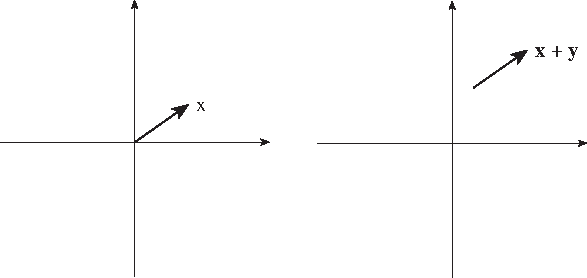
\includegraphics[width=2in]{Isometries}
}
\end{center}
\caption{Translations in ${\Bbb R}^2$}
\label{Isometries}
\end{figure}
 
 
 
 
 
\section{Symmetry}
 
 
 
 
An {\bfi isometry\/}\index{Isometry} or {\bfi rigid
motion\/}\index{Rigid motion} in ${\Bbb R}^n$  is a
distance-preserving function $f$ from ${\Bbb R}^n$ to ${\Bbb R}^n$.
This means that $f$ must satisfy 
\[
\| f({\bold x}) - f({\bold y}) \| =
\|{\bold x} - {\bold y} \|
\]
for all ${\bold x}, {\bold y} \in {\Bbb R}^n$. It is not difficult to
show that $f$ must be a one-to-one map. By Theorem~10.2, any element in
$O(n)$ is an isometry on ${\Bbb R}^n$; however, $O(n)$ does not
include all possible isometries on ${\Bbb R}^n$. Translation by a
vector ${\bold x}$, $T_{\bold y}({\bold x}) = {\bold x} + {\bold y}$
is also an isometry (Figure~\ref{Isometries}); however, $T$ cannot be
in $O(n)$ since it is not a linear map. 
 
 
 
We are mostly interested in isometries in ${\Bbb R}^2$. In fact, the
only isometries in ${\Bbb R}^2$ are rotations and reflections  about
the origin, translations, and combinations of the two. For example, a
{\bfi glide reflection\/}\index{Glide reflection} is a translation
followed by a reflection (Figure~\ref{Glide}).   In ${\Bbb R}^n$ all
isometries are given in the same manner. The proof is very easy to
generalize. 
 
 
\begin{figure}[htb]
\begin{center}
\centerline {
\includegraphics[width=2in]{Glide}
}
\end{center}
\caption{Glide reflections}
\label{Glide}
\end{figure}
 
 
\begin{lemma}
An isometry $f$ that fixes the origin in ${\Bbb R}^2$ is a linear
transformation.  In particular, $f$ is given by an element in $O(2)$. 
\end{lemma}
 
 
\begin{proof}
Let $f$ be an isometry in ${\Bbb R}^2$ fixing the origin. We will
first show that $f$ preserves inner products. Since $f(0) = 0$, $\|
f({\bold x})\| = \| {\bold x} \|$; therefore,
\begin{eqnarray*}
\| {\bold x} \|^2 - 2 \langle f({\bold x}), f({\bold y}) \rangle + \|
{\bold y} \|^2 
& = &
\| f({\bold x}) \|^2 - 2 \langle f({\bold x}), f({\bold y}) \rangle +
\| f({\bold y}) \|^2 \\ 
& = &
\langle
f({\bold x}) -  f({\bold y}), f({\bold x}) -  f({\bold y})
\rangle \\
& = &
\| f({\bold x}) -  f({\bold y}) \|^2 \\
& = &
\| {\bold x} -  {\bold y} \|^2 \\
& = &
\langle
{\bold x} -  {\bold y}, {\bold x} -  {\bold y} \rangle \\
& = &
\| {\bold x} \|^2 - 2 \langle {\bold x}, {\bold y} \rangle + \| {\bold
y} \|^2. 
\end{eqnarray*}
Consequently,
\[
\langle f({\bold x}), f({\bold y}) \rangle
=
\langle {\bold x}, {\bold y} \rangle.
\]
Now let ${\bold e}_1$ and ${\bold e_2}$ be $(1, 0)^{\rm t}$ and $(0,
1)^{\rm t}$, respectively. If 
\[
{\bold x} = (x_1, x_2) = x_1 {\bold e}_1 + x_2 {\bold e}_2,
\]
then
\[
f({\bold x})
=
\langle
f({\bold x}), f({\bold e}_1)
\rangle
f({\bold e}_1)
+\langle
f({\bold x}), f({\bold e}_2)
\rangle
f({\bold e}_2)
=
x_1 f({\bold e}_1)+x_2 f({\bold e}_2).
\]
The linearity of $f$ easily follows.
\end{proof}
 
 
\vspace{1.5ex}
 
 
For any arbitrary isometry, $f$,  $T_{\bold x} f$ will fix the origin
for some vector ${\bold x}$ in ${\Bbb R}^2$; hence, $T_{\bold x}
f({\bold y}) = A {\bold y}$ for some matrix $A \in O(2)$.
Consequently, $f({\bold y}) = A {\bold y} + {\bold x}$.  Given the
isometries 
\begin{eqnarray*}
f({\bold y}) & = & A {\bold y} + {\bold x}_1 \\
g({\bold y}) & = & B {\bold y} + {\bold x}_2,
\end{eqnarray*}
their composition is
\[
f(g({\bold y})) =
f(B {\bold y} + {\bold x}_2) =
AB {\bold y} + A{\bold x}_2 + {\bold x}_1.
\]
This last computation allows us to identify the group of isometries on
${\Bbb R}^2$ with~$E(2)$. 
 
 
\begin{theorem}
The group of isometries on ${\Bbb R}^2$ is the Euclidean group,
$E(2)$. 
\end{theorem}
 
 
A {\bfi symmetry group\/}\index{Group!symmetry} in ${\Bbb R}^n$ is a
subgroup of the group of isometries on ${\Bbb R}^n$ that fixes a set
of points $X \subset {\Bbb R}^2$.  It is important to realize that the
symmetry group of $X$ depends {\em both\/} on ${\Bbb R}^n$ and on
$X$. For example, the symmetry group of the origin in ${\Bbb R}^1$ is
${\Bbb Z}_2$, but the symmetry group of the origin in ${\Bbb R}^2$ is
$O(2)$. 
 
 
\begin{theorem}
The only finite symmetry groups in ${\Bbb R}^2$ are ${\Bbb Z}_n$ and
$D_n$. 
\end{theorem}
 
 
\begin{proof}
Any finite symmetry group $G$ in ${\Bbb R}^2$ must be a finite
subgroup of $O(2)$; otherwise, $G$ would have an element in $E(2)$ of
the form $(A, {\bold x})$, where ${\bold x} \neq 0$.  Such an element
must have infinite order. 
 
 
By Example~6, elements in $O(2)$ are either rotations of the form
\[
R_{\theta}
=
\left(
\begin{array}{cc}
\cos \theta & - \sin \theta \\
\sin \theta & \cos \theta
\end{array}
\right)
\]
or reflections of the form
\[T_{\theta}
=
\left(
\begin{array}{cc}
\cos \theta & - \sin \theta \\
\sin \theta & \cos \theta
\end{array}
\right).
\]
Notice that $\det(R_{\theta})=1$,  $\det(T_{\theta})=-1$,
and $T_{\theta}^2=I$. We can divide the proof up into two cases.  In
the first case, all of the elements in $G$ have determinant one. In the
second case, there exists at least one element in $G$ with 
determinant~$-1$.  
 
 
{\em Case 1.}  
The determinant of every element in $G$ is one. In this case every
element in $G$ must be a rotation. Since $G$ is finite, there is a
smallest angle, say $\theta_0$, such that the corresponding element
$R_{\theta_0}$ is the smallest rotation in the positive direction.  We
claim that $R_{\theta_0}$ generates $G$.  If not, then for some
positive integer $n$ there is an angle $\theta_1$ between $n \theta_0$
and $(n+1) \theta_0$. If so, then $(n+1) \theta_0 - \theta_1$
corresponds to a rotation smaller than $\theta_0$, which contradicts
the minimality of $\theta_0$.   
 
 
 
{\em Case 2.}  
The group $G$ contains a reflection $T_{\theta}$.  The kernel of the
homomorphism $\phi : G \rightarrow \{-1, 1\}$ given by $A \mapsto
\det(A)$ consists of elements whose determinant is 1.  Therefore, $|G/
\ker \phi|=2$.  We know that the kernel is cyclic by the first case
and is a subgroup of $G$ of, say, order $n$. Hence, $|G| = 2n$. The
elements of $G$ are
\[
R_{\theta}, \ldots, R_{\theta}^{n-1},  TR_{\theta}, \ldots,
TR_{\theta}^{n-1}.
\]
These elements satisfy the relation
\[
TR_{\theta}T = R_{\theta}^{-1}.
\]
Consequently, $G$ must be isomorphic to $D_n$ in this case.
\end{proof}
 
 
 
 
\begin{figure}[thb]
\begin{center}
\centerline {

\includegraphics[width=2in]{Wallpaper}
}
\end{center}
\caption{A wallpaper pattern in ${\Bbb R}^2$}
\label{Wallpaper}
\end{figure}
 
 
 
\subsection*{The Wallpaper Groups}
 
 
 
Suppose that we wish to study wallpaper patterns in the plane or
crystals in three dimensions. Wallpaper patterns are simply repeating
patterns in the plane (Figure~\ref{Wallpaper}). The analogs of
wallpaper patterns in ${\Bbb R}^3$ are crystals, which we can think of
as repeating patterns of molecules in three dimensions
(Figure~\ref{Crystals}). The mathematical equivalent of a wallpaper or
crystal pattern is called a  lattice. 
 
 
 
\begin{figure}[hbt]
\begin{center}
\centerline {
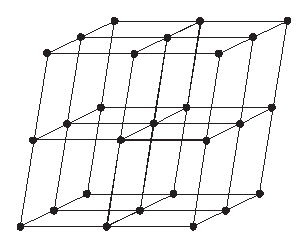
\includegraphics[width=2in]{Crystals}
}
\end{center}
\caption{A crystal structure in ${\Bbb R}^3$}
\label{Crystals}
\end{figure}
 
 

Let us examine wallpaper patterns in the plane a
little more closely. Suppose that ${\bold x}$ and ${\bold y}$ are
linearly independent vectors in ${\Bbb R}^2$; that is, one vector
cannot be a scalar multiple of the other. A {\bfi
lattice\/}\index{Lattice of points} of ${\bold x}$ and ${\bold y}$ is
the set of all linear combinations $m {\bold x} + n {\bold y}$, where
$m$ and $n$ are integers. The vectors ${\bold x}$ and ${\bold y}$ are
said to be a {\bfi basis\/}\index{Basis of a lattice} for the lattice.
 
 
\begin{figure}[htb]
\begin{center}
\centerline {
\includegraphics[width=2in]{LatticeExample}
}
\end{center}
\caption{A lattice in  ${\Bbb R}^2$}
\label{lattice}
\end{figure}
 
 
Notice that a lattice can have several bases. For example, the vectors
$(1,1)^{\rm t}$ and $(2,0)^{\rm t}$ have the  same lattice as the
vectors $(-1, 1)^{\rm t}$ and $(-1, -1)^{\rm t}$
(Figure~\ref{lattice}). However, any lattice is completely determined
by a basis. Given two bases for the same lattice, say $\{ {\bold x}_1,
{\bold x}_2 \}$ and $\{ {\bold y}_1, {\bold y}_2 \}$, we can write 
\begin{eqnarray*}
{\bold y}_1 & = & \alpha_1  {\bold x}_1 + \alpha_2 {\bold x}_2 \\
{\bold y}_2 & = & \beta_1  {\bold x}_1 + \beta_2 {\bold x}_2,
\end{eqnarray*}
where $\alpha_1$, $\alpha_2$, $\beta_1$, and $\beta_2$ are integers.
The matrix corresponding to this transformation is 
\[
U
=
\left(
\begin{array}{cc}
\alpha_1 & \alpha_2 \\
\beta_1 & \beta_2
\end {array}
\right).
\]
If we wish to give ${\bold x}_1$ and ${\bold x}_2$ in terms of ${\bold
y}_1$ and ${\bold y}_2$, we need only calculate $U^{-1}$; that is, 
\[
U^{-1}
\left(
\begin{array}{c}
{\bold y}_1 \\
{\bold y}_2
\end{array}
\right)
=
\left(
\begin{array}{c}
{\bold x}_1 \\
{\bold x}_2
\end{array}
\right).
\]
Since $U$ has integer entries, $U^{-1}$ must also have integer
entries; hence the determinants of both $U$ and $U^{-1}$ must be
integers. Because $U U^{-1} = I$,  
\[
\det(U U^{-1}) =\det(U) \det( U^{-1}) = 1;
\]
consequently, $\det(U) = \pm 1$. A matrix with determinant $\pm 1$ and
integer entries is called {\bfi unimodular}\index{Matrix!unimodular}.
For example, the matrix 
\[
\left(
\begin{array}{cc}
3 & 1 \\
5 & 2
\end{array}
\right)
\]
is unimodular. It should be clear that there is a minimum length for
vectors in a lattice.  
 
 
We can classify lattices by studying their symmetry groups. The
symmetry group of a lattice is the subgroup of $E(2)$ that maps the
lattice to itself. We consider two lattices in ${\Bbb R}^2$ to be
equivalent if they have the same symmetry group.  Similarly,
classification of crystals in ${\Bbb R}^3$ is accomplished by
associating a symmetry group, called a {\bfi space group}, with each
type of crystal\index{Group!space}. Two lattices are considered
different if their space groups are not the same.  The natural
question that now arises is how many space groups exist. 
 
 
A space group is composed of two parts: a {\bfi translation
subgroup\/}\index{Subgroup!translation} and a {\bfi point
group}\index{Group!point}.  The translation subgroup is an infinite
abelian subgroup of the space group made up of the translational
symmetries of the crystal; the point group is a finite group 
consisting  of rotations and reflections of the crystal about a point.
More specifically, a space group is a subgroup of $G \subset E(2)$
whose translations are a set of the form $\{ (I, t) : t \in L \}$,
where $L$ is a lattice. Space groups are, of course, infinite. Using
geometric arguments, we can prove the following theorem (see [5] or [6]).
 
 
 
 
\begin{theorem}
Every translation group in ${\Bbb R}^2$ is isomorphic to ${\Bbb Z}
\times {\Bbb Z}$.
\end{theorem}
 
 
\begin{figure}[bht]
\begin{center}
\centerline {
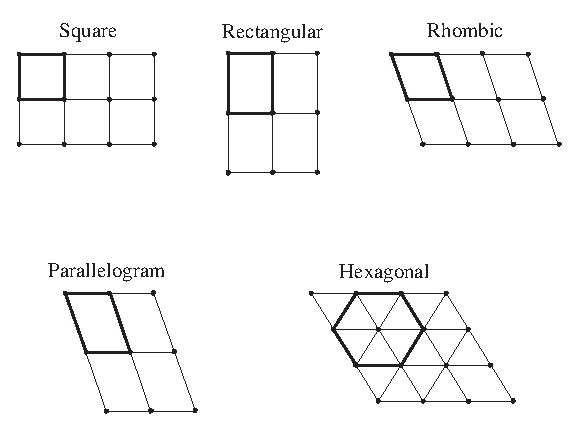
\includegraphics[width=2in]{TypeLattice}
}
\end{center}
\caption{Types of lattices in  ${\Bbb R}^2$}
\label{Types}
\end{figure}
 
 
The point group of $G$ is $G_0 = \{A : (A,b) \in G \mbox{ for some
$b$}  \}$. In particular, $G_0$ must be a subgroup of $O(2)$. Suppose
that ${\bold x}$ is a vector in a lattice $L$ with space group $G$,
translation group $H$, and point group $G_0$. For any element $(A,
{\bold y})$ in $G$,   
\begin{eqnarray*}
(A, {\bold y}) (I, {\bold x}) (A, {\bold y})^{-1}
& = &
(A,A {\bold x} + {\bold y}) (A^{-1},-A^{-1} {\bold y}) \\
& = &
(A A^{-1},-A A^{-1} {\bold y} + A {\bold x} + {\bold y}) \\
& = &
(I, A {\bold x});
\end{eqnarray*}
hence, $(I, A {\bold x})$ is in the translation group of $G$. More
specifically, $A {\bold x}$ must be in the lattice $L$. It is
important to note that $G_0$ is not usually a subgroup of the space
group $G$; however, if $T$ is the translation subgroup of $G$, then
$G/T \cong G_0$. The proof of the following theorem can be found in
[2], [5], or~[6].
 
 
 
\begin{theorem}
The point group in the wallpaper groups is isomorphic to ${\Bbb Z}_n$
or $D_n$, where $n = 1, 2, 3, 4, 6$. 
\end{theorem}
 
 
To answer the question of how the point groups and the translation
groups can be combined, we must look at the different types of
lattices. Lattices can be classified by the structure of a single
lattice cell. The possible cell shapes are parallelogram, rectangular,
square, rhombic, and hexagonal (Figure~\ref{Types}). The wallpaper
groups can now be classified according to the types of reflections
that occur in each group: these are ordinarily reflections, glide
reflections, both, or none.
 
 
 
\begin{table}[htb]
\caption{The 17 wallpaper groups}{\small
\begin{center}
\begin{tabular}{|l|l|l|l|}
\hline
Notation and &             &              & Reflections  \\
Space Groups & Point Group & Lattice Type & or Glide Reflections? \\
\hline
p1 & ${\Bbb Z}_1$ & parallelogram & none \\
p2 & ${\Bbb Z}_2$ & parallelogram & none \\
p3 & ${\Bbb Z}_3$ & hexagonal & none \\
p4 & ${\Bbb Z}_4$ & square & none \\
p6 & ${\Bbb Z}_6$ & hexagonal & none \\
pm & $D_1$ & rectangular & reflections \\
pg & $D_1$ & rectangular & glide reflections\\
cm & $D_1$ & rhombic & both \\
pmm & $D_2$ & rectangular & reflections \\
pmg & $D_2$ & rectangular & glide reflections \\
pgg & $D_2$ & rectangular & both \\
c2mm & $D_2$ & rhombic & both \\
p3m1, p31m & $D_3$ & hexagonal & both \\
p4m, p4g & $D_4$ & square & both \\
p6m & $D_6$ & hexagonal & both \\
\hline
\end{tabular}
\end{center}
}
\end{table}
 
 
\begin{theorem}
There are exactly 17 wallpaper groups.
\end{theorem}
 
 
\begin{figure}[htb]
\begin{center}
\centerline {
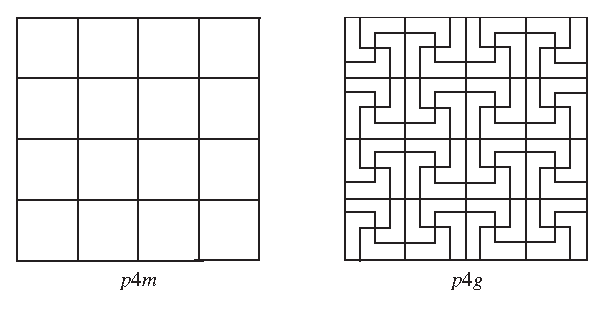
\includegraphics[width=2in]{p4m}
}
\end{center}
\caption{The wallpaper groups p4m and  p4g}
\label{p4m}
\end{figure}
 
 
 
The 17 wallpaper groups are listed in Table~10.1. The groups p3m1 and
p31m can be distinguished by whether or not all of their threefold
centers lie on the reflection axes: those of p3m1 must, whereas those
of p31m may not. Similarly, the fourfold centers of p4m must lie on
the reflection axes whereas those of p4g need not (Figure~\ref{p4m}).
The complete proof of this theorem can be found in several of the
references at the end of this chapter, including [5], [6], [10],
and~[11]. 
 
 
 
\histhead
 
 
\noindent{\small \histf
Symmetry groups have intrigued mathematicians for a long time.
Leonardo da Vinci was probably the first person to know all of the
point groups.  At the International Congress of Mathematicians in
1900, David Hilbert\index{Hilbert, David} gave a now-famous address
outlining 23 problems to guide mathematics in the twentieth
century.  Hilbert's eighteenth problem asked whether or not
crystallographic groups in $n$ dimensions were always finite.  In
1910, L.~Bieberbach\index{Bieberbach, L.} proved that crystallographic
groups are finite in every dimension.  Finding out how many of these
groups there are in each dimension is another matter. In ${\Bbb R}^3$
there are 230 different space groups; in ${\Bbb R}^4$ there are 4783.
No one has been able to compute the number of space groups for ${\Bbb
R}^5$ and beyond. It is interesting to note that the crystallographic
groups were found mathematically for ${\Bbb R}^3$ before the 230
different types of crystals were actually discovered in nature.
\histbox
}
 
 
 
\markright{EXERCISES}
\section*{Exercises}
\exrule
 
 
{\small
\begin{enumerate}
 
 
 
\bf\item\rm
Prove the identity
\[
\langle {\bold x}, {\bold y} \rangle = \frac{1}{2}
\left[
\|{\bold x} + {\bold y}\|^2 - \|{\bold x}\|^2 - \| {\bold y}\|^2
\right].
\]
 
 
\bf\item\rm
Show that $O(n)$ is a group.
 
 
\bf\item\rm
Prove that the following matrices are orthogonal. Are any of
these matrices in $SO(n)$?
 
\vspace{3pt}        %two column exercise list
 
\hspace{-7pt}
\begin{minipage}[t]{4.6in}
\noindent
\begin{minipage}[t]{2.25in}
\begin{itemize}
 
 \item[{\bf (a)}]
\raisebox{-5.5pt}{\parbox{1.85in}{
\[
\left(
\begin{array}{cc}
1/\sqrt{2} & -1/\sqrt{2} \\
1/\sqrt{2} & 1/\sqrt{2}
\end{array}
\right)
\]
}}

 
 \item[{\bf (c)}]
\raisebox{-11.5pt}{\parbox{1.85in}{
\[
\left(
\begin{array}{ccc}
4/ \sqrt{5} & 0 & 3 / \sqrt{5} \\
-3 / \sqrt{5} & 0 & 4 / \sqrt{5} \\
0 & -1 & 0
\end{array}
\right)
\] 
}}

\end{itemize}
\end{minipage} \hfill
\begin{minipage}[t]{2.25in}
\begin{itemize}
 
 \item[{\bf (b)}]
\raisebox{-5.5pt}{\parbox{1.85in}{
\[
\left(
\begin{array}{cc}
1 / \sqrt{5} & 2 / \sqrt{5} \\
- 2 /\sqrt{5} & 1/ \sqrt{5}
\end{array}
\right)
\]
}} 
 
 
 \item[{\bf (d)}]
\raisebox{-11.5pt}{\parbox{1.85in}{
\[
\left(
\begin{array}{ccc}
1/3 & 2/3 & - 2/3 \\
- 2/3 & 2/3 & 1/3 \\
-2/3 & 1/3 & 2/3
\end{array}
\right)
\]
}}
 
 
\end{itemize}
\end{minipage}
\end{minipage}
 
\vspace{2pt}        %end two column exercise list
 
 
 
\bf\item\rm %%%%%%%%%%%%%%%%%%%%%%
Determine the symmetry group of each of the figures in
Figure~\ref{Determine}. 
\begin{figure}[htb]
\begin{center}
\centerline {
\includegraphics[width=2in]{SymmetryGrp}
}
\end{center}
\caption{}
\label{Determine}
\end{figure}
 
 
\bf\item\rm
Let ${\bold x}$, ${\bold y}$, and ${\bold w}$ be vectors in ${\Bbb
R}^n$ and $\alpha \in {\Bbb R}$.  Prove each of the following
properties of inner products.
\begin{enumerate}
 
 \bf\item\rm
$\langle {\bold x}, {\bold y} \rangle = \langle {\bold y}, {\bold x}
\rangle$. 
 
 \bf\item\rm
$\langle {\bold x}, {\bold y} + {\bold w} \rangle = \langle
{\bold x}, {\bold y} \rangle + \langle {\bold x}, {\bold w}
\rangle$.
 
 \bf\item\rm
$\langle \alpha {\bold x}, {\bold y} \rangle = \langle
{\bold x}, \alpha {\bold y} \rangle = \alpha \langle  {\bold
x}, {\bold y} \rangle$.
 
 \bf\item\rm
$\langle {\bold x}, {\bold x} \rangle \geq 0$ with equality exactly
when ${\bold x} = 0$. 
 
 \bf\item\rm
If $\langle {\bold x}, {\bold y} \rangle = 0$  for all ${\bold x}$ in
${\Bbb R}^n$, then ${\bold y} = 0$. 
 
\end{enumerate}
 
 
\bf\item\rm
Verify that
\[
E(n)
=
\{(A, {\bold x}) : A \in O(n) \mbox{ and } {\bold x} \in
{\Bbb R}^n \}
\]
is a group.
 
 
\bf\item\rm
Prove that $\{ (2,1), (1,1) \}$  and $\{ ( 12, 5), ( 7, 3) \}$ are bases
for the same lattice. 
 
 
\bf\item\rm
Let $G$ be a subgroup of $E(2)$ and suppose that $T$ is the
translation subgroup of $G$.  Prove that the point group of $G$ is
isomorphic to $G/T$. 
 
 
\bf\item\rm
Let $A \in SL_2({\Bbb R})$ and suppose that the vectors ${\bold x}$
and ${\bold y}$ form two sides of a parallelogram in ${\Bbb R}^2$.
Prove that the area of this parallelogram is the same as the area of
the parallelogram with sides $A{\bold x}$ and $A{\bold y}$. 
 
 
\bf\item\rm
Prove that $SO(n)$ is a normal subgroup of $O(n)$.
 
 
\bf\item\rm
Show that any isometry $f$ in ${\Bbb R}^n$ is a one-to-one map.
 
 
\bf\item\rm
Show that an element in $E(2)$ of the form $(A, {\bold x})$,
where ${\bold x} \neq 0$, has infinite order.
 
 
\bf\item\rm
Prove or disprove: There exists an infinite abelian subgroup of 
$O(n)$.
 
 
\bf\item\rm
Let ${\bold x} = (x_1, x_2)$ be a point on the unit circle in ${\Bbb
R}^2$; that is, $x_1^2 + x_2^2 = 1$. If $A \in O(2)$, show that $A
{\bold x}$ is also a point on the unit circle. 
 
 
 
\bf\item\rm
Let $G$ be a group with a subgroup $H$ (not necessarily normal) and a
normal subgroup $N$. Then $G$ is a {\bfi semidirect
product\/}\index{Semidirect product} of $N$ by $H$ if  
\begin{itemize}
 
 \item
$H \cap N = \{ id \}$;
 
 \item
$HN=G$.
 
\end{itemize}
Show that each of the following is true.
\begin{enumerate}
 
 \bf\item\rm
$S_3$ is the semidirect product of $A_3$ by $H = \{(1), (12) \}$.
 
 \bf\item\rm
The quaternion group, $Q_8$, cannot be written as a semidirect product. 
 
 \bf\item\rm
$E(2)$ is the semidirect product of $O(2)$ by $H$, where $H$ consists
of all translations in ${\Bbb R}^2$. 
 
\end{enumerate}
 
 
 
\bf\item\rm
Determine which of the 17 wallpaper groups preserves the symmetry of
the pattern in Figure~\ref{Wallpaper}.  
 
\begin{figure}[htb]
\begin{center}
\centerline {
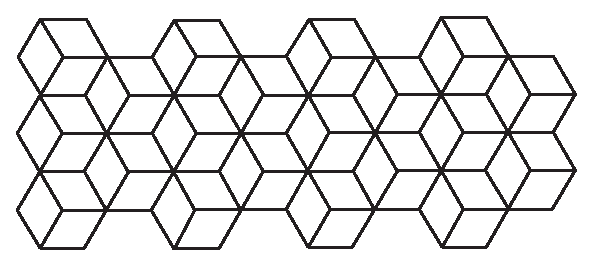
\includegraphics[width=2in]{p6m}
}
\end{center}
\caption{}
\label{For17}
\end{figure}
 
\bf\item\rm
Determine which of the 17 wallpaper groups preserves the symmetry of
the pattern in Figure~\ref{For17}.  
 
 
 
\bf\item\rm
Find the rotation group of a dodecahedron.
 
  
 
\bf\item\rm
For each of the 17 wallpaper groups, draw a wallpaper pattern having
that group as a symmetry group.  
 
\end{enumerate}
}
 
 
 
\subsection*{References and Suggested Readings}
 
 
 
{\small
\begin{itemize}
 
\item[{\bf [1]}]
Coxeter, H. M. and Moser, W. O. J. {\it Generators and
Relations for Discrete Groups}, 3rd ed. Springer-Verlag, New
York, 1972.
 
\item[{\bf [2]}]
Grove, L. C. and Benson, C. T. {\it Finite Reflection
Groups}. 2nd ed. Springer-Verlag, New York, 1985.
 
\item[{\bf [3]}]
Hiller, H. ``Crystallography and Cohomology of Groups,''
{\it American Mathematical Monthly} {\bf 93} (1986), 765--79.
 
\item[{\bf [4]}]
Lockwood, E. H. and Macmillan, R. H. {\it Geometric
Symmetry}. Cambridge University Press, Cambridge, 1978.
 
\item[{\bf [5]}]
Mackiw, G. {\it Applications of Abstract Algebra}. Wiley,
New York, 1985.
 
 
\item[{\bf [6]}]
Martin,  G.  {\it Transformation  Groups:  An Introduction to
Symmetry}.  Springer-Verlag, New York, 1982.
 
  
\item[{\bf [7]}]
Milnor, J. ``Hilbert's Problem 18: On Crystallographic
Groups, Fundamental Domains, and Sphere Packing,'' {\it
Proceedings of Symposia in Pure Mathematics} {\bf 18},
American Mathematical Society, 1976.
 
\item[{\bf [8]}]
Phillips, F. C. {\it An Introduction to Crystallography}.
4th ed. Wiley, New York, 1971.
 
\item[{\bf [9]}]
Rose, B. I. and Stafford, R. D. ``An Elementary Course in
Mathematical Symmetry,'' {\it American Mathematical Monthly} {\bf
88} (1980), 54--64.
 
 
\item[{\bf [10]}]
Schattschneider, D. ``The Plane Symmetry Groups: Their
Recognition and Their Notation,'' {\it American Mathematical 
Monthly} {\bf 85} (1978), 439--50.
 
 
\item[{\bf [11]}]
Schwarzenberger, R. L. ``The 17 Plane Symmetry Groups,'' {\it
Mathematical  Gazette} {\bf 58} (1974), 123--31. 
 
 
\item[{\bf [12]}]
Weyl, H. {\it Symmetry}. Princeton University Press, Princeton, NJ,
1952. 
 
 
\end{itemize}
}
 
 
 
 
   %Groups of Symmetries
There are no exercises for this section.   %Abelian and Solvable Groups
%%%%(c)
%%%%(c)  This file is a portion of the source for the textbook
%%%%(c)
%%%%(c)    Abstract Algebra: Theory and Applications
%%%%(c)    by Thomas W. Judson
%%%%(c)
%%%%(c)    Sage Material
%%%%(c)    Copyright 2011 by Robert A. Beezer
%%%%(c)
%%%%(c)  See the file COPYING.txt for copying conditions
%%%%(c)
%%%%(c)
Groups can be realized in many ways, such as as sets of permutations, as sets of matrices, or as sets of abstract symbols related by certain rules (``presentations'') and in myriad other ways.  We have concentrated on permutation groups because of their concrete feel with elements written as functions and because of their thorough implementation in Sage.  Group actions are of great interest when the set they act on is the group itself, and that will be the main application of this chapter in the next chapter.  However, any time we have a group action on a set, we can view that group as a permutation group on the elements of the set.  So permutation groups are an area of group theory of independent interest with its own definitions and theorems.\par
%
We will describe Sage's commands applicable when a group action arises naturally via conjugation, and then move into the more general situation in a more general application.\par
%
\sagesubsection{Conjugation as a Group Action}
%
We might think we need to be careful how Sage defines conjugation ($gxg^{-1}$ versus $g^{-1}xg$) and the difference between Sage and the text on the order of products.  However, if you look at the definition of the center and centralizer subgroups you can see that any difference in ordering is irrelevant.  Here are the group action commands for the particular action that is conjugation of the elements of the group.\par
%
Sage has a permutation group method \verb?.center()? which returns the subgroup of fixed points.  The permutation group method, \verb?.centralizer(g)?, returns a subgroup that is the stabilizer of the group element \verb?g?.  Finally, the orbits are given by conjugacy classes, but Sage will not flood you with the full conjugacy classes and instead gives back a list of one element per conjugacy class, the representatives, via the permutation group method \verb?.conjugacy_classes_representatives()?.  You can manually reconstruct a conjugacy class from a representative, as we do in the example below.\par
%
Here is an example of the above commands in action.  Notice that an abelian group would be a bad choice for this example.
%
\begin{sageexample}
sage: D = DihedralGroup(8)
sage: C = D.center(); C
Subgroup of (Dihedral group of order 16 as a permutation group) 
generated by [(1,5)(2,6)(3,7)(4,8)]
sage: C.list()
[(), (1,5)(2,6)(3,7)(4,8)]
sage: a = D("(1,2)(3,8)(4,7)(5,6)")
sage: C1 = D.centralizer(a); C1.list()
[(), (1,2)(3,8)(4,7)(5,6), (1,5)(2,6)(3,7)(4,8), (1,6)(2,5)(3,4)(7,8)]
sage: b = D("(1,2,3,4,5,6,7,8)")
sage: C2 = D.centralizer(b); C2.order()
8
sage: CCR = D.conjugacy_classes_representatives(); CCR
[(), (2,8)(3,7)(4,6), (1,2)(3,8)(4,7)(5,6), (1,2,3,4,5,6,7,8),
 (1,3,5,7)(2,4,6,8), (1,4,7,2,5,8,3,6), (1,5)(2,6)(3,7)(4,8)]
sage: r = CCR[2]; r
(1,2)(3,8)(4,7)(5,6)
sage: conj = []
sage: x = [conj.append(g^-1*r*g) for g in D if not g^-1*r*g in conj]
sage: conj
[(1,2)(3,8)(4,7)(5,6), (1,8)(2,7)(3,6)(4,5), (1,4)(2,3)(5,8)(6,7),
 (1,6)(2,5)(3,4)(7,8)]
\end{sageexample}
%
Notice that in the one conjugacy class constructed all the elements have the same cycle structure, which is no accident.  Notice too that \verb?rep? and \verb?a? are the same element, and the product of the order of the centralizer ($4$) and the size of the conjugacy class ($4$) equals the order of the group ($16$), which is a variant of Theorem~\ref{orbit_theorem}.\par
%
Verify that the following is a demonstration of the class equation in the special case when the action is conjugation, but would be valid for any group, rather than just \verb?D?.
%
\begin{sageexample}
sage: sizes = [D.order()/D.centralizer(g).order()
...                for g in D.conjugacy_classes_representatives()]
sage: sizes
[1, 4, 4, 2, 2, 2, 1]
sage: D.order() == sum(sizes)
True
\end{sageexample}
%
\sagesubsection{Graph Automorphisms}
%
As mentioned, group actions can be even more interesting when the set they act on is different from the group itself.  One class of examples is the group of symmetries of a geometric solid, where the objects in the set are the vertices of the object, or perhaps some other aspect such as edges, faces or diagonals.  In this case, the group is all those permutations that move the solid but leave it filling the same space before the motion (``rigid motions'').\par
%
In this section we will examine something very similar.  A {\bf graph} is a mathematical object, consisting of vertices and edges, but the only structure is whether or not any given pair of vertices are joined by an edge or not.  The group consists of permutations of vertices that preserve the structure, that is, permutaions of vertices that take edges to edges and non-edges to non-edges.  It is very similar to a symmetry group, but there is no notion of any geometric relationships being preserved.\par
%
Here is an example.  You will need to run the first compute cell to define the graph and get a nice graphic representation.
%
\begin{sageexample}
sage: Q = graphs.CubeGraph(3)
sage: Q.plot(layout='spring')      # not tested
\end{sageexample}
%
\begin{sageexample}
sage: A = Q.automorphism_group()
sage: A.order()
48
\end{sageexample}
%
Your plot should look like the vertices and edges of a cube, but may not quite look regular, which is fine, since the geometry is not relevant.  Vertices are labeled with strings of three binary digits, $0$ or $1$, and any two vertices are connected by an edge if their strings differ in exactly one location.  We might expect the group of symmetries to have order 24, rather than order 48, given its resemblance to a cube (in appearance and in name).  However, when not restricted to rigid motions, we have new permutations that preserve edges.  One in particular is to interchange two ``opposite faces.''  Locate two $4$-cycles opposite of each other, listed in the same order:  $000, 010, 110, 100$ and $001, 011, 111, 101$.  Notice that each cycle looks very similar, but all the vertices of the first end in a zero and the second cycle has vertices ending in a one.\par
%
We can create this permutation explicitly from a text version in cycle notation.
%
\begin{sageexample}
sage: a = A("('000','001')('010','011')('110','111')('100','101')")
sage: a in A
True
\end{sageexample}
%
We can use this group to illustrate the relevant Sage commands for group actions.
%
\begin{sageexample}
sage: A.orbits()
[['000', '001', '010', '100', '011', '101', '110', '111']]
\end{sageexample}
%
So this action has only one (big) orbit.  This implies that every vertex is ``like'' any other.  When a permutation group behaves this way, we say it is ``transitive''.
%
\begin{sageexample}
sage: A.is_transitive()
True
\end{sageexample}
%
If every vertex is ``the same'' we can compute the stabilizer of any vertex, since they will all be isomorphic.  Because vertex $000$ is the simplest in some sense, we compute its stabilizer.
%
\begin{sageexample}
sage: S = A.stabilizer('000')
sage: S.list()
[(),
 ('010','100')('011','101'),
 ('001','010')('101','110'),
 ('001','010','100')('011','110','101'),
 ('001','100','010')('011','101','110'),
 ('001','100')('011','110')]
\end{sageexample}
%
That \verb?S? has $6$ elements is no surprise, since the group has order $48$ and the size of the lone orbit is $8$.  But we can go one step further.  The three vertices connected directly to $000$ are $100$, $010$, $001$, which are numbered $4, 2, 1$ in the permutation group.  Any automorphism of the graph that fixes $000 = 8$ must then permute the three adjacent vertices.  There are $3!=6$ possible ways to do this, and you can check that each appears in one of the six elements of the stabilizer.  So we can understand a transitive group by considering the smaller stabilizer, and in this case we can see that each element of the stabilizer is determined by how it permutes the neighbors of the stabilized vertex.
%
Transitive groups are both unusual and important.  To contrast, here is a graph automorphism group that is far from transitive (without being trivial).  A path is a graph that has all of its vertices in a line.  Run the first compute cell to see a path on 11 vertices.
%
%
\begin{sageexample}
sage: P = graphs.PathGraph(11)
sage: P.plot()       # not tested
\end{sageexample}
%
\begin{sageexample}
sage: A = P.automorphism_group()
sage: A.list()
[(), (0,10)(1,9)(2,8)(3,7)(4,6)]
\end{sageexample}
%
The automorphism group is the trivial identity automorphism (always) and an order 2 permutation that ``flips'' the path end-to-end.  The group is far from transitive and there are many orbits.
%
\begin{sageexample}
sage: A.is_transitive()
False
sage: A.orbits()
[[0, 10], [1, 9], [2, 8], [3, 7], [4, 6], [5]]
\end{sageexample}
%
Most of the stabilizers are trivial, with one exception.  As subgroups of a group of order 2, there really are not too many options.
%
\begin{sageexample}
sage: A.stabilizer(2).list()
[()]
sage: A.stabilizer(5).list()
[(), (0,10)(1,9)(2,8)(3,7)(4,6)]
\end{sageexample}
%
How would this final example have been different if we had used a path on 10 vertices?
%  %Group Actions
%%%%(c)
%%%%(c)  This file is a portion of the source for the textbook
%%%%(c)
%%%%(c)    Abstract Algebra: Theory and Applications
%%%%(c)    by Thomas W. Judson
%%%%(c)
%%%%(c)    Sage Material
%%%%(c)    Copyright 2011 by Robert A. Beezer
%%%%(c)
%%%%(c)  See the file COPYING.txt for copying conditions
%%%%(c)
%%%%(c)
\sagesubsection{Sylow Subgroups}
%
The Sage permutation group method \verb?.sylow_subgroup(p)? will return a single Sylow $p$-subgroup.  If the prime is not a proper divisor of the group order it returns a subgroup of order $p^0$, in other words, a trivial subgroup.  So be careful about the primes you choose.  Sometimes, you may only want \emph{one} such Sylow subgroup, since any two Sylow $p$-subgroups are conjugate, and hence isomorphic (Theorem~\ref{sylow:Sylow_two_theorem}).  This also means we can create other Sylow $p$-subgroups by conjugating the one we have.  The permutation group method \verb?.conjugate(g)? will conjugate the group by \verb?g?.\par
%
With repeated conjugations of a single Sylow $p$-subgroup, we will likely create duplicate subgroups.  So we need to use a slightly complicated construction to form a list of just the unique subgroups in the list of conjugates.  The list comprehension will modify the list of unique subgroups, but also create some output we do not care about, so we assign the unwanted output to the variable \verb?junk?.\par
%
Lets investigate the Sylow subgroups of the dihedral group $D_{18}$.  As a group of order $36=2^2\cdot 3^2$, we know by the First Sylow Theorem that there is a Sylow $2$-subgroup of order $4$ and a Sylow $3$-subgroup of order $9$.  First for $p=2$, we obtain one Sylow $2$-subgroup, form all the conjugates, and form a list of non-duplicate subgroups.  (These commands take a while to execute, so be patient.)
%
\begin{sageexample}
sage: G = DihedralGroup(18)
sage: S2 = G.sylow_subgroup(2); S2
Subgroup of (Dihedral group of order 36 as a permutation group) 
generated by 
[(2,18)(3,17)(4,16)(5,15)(6,14)(7,13)(8,12)(9,11), 
(1,10)(2,11)(3,12)(4,13)(5,14)(6,15)(7,16)(8,17)(9,18)]
sage: allS2 = [S2.conjugate(g) for g in G]
sage: uniqS2 = []
sage: junk = [uniqS2.append(H) for H in allS2 if not H in uniqS2]
sage: uniqS2
[Permutation Group with generators 
[(2,18)(3,17)(4,16)(5,15)(6,14)(7,13)(8,12)(9,11), 
(1,10)(2,11)(3,12)(4,13)(5,14)(6,15)(7,16)(8,17)(9,18)], 
Permutation Group with generators 
[(1,3)(4,18)(5,17)(6,16)(7,15)(8,14)(9,13)(10,12), 
(1,10)(2,11)(3,12)(4,13)(5,14)(6,15)(7,16)(8,17)(9,18)], 
Permutation Group with generators 
[(1,5)(2,4)(6,18)(7,17)(8,16)(9,15)(10,14)(11,13), 
(1,10)(2,11)(3,12)(4,13)(5,14)(6,15)(7,16)(8,17)(9,18)], 
Permutation Group with generators 
[(1,7)(2,6)(3,5)(8,18)(9,17)(10,16)(11,15)(12,14), 
(1,10)(2,11)(3,12)(4,13)(5,14)(6,15)(7,16)(8,17)(9,18)], 
Permutation Group with generators 
[(1,9)(2,8)(3,7)(4,6)(10,18)(11,17)(12,16)(13,15), 
(1,10)(2,11)(3,12)(4,13)(5,14)(6,15)(7,16)(8,17)(9,18)], 
Permutation Group with generators 
[(1,10)(2,11)(3,12)(4,13)(5,14)(6,15)(7,16)(8,17)(9,18), 
(1,11)(2,10)(3,9)(4,8)(5,7)(12,18)(13,17)(14,16)], 
Permutation Group with generators 
[(1,10)(2,11)(3,12)(4,13)(5,14)(6,15)(7,16)(8,17)(9,18), 
(1,13)(2,12)(3,11)(4,10)(5,9)(6,8)(14,18)(15,17)], 
Permutation Group with generators 
[(1,10)(2,11)(3,12)(4,13)(5,14)(6,15)(7,16)(8,17)(9,18), 
(1,15)(2,14)(3,13)(4,12)(5,11)(6,10)(7,9)(16,18)], 
Permutation Group with generators 
[(1,10)(2,11)(3,12)(4,13)(5,14)(6,15)(7,16)(8,17)(9,18), 
(1,17)(2,16)(3,15)(4,14)(5,13)(6,12)(7,11)(8,10)]]
sage: len(uniqS2)
9
\end{sageexample}
%
The Third Sylow Theorem tells us that for $p=2$ we would expect $1, 3\text{ or }9$ Sylow $2$-subgroups, so our computational result of 9 subgroups is consistent with what the theory predicts.  Can you visualize each of these subgroups as symmetries of an $18$-gon?  Notice that we also have many subgroups of order $2$ inside of these subgroups of order $4$.
%
\begin{sageexample}
sage: G = DihedralGroup(18)
sage: S3 = G.sylow_subgroup(3); S3
Subgroup of (Dihedral group of order 36 as a permutation group) 
generated by 
[(1,7,13)(2,8,14)(3,9,15)(4,10,16)(5,11,17)(6,12,18), 
(1,15,11,7,3,17,13,9,5)(2,16,12,8,4,18,14,10,6)]
sage: allS3 = [S3.conjugate(g) for g in G]
sage: uniqS3 = []
sage: junk = [uniqS3.append(H) for H in allS3 if not H in uniqS3]
sage: uniqS3
[Permutation Group with generators 
[(1,7,13)(2,8,14)(3,9,15)(4,10,16)(5,11,17)(6,12,18), 
(1,15,11,7,3,17,13,9,5)(2,16,12,8,4,18,14,10,6)]]
sage: len(uniqS3)
1
\end{sageexample}
%
What does the Third Sylow Theorem predict?  Just $1$ or $4$ Sylow $3$-subgroups.  Having found just one subgroup computationally, we know that all of the conjugates of the lone Sylow $3$-subgroup are equal.  In other words, the Sylow $3$-subgroup is normal in $D_{18}$.  Let's check.
%
\begin{sageexample}
sage: S3.is_normal(G)
True
\end{sageexample}
%
At least one of the subgroups of order $3$ contained in this Sylow $3$-subgroup should be obvious by looking at the orders of the generators, and then you may even notice that the generators given could be reduced, and one is a power of the other.
%
\begin{sageexample}
sage: S3.is_cyclic()
True
\end{sageexample}
%
Remember that there are many other subgroups, of other orders.  For example, can you construct a subgroup of order $6=2\cdot 3$ in $D_{18}$?\par
%
\sagesubsection{Normalizers}
%
A new command that is relevant to this section is the construction of a normalizer.  The Sage command \verb?G.normalizer(H)? will return the subgroup of \verb?G? containing elements that normalize the subgroup \verb?H?.  We illustrate its use with the Sylow subgroups from above.
%
\begin{sageexample}
sage: G = DihedralGroup(18)
sage: S2 = G.sylow_subgroup(2)
sage: S3 = G.sylow_subgroup(3)
sage: N2 = G.normalizer(S2); N2
Subgroup of (Dihedral group of order 36 as a permutation group) 
generated by 
[(2,18)(3,17)(4,16)(5,15)(6,14)(7,13)(8,12)(9,11), 
(1,10)(2,11)(3,12)(4,13)(5,14)(6,15)(7,16)(8,17)(9,18)]
sage: N2 == S2
True
sage: N3 = G.normalizer(S3); N3
Subgroup of (Dihedral group of order 36 as a permutation group) 
generated by 
[(2,18)(3,17)(4,16)(5,15)(6,14)(7,13)(8,12)(9,11), 
(1,2)(3,18)(4,17)(5,16)(6,15)(7,14)(8,13)(9,12)(10,11), 
(1,7,13)(2,8,14)(3,9,15)(4,10,16)(5,11,17)(6,12,18), 
(1,15,11,7,3,17,13,9,5)(2,16,12,8,4,18,14,10,6)]
sage: N3 == G
True
\end{sageexample}
%
The normalizer of a subgroup always contains the whole subgroup, so the normalizer of \verb?S2? is as small as possible.  We already knew \verb?S3? is normal in \verb?G?, so it is no surprise that its normalizer is as big as possible --- every element of \verb?G? normalizes \verb?S3?.  Let's compute a normalizer in $D_{18}$ that is more ``interesting.''
%
\begin{sageexample}
sage: G = DihedralGroup(18)
sage: a = G("(1,7,13)(2,8,14)(3,9,15)(4,10,16)(5,11,17)(6,12,18)")
sage: b = G("(1,5)(2,4)(6,18)(7,17)(8,16)(9,15)(10,14)(11,13)")
sage: H = G.subgroup([a, b])
sage: H.order()
6
sage: N = G.normalizer(H)
sage: N
Subgroup of (Dihedral group of order 36 as a permutation group) 
generated by 
[(1,2)(3,18)(4,17)(5,16)(6,15)(7,14)(8,13)(9,12)(10,11), 
(1,5)(2,4)(6,18)(7,17)(8,16)(9,15)(10,14)(11,13), 
(1,13,7)(2,14,8)(3,15,9)(4,16,10)(5,17,11)(6,18,12)]
sage: N.order()
12
\end{sageexample}
%
So for this subgroup of order $6$, the normalizer is strictly bigger than the subgroup, but still strictly smaller than the whole group (and hence not normal in the dihedral group).  Trivially, a subgroup is normal in its normalizer:
%
\begin{sageexample}
sage: H.is_normal(G)
False
sage: H.is_normal(N)
True
\end{sageexample}
%
\sagesubsection{Finite Simple Groups}
%
We saw earlier Sage's permutation group method \verb?.is_simple()?.  Example~\ref{example:sylow:G_pn} tells us that a group of order $64$ is never simple.  The dicyclic group \verb?DiCyclicGroup(16)? is a non-abelian group of $64$, so we can test this method on this group.  It turns out this group has many normal subgroups --- the list will always contain the trivial subgroup and the group itself, so any number exceeding $2$ indicates a non-trivial normal subgroup.
%
\begin{sageexample}
sage: DC=DiCyclicGroup(16)
sage: DC.order()
64
sage: DC.is_simple()
False
sage: ns = DC.normal_subgroups()
sage: len(ns)
9
\end{sageexample}
%
Here is a rather interesting group, one of the 26 sporadic simple groups, known as the Higman-Sims group, $HS$.  The generators used below come from the representation on 100 points in GAP format, available off of \url{http://web.mat.bham.ac.uk/atlas/v2.0/spor/HS/}.  Generators of order 2 and order 5, roughly 44 million elements, but no normal subgroups.  Amazing.
%
\begin{sageexample}
sage: G = SymmetricGroup(100)
sage: a = G([(1,60),  (2,72),  (3,81),  (4,43),  (5,11),  (6,87),
...          (7,34),  (9,63),  (12,46), (13,28), (14,71), (15,42),
...          (16,97), (18,57), (19,52), (21,32), (23,47), (24,54),
...          (25,83), (26,78), (29,89), (30,39), (33,61), (35,56),
...          (37,67), (44,76), (45,88), (48,59), (49,86), (50,74),
...          (51,66), (53,99), (55,75), (62,73), (65,79), (68,82),
...          (77,92), (84,90), (85,98), (94,100)])
sage: b = G([(1,86,13,10,47),  (2,53,30,8,38),
...          (3,40,48,25,17),  (4,29,92,88,43),   (5,98,66,54, 65),
...          (6,27,51,73,24),  (7,83,16,20,28),   (9,23,89,95,61),
...          (11,42,46,91,32), (12,14, 81,55,68), (15,90,31,56,37),
...          (18,69,45,84,76), (19,59,79,35,93),  (21,22,64,39,100),
...          (26,58,96,85,77), (33,52,94,75,44),  (34,62,87,78,50),
...          (36,82,60,74,72), (41,80,70,49,67),  (57,63,71,99,97)])
sage: a.order()
2
sage: b.order()
5
sage: HS = G.subgroup([a, b])
sage: HS.order()
44352000
sage: HS.is_simple()
True
\end{sageexample}
%
We saw this group earlier in the exercises for Chapter~\ref{actions} on group actions, where it was the single non-trivial normal subgroup of the automorphism group of the Higman-Sims graph.
%
\sagesubsection{GAP Console and Interface}
%
This concludes our exclusive study of group theory, though we will be using groups some in the subsequent sections.  As we have remarked, much of Sage's computation with groups is performed by the open source program, ``Groups, Algorithms, and Programming,'' which is better know as simply GAP.  If after this course you outgrow Sage's support for groups, then learning GAP would be your next step as a group theorist. Every copy of Sage includes a copy of GAP and is easy to see which version of GAP is included:
%
\begin{sageexample}
sage: gap.version()
'4.6.4'
\end{sageexample}
%
You can interact with GAP in Sage in several ways. The most direct is by creating a permutation group via Sage's \verb?gap()? command.
%
\begin{sageexample}
sage: G = gap('Group( (1,2,3,4,5,6), (1,3,5) )')
sage: G
Group( [ (1,2,3,4,5,6), (1,3,5) ] )
\end{sageexample}
%
Now we can use most any GAP command with \verb?G?, via the convention that most GAP commands expect a group as the first argument, and we instead provide the group by using the \verb?G.? syntax.  If you consult the GAP documentation you will see that \verb?Center? is a GAP command that expects a group as its lone argument, and \verb?Centralizer? is a GAP command that expects two arguments --- a group and then a group element.
%
\begin{sageexample}
sage: G.Center()
Group( [ ( 1, 3, 5)( 2, 4, 6) ] )
sage: G.Centralizer('(1, 3, 5)')
Group( [ (1,3,5), (2,4,6), (1,3,5)(2,4,6) ] )
\end{sageexample}
%
In a worksheet you can set the first line of a compute cell to \verb?%gap? and the entire cell will be interpreted as if you were interacting directly with GAP.  This means you would now have to use GAP's syntax.  You can also use the drop-down box at the top of a worksheet, and select \verb?gap? as the system (rather than \verb?sage?) and the whole worksheet will be interpreted as GAP commands.  Here is one simple example, which you should be able to evaluate in your notebook.
%
\begin{sageverbatim}
%gap
G := Group( (1,2,3,4,5,6), (1,3,5) );
Centralizer(G, (1,3,5));
\end{sageverbatim}
%
Notice that
%
\begin{enumerate}
\item We do not need to wrap the individual permutations in as many quotation marks as we do in Sage.
\item Assignment is \verb?:=? not \verb?=?.  If you forget the colon, you will get an error message such as \texttt{Variable: 'G' must have a value}.
\item A line \emph{must} end with a semi-colon.  If you forget, several lines will be merged together.
\end{enumerate}
%
You can get help about GAP commands with a command such as the following, though you will soon see that GAP assumes you know a lot more algebra than Sage assumes you know.
%
\begin{sageverbatim}
print gap.help('SymmetricGroup', pager=False)
\end{sageverbatim}
%
In the command-line version of Sage, you can also use the GAP ``console.''  Again, you need to use GAP syntax, and you do not have many of the conveniences of the Sage notebook.  It is also good to know in advance that \verb?quit;? is how you can leave the GAP console and get back to Sage.  If you run Sage at the command-line, use the command \verb?gap_console()? to start GAP running.\par
%
It is a comfort to know that with Sage you get a complete copy of GAP, installed and all ready to run.  However, this is not a tutorial on GAP, so consult the documentation available at the main GAP website: \url{www.gap-system.org} to learn how to get the most out of it.
%
\begin{sageverbatim}
\end{sageverbatim}
%

    %Sylow Theorems
%%%%(c)
%%%%(c)  This file is a portion of the source for the textbook
%%%%(c)
%%%%(c)    Abstract Algebra: Theory and Applications
%%%%(c)    by Thomas W. Judson
%%%%(c)
%%%%(c)    Sage Material
%%%%(c)    Copyright 2011 by Robert A. Beezer
%%%%(c)
%%%%(c)  See the file COPYING.txt for copying conditions
%%%%(c)
%%%%(c)
\begin{sageverbatim}\end{sageverbatim}
%
\sageexercise{1}%
Define the two rings ${\mathbb Z}_{11}$ and ${\mathbb Z}_{12}$ with the commands \verb?R = Integers(11)? and \verb?S = Integers(12)?.  For each ring, use the relevant command to determine:  if the ring is finite, if it is commutative, if it is an integral domain and if it is a field.  Then use single Sage commands to find the order of the ring, list the elements, and output the multiplicative identity (i.e.\ $1$, if it exists).
\begin{sageverbatim}\end{sageverbatim}
%
\sageexercise{2}%
Define \verb?R? to be the ring of integers, ${\mathbb Z}$, by executing \verb?R = ZZ? or \verb?R = Integers()?.  A command like \verb?R.ideal(4)? will create the principal ideal $\langle 4\rangle$.  The same command can accept more than one generator, so for example, \verb?R.ideal(3, 5)? will create the ideal $\{a\cdot 3+ b\cdot 5\mid a,b\in{\mathbb Z}\}$.  Create several ideals of ${\mathbb Z}$ with two generators and ask Sage to print each as you create it.  Explain what you observe and then create code that will test your observation for thousands of different examples.
\begin{sageverbatim}\end{sageverbatim}
%
\sageexercise{3}%
Create a finite field $F$ of order 81 with \verb?F.<t>=FiniteField(3^4)?.\\
(a) List the elements of $F$. \\
(b) Obtain the generators of $F$ with \verb?F.gens()?. \\
(c) Obtain the first generator of $F$ and save it as \verb?u? with \verb?u = F.0? (alternatively, \verb?u = F.gen(0)?). \\
(d) Compute the first 80 powers of \verb?u? and comment. \\
(e) The generator you have worked with above is a root of a polynomial over ${\mathbb Z}_3$.  Obtain this polynomial with \verb?F.modulus()? and use this observation to explain the entry in your list of powers that is the fourth power of the generator.
\begin{sageverbatim}\end{sageverbatim}
%
\sageexercise{4}%
Build and analyze a quotient ring as follows:\\
(a) Use \verb?P.<z>=(Integers(7))[]? to construct a ring $P$ of polynomials in $z$ with coefficients from ${\mathbb Z}_7$.\\
(b) Use \verb?K = P.ideal(z^2+z+3)? to build a principal ideal $K$ generated by the polynomial $z^2+z+3$.\\
(c) Use \verb?H = P.quotient(K)? to build $H$, the quotient ring of $P$ by $K$.\\
(d) Use Sage to verify that $H$ is a field. \\
(e) As in the previous exercise, obtain a generator and examine the proper collection of powers of that generator.
\begin{sageverbatim}\end{sageverbatim}
    %Introduction to Rings
%%%%(c)
%%%%(c)  This file is a portion of the source for the textbook
%%%%(c)
%%%%(c)    Abstract Algebra: Theory and Applications
%%%%(c)    by Thomas W. Judson
%%%%(c)
%%%%(c)    Sage Material
%%%%(c)    Copyright 2011 by Robert A. Beezer
%%%%(c)
%%%%(c)  See the file COPYING.txt for copying conditions
%%%%(c)
%%%%(c)
Polynomial rings are very important for computational approaches to algebra, and so Sage makes it very easy to compute with polynomials, over rings, or over fields.  And it is trivial to check if a polynomial is irreducible.     %Polynomial Rings
%%%%(c)
%%%%(c)  This file is a portion of the source for the textbook
%%%%(c)
%%%%(c)    Abstract Algebra: Theory and Applications
%%%%(c)    by Thomas W. Judson
%%%%(c)
%%%%(c)    Sage Material
%%%%(c)    Copyright 2011 by Robert A. Beezer
%%%%(c)
%%%%(c)  See the file COPYING.txt for copying conditions
%%%%(c)
%%%%(c)
There are no exercises for this section.  %Integral Domains
%%%%(c)
%%%%(c)  This file is a portion of the source for the textbook
%%%%(c)
%%%%(c)    Abstract Algebra: Theory and Applications
%%%%(c)    by Thomas W. Judson
%%%%(c)
%%%%(c)    Sage Material
%%%%(c)    Copyright 2011 by Robert A. Beezer
%%%%(c)
%%%%(c)  See the file COPYING.txt for copying conditions
%%%%(c)
%%%%(c)
\begin{sageverbatim}\end{sageverbatim}
%
\sageexercise{1}%
Use  \verb?R = Posets.RandomPoset(30,0.05)? to construct a random poset.  Use \verb?R.plot()? to get an idea of what you have built.\\
%
(a) Illustrate the use of the poset methods\\
\verb?.is_lequal()?\\
\verb?.is_less_than()?\\
\verb?.is_gequal()?\\
\verb?.is_greater_than()?\\
to determine if two elements are related or incomparable.\\
%
(b) Use \verb?.minimal_elements()? and \verb?,maximal_elements()? to find the smallest and largest elements of your poset.\\
%
(c) Use \verb?LatticePoset(R)? to see if the poset \verb?R? is a lattice by attempting to convert it into a lattice.\\
%
(d) Find a linear extension of your poset.  Confirm that consecutive elements of the output are comparable in the orginal lattice, and that they compare properly.
\begin{sageverbatim}\end{sageverbatim}
%
\sageexercise{2}%
Construct the poset on the positive divisors of $72=2^3\cdot 3^2$ with divisiblity as the relation, and then convert to a lattice.\\
%
(a) Determine the one and zero element using \verb?.top()? and \verb?.bottom()?.\\
%
(b) Determine all the pairs of elements of the lattice that are complements of each other \emph{without} using the \verb?.complement()? method, but rather just use the \verb?.meet()? and \verb?.join()? methods.  Extra credit if you can output each pair just once.\\
%
(c) Determine if the lattice is distributive using just the \verb?.meet()? and \verb?.join()? methods, and not the \verb?.is_distributive()? method.
\begin{sageverbatim}\end{sageverbatim}
%
\sageexercise{3}%
Construct several diamond lattices with \verb?Posets.DiamondPoset(n)? by varying the value of \verb?n?.  Give answers, with justifications, to these questions for \emph{general} $n$, based on observations obtained from experiments with Sage.\\
%
(a) Which elements have complements and which do not, and why?\\
%
(b) Read the documentation of the \verb?.antichains()? method to learn what an antichain is.  How many antichains are there?\\
%
(c) Is the lattice distributive?
\begin{sageverbatim}\end{sageverbatim}
%
\sageexercise{4}%
Use \verb?Posets.BooleanLattice(4)? to construct an instance of the prototypical Boolean algebra on 16 elements (i.e.\ all subsets of a $4$-set).\par
%
Then use \verb?Posets.IntegerCompositions(5)? to construct the poset whose 16 elements are the compositions of the integer $5$.  We have seen above that the integer composition lattice is distributive and complemented, making it a Boolean algebra.  And by Theorem~\extref{boolean:classification_boolean_algebra}{19.12}{classify boolean algebras} we can conclude that these two Boolean algebras are isomorphic.\par
%
Plot each to see the similarity, as follows.  Use the method \verb?.hasse_diagram()? on each poset to get back a directed graph and ask for their plots.  Then use the graph method \verb?.is_isomorphic()? to see that the two Hasse diagrams really are the same.
\begin{sageverbatim}\end{sageverbatim}
%
\sageexercise{5}%
(Advanced) For the previous question, construct an explicit isomorphism between the two Boolean algebras.  This would be a bijective function (constructed with the \verb?def? command) that converts compositions into sets (or if, you choose, sets into compositions) and which respects the meet and join operations.  You can test and illustrate your function by its interaction with specific elements evaluated in the meet and join operations, as described in the definition of an isomorphism of Boolean algebras.
  %Lattices and Boolean Algebras
%%%%(c)
%%%%(c)  This file is a portion of the source for the textbook
%%%%(c)
%%%%(c)    Abstract Algebra: Theory and Applications
%%%%(c)    Copyright 1997 by Thomas W. Judson
%%%%(c)
%%%%(c)  See the file COPYING.txt for copying conditions
%%%%(c)
%%%%(c)
\chap{Vector Spaces}{vect}


 
In a physical system a quantity can often be described with a single
number. For example, we need to know only a single number to describe
temperature, mass, or volume.  However, for some quantities, such as
location, we need several numbers. To give the location of a point in
space, we need $x$, $y$, and $z$ coordinates. Temperature
distribution over a solid object requires four numbers: three to
identify each point within the object and a fourth to describe the
temperature at that point.  Often $n$-tuples of numbers, or vectors,
also have certain algebraic properties, such as addition or scalar 
multiplication.  


In this chapter we will examine mathematical structures called vector
spaces. As with groups and rings, it is desirable to give a simple
list of axioms that must be satisfied to make a set of vectors a
structure worth studying.  
 
 
 
\section{Definitions and Examples}
 

A \boldemph{vector space}\index{Vector space!definition of} $V$ over a
field $F$ is an abelian group with a \boldemph{scalar
product}\index{Scalar product} $\alpha \cdot v$ or $\alpha v$ defined
for all $\alpha \in F$ and all $v \in V$ satisfying the following
axioms.  
\begin{itemize}

\item 
$\alpha(\beta v) =(\alpha \beta)v$;

\item 
$(\alpha + \beta)v =\alpha v + \beta v$;

\item 
$\alpha(u + v) = \alpha u + \alpha v$;

\item 
$1v=v$;

\end{itemize}
where $\alpha, \beta \in F$ and $u, v \in V$.
 

The elements of $V$ are called \boldemph{vectors}; the elements of $F$
are called \boldemph{scalars}.  It is important to notice that in most
cases two vectors cannot be multiplied.  In general, it is only
possible to multiply a vector with a scalar. To differentiate between
the scalar zero and the vector zero, we will write them as 0 and
${\mathbf 0}$, respectively.  


Let us examine several examples of vector spaces. Some of them will be
quite familiar; others will seem less so.
 
 
\begin{example}{vector_space_Rn}
The $n$-tuples of real numbers, denoted by ${\mathbb R}^n$, form a vector
space over ${\mathbb R}$. Given vectors $u = (u_1, \ldots, u_n)$ and $v =
(v_1, \ldots, v_n)$ in ${\mathbb R}^n$ and $\alpha$ in ${\mathbb R}$, we can
define vector addition by
\[
u + v = (u_1, \ldots, u_n) + (v_1, \ldots, v_n)
=
(u_1 + v_1, \ldots, u_n + v_n)
\]
and scalar multiplication by 
\[
\alpha u = \alpha(u_1, \ldots, u_n)= (\alpha u_1, \ldots, \alpha u_n).
\]
\end{example}
 
 
 
\begin{example}{vector_space_Fx}
If $F$ is a field, then $F[x]$ is a vector space over $F$. The vectors
in $F[x]$ are simply polynomials.  Vector addition is just polynomial
addition. If $\alpha \in F$ and $p(x) \in F[x]$, then scalar
multiplication is defined by $\alpha p(x)$.
\end{example}
 
 
\begin{example}{vector_space_cont}
The set of all continuous real-valued functions on a closed interval
$[a,b]$ is a vector space over ${\mathbb R}$.  If $f(x)$ and $g(x)$ are
continuous on $[a, b]$, then $(f+g)(x)$ is defined to be $f(x) +
g(x)$.  Scalar multiplication is defined by
$(\alpha f)(x) = \alpha f(x)$ for $\alpha \in 
{\mathbb R}$. For example, if $f(x) = \sin x$ and $g(x)= x^2$, then 
$(2f+5g)(x) =2 \sin x + 5 x^2$. 
\end{example}
 

 
\begin{example}{vector_space_sqrt2}
Let $V = {\mathbb Q}(\sqrt{2}\, ) = \{ a + b \sqrt{2} : a, b \in 
{\mathbb Q } \}$. Then $V$ is a
vector space over ${\mathbb Q}$. If $u = a + b \sqrt{2}$ and $v = c + d
\sqrt{2}$, then $u + v = (a + c) + (b + d ) \sqrt{2}$ is again in $V$.
Also, for $\alpha \in {\mathbb Q}$, $\alpha v$ is in $V$.  We will leave
it as an exercise to verify that all of the vector space axioms hold
for $V$. 
\end{example}

 
\begin{proposition}
Let $V$ be a vector space over $F$. Then each of the following
statements is true. 
\begin{enumerate}

\rm \item \it 
$0v ={\mathbf 0}$ for all $v \in V$.

\rm \item \it 
$\alpha {\mathbf 0} = {\mathbf 0}$ for all $\alpha \in F$.


\rm \item \it 
If $\alpha v = {\mathbf 0}$, then either $\alpha = 0$ or $v = {\mathbf
0}$.  

\rm \item \it
$(-1) v = -v$ for all $v \in V$.

\rm \item \it 
$-(\alpha v) = (-\alpha)v = \alpha(-v)$ for all $\alpha \in F$ and all
$v \in V$. 

\end{enumerate}
\end{proposition}


\begin{proof}
To prove (1), observe that 
\[
0 v = (0 + 0)v = 0v + 0v;
\]
consequently, ${\mathbf 0} + 0 v = 0v + 0v$. Since $V$ is an abelian
group, ${\mathbf 0} = 0v$. 


The proof of (2) is almost identical to the proof of (1). For (3), we
are done if $\alpha = 0$.  Suppose that $\alpha \neq 0$. Multiplying
both sides of $\alpha v = {\mathbf 0}$ by $1/ \alpha$, we have $v =
{\mathbf 0}$.


To show (4), observe that
\[
v + (-1)v = 1v + (-1)v = (1-1)v = 0v = {\mathbf 0},
\]
and so $-v = (-1)v$. We will leave the proof of (5) as an exercise.
\end{proof}
 
 
 
\section{Subspaces}


Just as groups have subgroups and rings have subrings, vector spaces
also have substructures. Let $V$ be a vector space over a field $F$,
and $W$ a subset of $V$. Then $W$ is a \boldemph{subspace}\index{Vector
space!subspace of} of $V$ if it is closed under vector addition and
scalar multiplication; that is, if $u, v \in W$ and $\alpha
\in F$, it will always be the case that $u+v$ and $\alpha v$ are also
in $W$.   
 

 
\begin{example}{subspace_W}
Let $W$ be the subspace of ${\mathbb R}^3$ defined by $W = \{ (x_1, 2 x_1
+ x_2, x_1 - x_2) : x_1, x_2 \in {\mathbb R} \}$. We claim that $W$ is a 
subspace of ${\mathbb R}^3$.  Since 
\begin{align*}
\alpha (x_1, 2 x_1 + x_2, x_1 - x_2) 
& =  (\alpha x_1, \alpha(2 x_1 + x_2), \alpha( x_1 - x_2)) \\
& =  (\alpha x_1, 2(\alpha x_1) + \alpha x_2, \alpha x_1 -\alpha x_2),
\end{align*}
$W$ is closed under scalar multiplication. To show that $W$ is closed
under vector addition, let $u = (x_1, 2 x_1 + x_2, x_1 - x_2)$ and $v
= (y_1, 2 y_1 + y_2, y_1 - y_2)$ be vectors in $W$. Then
\[
u + v = 
(x_1 + y_1, 2( x_1 + y_1) +( x_2 + y_2), (x_1 + y_1) - (x_2+ y_2)).
\]
\end{example}
 
 
 
\begin{example}{subspace_poly}
Let $W$ be the subset of polynomials of $F[x]$ with no odd-power
terms. If $p(x)$ and $q(x)$ have no odd-power terms, then neither will 
$p(x) + q(x)$.  Also, $\alpha p(x) \in W$ for $\alpha \in F$ and $p(x)
\in W$.
\end{example}
  

% 2010/05/18 R Beezer, "vector field" to "vector space"
Let $V$ be any vector space over a field $F$ and suppose that $v_1,
v_2, \ldots, v_n$ are vectors in $V$ and $\alpha_1, \alpha_2, \ldots,
\alpha_n$ are scalars in $F$. Any vector $w$ in $V$ of the form
\[
w = \sum_{i=1}^n \alpha_i v_i = \alpha_1 v_1 + \alpha_2 v_2 + \cdots + \alpha_n v_n
\]
is called a \boldemph{linear combination}\index{Linear combination} of the
vectors $v_1, v_2, \ldots, v_n$. The \boldemph{spanning
set}\index{Spanning set} of vectors $v_1, v_2, \ldots, v_n$ is the
set of vectors obtained from all possible linear combinations of
$v_1, v_2, \ldots, v_n$. If $W$ is the spanning set of $v_1, v_2,
\ldots, v_n$, then we often say that $W$ is \boldemph{spanned} by $v_1,
v_2, \ldots, v_n$. 
 
 
\begin{proposition}
Let $S= \{v_1, v_2, \ldots, v_n \}$ be vectors in a vector space $V$.
Then the span of $S$ is a subspace of $V$. 
\end{proposition}


\begin{proof}
Let $u$ and $v$ be in $S$. We can write both of these vectors as 
linear combinations of the $v_i$'s:
\begin{align*}
u & =  \alpha_1 v_1 + \alpha_2 v_2 + \cdots + \alpha_n v_n \\
v & =  \beta_1 v_1 + \beta_2 v_2 + \cdots + \beta_n v_n.
\end{align*}
Then
\[
u+ v =( \alpha_1 + \beta_1) v_1 + (\alpha_2+ \beta_2) v_2 + \cdots +
(\alpha_n + \beta_n) v_n 
\]
is a linear combination of the $v_i$'s. For $\alpha \in F$,
\[
\alpha u = (\alpha \alpha_1) v_1 + ( \alpha \alpha_2) v_2 + \cdots +
(\alpha \alpha_n ) v_n 
\]
is in the span of $S$.
\end{proof}


 
\section{Linear Independence}
 

Let $S = \{v_1, v_2, \ldots, v_n\}$ be a set of vectors in a vector
space $V$. If there exist scalars $\alpha_1, \alpha_2 \ldots \alpha_n
\in F$ such that not all of the $\alpha_i$'s are zero and 
\[
\alpha_1 v_1 + \alpha_2 v_2 + \cdots + \alpha_n v_n = {\mathbf 0 },
\]
then $S$ is said to be \boldemph{linearly
dependent}\index{Linear dependence}. If the set $S$ is not linearly
dependent, then it is said to be \boldemph{linearly
independent}\index{Linear independence}. More specifically, $S$ is a
linearly independent set if
\[ 
\alpha_1 v_1 + \alpha_2 v_2 + \cdots + \alpha_n v_n = {\mathbf 0 }
\]
implies that
\[
\alpha_1 = \alpha_2 = \cdots = \alpha_n = 0
\]
for any set of scalars $\{ \alpha_1, \alpha_2 \ldots \alpha_n \}$.


 
\begin{proposition}
Let $\{ v_1, v_2, \ldots, v_n \}$ be a set of linearly independent
vectors in a vector space. Suppose that 
\[
v = \alpha_1 v_1 + \alpha_2 v_2 + \cdots + \alpha_n v_n
= \beta_1 v_1 + \beta_2 v_2 + \cdots + \beta_n v_n.
\]
Then $\alpha_1 = \beta_1, \alpha_2 = \beta_2, \ldots, \alpha_n =
\beta_n$. 
\end{proposition}

\begin{proof}
If 
\[
v = \alpha_1 v_1 + \alpha_2 v_2 + \cdots + \alpha_n v_n
= \beta_1 v_1 + \beta_2 v_2 + \cdots + \beta_n v_n,
\]
then
\[
(\alpha_1 - \beta_1) v_1 + (\alpha_2 - \beta_2) v_2 + \cdots +
(\alpha_n - \beta_n) v_n = {\mathbf 0}.
\]
Since $v_1, \ldots, v_n$ are linearly independent, $\alpha_i - \beta_i
=0$ for $i = 1, \ldots, n$.
\end{proof}
 

\medskip


The definition of linear dependence makes more sense if we consider
the following proposition.

 
\begin{proposition}
A set $\{ v_1, v_2, \dots, v_n \}$ of vectors in a vector space $V$ is
linearly dependent if and only if one of the $v_i$'s is a linear
combination of the rest. 
\end{proposition}


\begin{proof}
Suppose that $\{ v_1, v_2, \dots, v_n \}$ is a set of linearly dependent
vectors.  Then there exist scalars $\alpha_1, \ldots, \alpha_n$
such that
\[
\alpha_1 v_1 + \alpha_2 v_2 + \cdots + \alpha_n v_n = {\mathbf 0 },
\]
with at least one of the $\alpha_i$'s not equal to zero.  Suppose that
$\alpha_k \neq 0$. Then 
\[
v_k = - \frac{\alpha_1}{\alpha_k} v_1 
- \cdots 
- \frac{\alpha_{k-1}}{\alpha_k}	v_{k-1}
- \frac{\alpha_{k+1}}{\alpha_k}	v_{k+1}
- \cdots 
- \frac{\alpha_n}{\alpha_k} v_n.
\]


Conversely, suppose that 
\[
v_k = \beta_1 v_1 
+ \cdots 
+ \beta_{k-1} v_{k-1}
+ \beta_{k+1} v_{k+1}
+ \cdots 
+ \beta_n v_n.
\]
Then
\[
\beta_1 v_1 
+ \cdots 
+ \beta_{k-1} v_{k-1}
- v_k
+ \beta_{k+1} v_{k+1}
+ \cdots 
+ \beta_n v_n = {\mathbf 0}.
\]
\end{proof}

\medskip


The following proposition is a consequence of the fact that any system
of homogeneous linear equations with more unknowns than equations will
have a nontrivial solution.  We leave the details of the proof for the
end-of-chapter exercises. 
 

\begin{proposition}\label{vect:linearlyindependent}
Suppose that a vector space $V$ is spanned by $n$ vectors. If $m > n$,
then any set of $m$ vectors in $V$ must be linearly dependent. 
\end{proposition}
 
  
A set $\{ e_1, e_2, \ldots, e_n \}$ of vectors in a vector space $V$
is called a \boldemph{basis}\index{Vector space!basis of} for $V$ if $\{
e_1, e_2, \ldots, e_n \}$ is a linearly independent set that spans
$V$.

 
 
\begin{example}{basis_R3}
The vectors $e_1 = (1, 0, 0)$, $e_2 = (0, 1, 0)$, and $e_3 =(0, 0, 1)$
form a basis for ${\mathbb R}^3$.  The set certainly spans ${\mathbb R}^3$,
since any arbitrary vector $(x_1, x_2, x_3)$ in ${\mathbb R}^3$ can be
written as $x_1 e_1 + x_2 e_2 + x_3 e_3$. Also, none of the vectors
$e_1, e_2, e_3$ can be written as a linear combination of the other
two; hence, they are linearly independent.  The vectors $e_1, e_2,
e_3$ are not the only basis of ${\mathbb R}^3$:  the set $\{ (3, 2, 1),
(3, 2, 0), (1, 1, 1) \}$ is also a basis for ${\mathbb R}^3$. 
\end{example}

 
 
\begin{example}{basis_sqrt2}
Let ${\mathbb Q}( \sqrt{2}\, ) = \{ a + b \sqrt{2} : a, b \in {\mathbb Q} \}$.
The sets $\{1, \sqrt{2}\,  \}$ and $\{1+\sqrt{2}, 1- \sqrt{2}\,  \}$ are
both bases of ${\mathbb Q}( \sqrt{2}\, )$.  
\end{example}





From the last two examples it should be clear that a given vector
space has several bases. In fact, there are an infinite number of
bases for both of these examples. \emph{In general, there is no unique 
basis for a vector space}.  However, every basis of ${\mathbb R}^3$ consists
of exactly three vectors, and every  basis of ${\mathbb Q}(\sqrt{2}\, )$ 
consists of exactly two vectors. This is a consequence of the next 
proposition.


\begin{proposition}
Let $\{ e_1, e_2, \ldots, e_m \}$ and $\{ f_1, f_2, \ldots, f_n \}$ be
two bases for a vector space $V$. Then $m=n$. 
\end{proposition}


\begin{proof}
Since $\{ e_1, e_2, \ldots, e_m \}$ is a basis, it is a linearly
independent set.  By  Proposition~\ref{vect:linearlyindependent}, $n \leq m$. Similarly, $\{
f_1, f_2, \ldots, f_n \}$ is a linearly independent set, and the last
proposition implies that $m \leq n$.  Consequently, $m =n$.
\mbox{\hspace{1in}}
\end{proof}
%Label repaired.  Suggested by R. Beezer.
%TWJ - 12/19/2011
 

\medskip
 

If $\{ e_1, e_2, \ldots, e_n \}$ is a basis for a vector space $V$,
then we say that the \boldemph{dimension}\index{Vector space!dimension of}
of $V$ is $n$ and we write $\dim V =n$\label{vectdim}. 
We will leave the proof of the following theorem as an exercise.


\begin{theorem}
Let $V$ be a vector space of dimension $n$.
\begin{enumerate}

\rm \item \it
If $S = \{v_1, \ldots, v_n \}$ is a set of linearly independent
vectors for $V$, then $S$ is a basis for $V$. 

\rm \item \it
If $S = \{v_1, \ldots, v_n \}$ spans $V$, then $S$ is a basis for $V$. 

\rm \item \it
If $S = \{v_1, \ldots, v_k \}$ is a set of linearly independent
vectors for $V$ with $k < n$, then there exist vectors $v_{k+1},
\ldots, v_n$ such that  
\[
\{v_1, \ldots, v_k, v_{k+1}, \ldots, v_n \}
\]
is a basis for $V$. 

\end{enumerate}
\end{theorem}


 
\markright{EXERCISES}
\section*{Exercises}
\exrule

 
{\small
\begin{enumerate}

  
\item
If $F$ is a field, show that $F[x]$ is a vector space over $F$, where
the vectors in $F[x]$ are polynomials.  Vector addition is polynomial
addition, and scalar multiplication is defined by $\alpha p(x)$ for
$\alpha \in F$.  

\item
Prove that ${\mathbb Q }( \sqrt{2}\, )$ is a vector space.


\item
Let ${\mathbb Q }( \sqrt{2}, \sqrt{3}\, )$ be the field generated by
elements of the form $a + b \sqrt{2}  + c \sqrt{3}$, where $a, b, c$
are in ${\mathbb Q}$. Prove that ${\mathbb Q }( \sqrt{2}, \sqrt{3}\, )$ is a
vector space of dimension 4 over ${\mathbb Q}$.  Find a basis for 
${\mathbb Q }( \sqrt{2}, \sqrt{3}\, )$.


\item 
Prove that the complex numbers are a vector space of dimension 2
over ${\mathbb R}$. 


\item
Prove that the set $P_n$ of all polynomials of degree less than $n$
form a subspace of the vector space $F[x]$. Find a basis for $P_n$ and
compute the dimension of~$P_n$. 


\item
Let $F$ be a field and denote the set of $n$-tuples of $F$ by $F^n$.
Given vectors $u = (u_1, \ldots, u_n)$ and $v = (v_1, \ldots, v_n)$ in
$F^n$ and $\alpha$ in $F$, define vector addition by
\[
u + v = (u_1, \ldots, u_n) + (v_1, \ldots, v_n)
=
(u_1 + v_1, \ldots, u_n + v_n)
\]
and scalar multiplication by 
\[
\alpha u = \alpha(u_1, \ldots, u_n)= (\alpha u_1, \ldots, \alpha u_n).
\]
Prove that $F^n$ is a vector space of dimension $n$ under these
operations. 


\item
Which of the following sets are subspaces of ${\mathbb R}^3$? If the set
is indeed a subspace, find a basis for the subspace and compute its
dimension.
\begin{enumerate}

  \item
$\{ (x_1, x_2, x_3) : 3 x_1 - 2 x_2 + x_3 = 0 \}$

  \item
$\{ (x_1, x_2, x_3) : 3 x_1 + 4 x_3 = 0, 2 x_1 - x_2 + x_3 = 0 \}$

  \item
$\{ (x_1, x_2, x_3) : x_1 - 2 x_2 + 2 x_3 = 2 \}$

  \item
$\{ (x_1, x_2, x_3) : 3 x_1 - 2 x_2^2 = 0 \}$

\end{enumerate}


\item
Show that the set of all possible solutions $(x, y, z) \in {\mathbb R}^3$
of the equations
\begin{align*}
Ax + B y + C z & =  0 \\
D x + E y + C z & =  0
\end{align*}
form a subspace of ${\mathbb R}^3$.


\item
Let $W$ be the subset of continuous functions on $[0, 1]$ such that
$f(0) = 0$.  Prove that $W$ is a subspace of $C[0, 1]$.


%*******************THEORY***********************


\item
Let $V$ be a vector space over $F$. Prove that $-(\alpha v) =
(-\alpha)v = \alpha(-v)$ for all $\alpha \in F$ and all $v \in V$. 


\item
Let $V$ be a vector space of dimension $n$. Prove each of the
following statements. 
\begin{enumerate}

 \item
If $S = \{v_1, \ldots, v_n \}$ is a set of linearly independent
vectors for $V$, then $S$ is a basis for $V$. 

 \item
If $S = \{v_1, \ldots, v_n \}$ spans $V$, then $S$ is a basis for $V$.

 \item 
If $S = \{v_1, \ldots, v_k \}$ is a set of linearly independent
vectors for $V$ with $k < n$, then there exist vectors $v_{k+1},
\ldots, v_n$ such that 
\[
\{v_1, \ldots, v_k, v_{k+1}, \ldots, v_n \}
\]
is a basis for $V$. 

\end{enumerate}


\item
Prove that any set of vectors containing ${\mathbf 0}$ is linearly
dependent. 


\item
Let $V$ be a vector space. Show that $\{ {\mathbf 0} \}$ is a subspace
of $V$ of dimension zero.


\item
If a vector space $V$ is spanned by $n$ vectors, show that any set of
$m$ vectors in $V$ must be linearly dependent for $m > n$.  


\item \label{vect:linear_transformation}
\textbf{Linear Transformations.}
Let $V$ and $W$ be vector spaces over a field $F$, of dimensions $m$
and $n$, respectively. If $T: V \rightarrow W$ is a map satisfying
\begin{align*}
T( u+ v ) & =  T(u ) + T(v) \\
T( \alpha v ) & =  \alpha T(v)
\end{align*}
for all $\alpha \in F$ and all $u, v \in V$, then $T$ is called a
\boldemph{linear transformation}\index{Linear transformation!definition
of} from $V$ into $W$. 
\begin{enumerate}

   \item
Prove that the \boldemph{kernel}\index{Kernel!of a linear
transformation}\index{Linear transformation!kernel of} of $T$, 
$\ker(T) = \{ v \in V : T(v) = 
{\mathbf 0} \}$, is a subspace of $V$. The kernel of $T$ is sometimes
called the \boldemph{null space}\index{Null space!of a linear
transformation}\index{Linear transformation!null space of} of $T$. 

   \item
Prove that the \boldemph{range}\index{Linear transformation!range of} or
\boldemph{range space} of $T$, $R(V) = \{ w \in W : T(v) = w \text{ for
some } v \in V \}$, is a subspace of $W$.

   \item
Show that $T : V \rightarrow W$ is injective if and only if 
$\ker(T) = \{ \mathbf 0 \}$.

   \item
Let $\{ v_1, \ldots, v_k \}$ be a basis for the null space of $T$. We
can extend this basis to be a basis $\{ v_1, \ldots, v_k, v_{k+1},
\ldots, v_m\}$ of $V$. Why?  Prove that $\{ T(v_{k+1}), \ldots, T(v_m)
\}$ is a basis for the range of $T$. Conclude that the range of $T$
has dimension $m-k$.

   \item
Let $\dim V = \dim W$.  Show that a linear transformation $T : V
\rightarrow W$ is injective if and only if it is surjective.

\end{enumerate}


\item
Let $V$ and $W$ be finite dimensional vector spaces of dimension $n$
over a field $F$. Suppose that  $T: V \rightarrow W$ is a vector space
isomorphism.  If $\{ v_1, \ldots, v_n \}$ is a basis of $V$, show that
$\{ T(v_1), \ldots, T(v_n) \}$ is a basis of $W$. Conclude that any
vector space over a field $F$ of dimension $n$ is isomorphic to $F^n$. 


\item
\textbf{Direct Sums.} 
Let $U$ and $V$ be subspaces of a vector space $W$. The sum of $U$ and
$V$, denoted $U + V$, is defined to be the set of all vectors of the
form $u + v$, where $u \in U$ and $v \in V$. 
\begin{enumerate}

   \item
Prove that $U + V$ and $U \cap V$ are subspaces of $W$.

   \item
If $U + V = W$ and $U \cap V = {\mathbf 0}$, then $W$ is said to be the
\boldemph{direct sum}\index{Direct sum of vector spaces}\index{Vector
space!direct sum of} of $U$ and $V$ and we write $W = U \oplus
V$\label{notedirectsum}.
Show that every element $w \in W$ can be written uniquely as $w = u +
v$, where $u \in U$ and $v \in V$.

   \item
Let $U$ be a subspace of dimension $k$ of a vector space $W$ of
dimension $n$. Prove that there exists a subspace $V$ of dimension
$n-k$ such that $W = U \oplus V$.  Is the subspace $V$ unique?

   \item
If $U$ and $V$ are arbitrary subspaces of a vector space $W$, show
that 
\[
\dim( U + V) = \dim U + \dim V - \dim( U \cap V).
\]

\end{enumerate}


\item
\textbf{Dual Spaces.} 
Let $V$ and $W$ be finite dimensional vector spaces over a field~$F$. 
\begin{enumerate}

   \item
Show that the set of all linear transformations from $V$ into $W$,
denoted by $\Hom(V, W)$\label{noteHom}, 
is a vector space over $F$, where we
define vector addition as follows:
\begin{align*}
(S + T)(v) &=  S(v) +T(v) \\
(\alpha S)(v) & =  \alpha S(v),
\end{align*}
where $S, T \in \Hom(V, W)$, $\alpha \in F$, and $v \in V$.
 
   \item
Let $V$ be an $F$-vector space.  Define the \boldemph{dual
space}\index{Vector space!dual of} of $V$ 
to be $V^\ast = \Hom(V, F)$\label{notedual}. Elements in the dual space of $V$ are
called \boldemph{linear functionals}\index{Linear functionals}.  Let $v_1,
\ldots, v_n$ be an ordered basis for $V$. If $v = \alpha_1 v_1 +
\cdots + \alpha_n v_n$ is any vector in $V$, define a linear
functional  $\phi_i : V \rightarrow F$ by $\phi_i (v) = \alpha_i$.
Show that the $\phi_i$'s form a basis for $V^\ast$.  This basis is
called the \boldemph{dual basis} of $v_1, \ldots, v_n$ (or simply the dual
basis if the context makes the meaning clear).  
 

   \item
Consider the basis $\{ (3, 1), (2, -2) \}$ for ${\mathbb R}^2$. What is
the dual basis for $({\mathbb R}^2)^\ast$? 
 
   \item
Let $V$ be a vector space of dimension $n$ over a field $F$ and let
$V^{\ast \ast}$ be the dual space $V^\ast$.  Show that each element $v
\in V$ gives rise to an element $\lambda_v$ in $V^{\ast \ast}$ and
that the map $v \mapsto \lambda_v$ is an isomorphism of $V$ with
$V^{\ast \ast}$. 

\end{enumerate}
 

\end{enumerate}
}


 
\subsection*{References and Suggested Readings}  %References updated - TWJ 8/19/2010
 

{\small
\begin{itemize}

\item[\textbf{[1]}] %Reference added - TWJ 8/19/2010
Beezer, R. \textit{A First Course in Linear Algebra}.
Available online at \\
{\tt http://linear.ups.edu/}.  2004.

\item[\textbf{[2]}] %Reference added - TWJ 8/19/2010
Bretscher, O. \textit{Linear Algebra with Applications}. 4th ed.
Pearson, Upper Saddle River, NJ, 2009.
 
\item[\textbf{[3]}]  
Curtis, C. W. \textit{Linear Algebra: An Introductory Approach}. 4th ed.
Springer, New York, 1984.
 
\item[\textbf{[4]}]
Hoffman, K. and Kunze, R. \textit{Linear Algebra}. 2nd ed.
Prentice-Hall, Englewood Cliffs, NJ, 1971.

\item[\textbf{[5]}] %Reference updated.  Not yet published. - TWJ 8/19/2010
Johnson, L. W., Riess, R. D., and Arnold, J. T. \textit{Introduction to
Linear Algebra}. 6th ed. 
Pearson, Upper Saddle River, NJ, 2011.
 
\item[\textbf{[6]}] %Reference updated - TWJ 8/19/2010
Leon, S. J. \textit{Linear Algebra with Applications}. 8th ed.
Pearson, Upper Saddle River, NJ, 2010.
 

\end{itemize}
}

\sagesection


     %Vector Spaces
%%%%(c)
%%%%(c)  This file is a portion of the source for the textbook
%%%%(c)
%%%%(c)    Abstract Algebra: Theory and Applications
%%%%(c)    by Thomas W. Judson
%%%%(c)
%%%%(c)    Sage Material
%%%%(c)    Copyright 2011 by Robert A. Beezer
%%%%(c)
%%%%(c)  See the file COPYING.txt for copying conditions
%%%%(c)
%%%%(c)
\begin{sageverbatim}\end{sageverbatim}
%
\sageexercise{1}%
Create the polynomial $p(x)=x^5+2x^4+1$ over ${\mathbb Z}_3$.  Verify that it does not have any linear factors by evaluating $p(x)$ with each element of ${\mathbb Z}_3$, and then check that $p(x)$ is irreducible.\par
%
Create a finite field of order $3^5$ with the \verb?FiniteField()? command, but include the \verb?modulus? keyword set to the polynomial $p(x)$ to override the default choice.\par
%
Recreate $p(x)$ as a polynomial over this field and check each of the $3^5 = 243$ elements of the field to see if they are roots of the polynomial.  Finally request a factorization of $p(x)$ over the field.
\begin{sageverbatim}\end{sageverbatim}
%
\sageexercise{2}%
This problem continues the previous one.  Build the ring of polynomials over ${\mathbb Z}_3$ and within this ring use $p(x)$ to generate a principal ideal.  Finally construct the quotient of the polynomial ring by the ideal.  Since the polynomial is irreducible, this quotient ring is a field, and by Proposition~\extref{fields:min_poly_prop}{21.4}{alg extension is quotient by minimal} this quotient ring is isomorphic to the number field in the previous problem.\par
%
Create five roots of the polynomial $p(x)$ within this quotient ring, as expressions in the generator of the quotient ring (which is technically a coset).  Use Sage to verify that they are indeed roots.  This demonstrates using a quotient ring to create a splitting field for an irreducible polynomial over a finite field.
\begin{sageverbatim}\end{sageverbatim}
%
\sageexercise{3}%
In the section of this chapter relying on techniques from linear algebra, the text proves that every finite extension is an algebraic extension.  This exercise will help you understand this proof.\par
%
The polynomial $r(x)=x^4+2x+2$ is irreducible over the rationals (Eisenstein's criterion with prime $p=2$).  Create a number field that contains a root of $r(x)$.  By Theorem~\extref{fields:finite_ext_theorem}{21.6}{every finite extension is algebraic}, and the remark following, every element of this finite field extension is an algebraic number, and hence satisfies some polynomial over the base field (it is this polynomial that Sage will produce with the \verb?.minpoly()? method).  This exercise will show how we can use just linear algebra to determine this minimal polynomial.\par
%
Suppose that \verb?a? is the generator of the number field you just created with $r(x)$.  Then we will determine the minimal polynomial of \verb?t = 3a + 1? using just linear algebra.  According to the proof, the first five powers of \verb?t? (start counting from zero) will be linearly dependent.  Why?  So a nontrivial relation of linear dependence on these powers will provide the coefficients of a polynomial with \verb?t? as a root.  Compute these five powers, form the right linear system to determine the coefficients of the minimal polynomial, solve the system and suitably interpret its solutions.\par
%
Hints:  The \verb?vector()? and \verb?matrix()? commands will create vectors and matrices, and the \verb?.solve_right()? method for matrices can be used to find solutions. Given an element of the number field, which will necessarily be a polynomial in the generator \verb?a?, the \texttt{vector()} method on the element will provide the coefficients of this polynomial in a list.
\begin{sageverbatim}\end{sageverbatim}
%
\sageexercise{4}%
Construct the splitting field of $s(x)=x^4+x^2+1$ and find a factorization of $s(x)$  over this field into linear factors.
\begin{sageverbatim}\end{sageverbatim}
%
\sageexercise{5}%
Form the number field, $K$, which contains a root of the irreducible polynomial $q(x)=x^3+3x^2+3x-2$.  Verify that $q(x)$ factors, but does not split, over $K$.  With $K$ now as the base field, form an extension of $K$ where the quadratic factor of $q(x)$ has a root.  Call this second extension of the tower, $L$.\par
%
Use \verb?M.<c> = L.absolute_field()? to form the flattened tower that is the absolute number field \verb?M?.  Find the defining polynomial of \verb?M? with the \verb?.polynomial()? method.  From this polynomial, which must have the generator \verb?c? as a root, you should be able to use elementary algebra to write the generator as a fairly simple expression.\par
%
$M$ should be the splitting field of $q(x)$.  To see this, start over, and build from scratch a new number field, $P$, using the simple expression for \verb?c? that you just found.  Then factor the original polynomial $q(x)$ (with rational coefficients) over $P$, to see that the polynomial really does split.  Using this factorization, and your simple expression for \verb?c? write simplified expressions for the three roots of $q(x)$.
\begin{sageverbatim}\end{sageverbatim}
%   %Extension Fields
%%%%(c)
%%%%(c)  This file is a portion of the source for the textbook
%%%%(c)
%%%%(c)    Abstract Algebra: Theory and Applications
%%%%(c)    by Thomas W. Judson
%%%%(c)
%%%%(c)    Sage Material
%%%%(c)    Copyright 2011 by Robert A. Beezer
%%%%(c)
%%%%(c)  See the file COPYING.txt for copying conditions
%%%%(c)
%%%%(c)
You have noticed in this chapter that finite fields have a great deal of structure.  We have also seen finite fields in Sage regularly as examples of rings and fields.  Now we can combine the two, mostly using commands we already know, plus a few new ones.
%
\sagesubsection{Creating Finite Fields}
%
By Theorem~\ref{finite:splitting_field_theorem} we know that all finite fields of a given order are isomorphic and that possible orders are limited to powers of primes.  We can use the \verb?FiniteField()? command, as before, or a shorter equivalent is \verb?GF()?.  Optionally, we can specify an irreducible polynomial for the contruction of the field.  We can view this polynomial as the generator of the principal ideal of a polynomial ring, or we can view it as a ``re-writing'' rule for powers of the field's generator that allow us to multiply elements and reformulate them as linear combinations of lesser powers.\par
%
Absent providing an irreducible polynomial, Sage will use a Conway polynomial.  You can determine these with the \verb?conway_polynomial()? command, or just build a finite field and request the defining polynomial with the \verb?.polynomial()? method.
%
\begin{sageexample}
sage: F.<a> = GF(7^15); F
Finite Field in a of size 7^15
sage: F.polynomial()
a^15 + 5*a^6 + 6*a^5 + 6*a^4 + 4*a^3 + a^2 + 2*a + 4
sage: a^15 + 5*a^6 + 6*a^5 + 6*a^4 + 4*a^3 + a^2 + 2*a + 4
0
sage: conway_polynomial(7, 15)
x^15 + 5*x^6 + 6*x^5 + 6*x^4 + 4*x^3 + x^2 + 2*x + 4
sage: y = polygen(Integers(7), 'y')
\end{sageexample}
%
Just to be more readable, we coerce a list of coefficients into the set of polynomials (obtained with the \verb?.parent()? method on a simple polynomial) to define a polynomial.
%
\begin{sageexample}
sage: y = polygen(Integers(7), 'y')
sage: P = y.parent()
sage: p = P([4, 5, 2, 6, 3, 3, 6, 2, 1, 1, 2, 5, 6, 3, 5, 1]); p
y^15 + 5*y^14 + 3*y^13 + 6*y^12 + 5*y^11 + 2*y^10 + y^9 +
y^8 + 2*y^7 + 6*y^6 + 3*y^5 + 3*y^4 + 6*y^3 + 2*y^2 + 5*y + 4
sage: p.is_irreducible()
True
sage: T.<b> = GF(7^15, modulus=p); T
Finite Field in b of size 7^15
\end{sageexample}
%
One useful command we have not described is the \verb?.log()? method for elements of a finite field.  Since we now know that the multiplicative group of nonzero elements is cyclic, we can express every element as a power of the generator.  The \verb?log? method will return that power.\par
%
Usually we will want to use the generator as the base of a lograithm computation in a finite field.  However, other bases may be used, wih the understanding that if the base is not a generator, then the logarithm may note exist (i.e.\ there may not be a solution to the relevant equation).
%
\begin{sageexample}
sage: F.<a> = GF(5^4)
sage: a^458
3*a^3 + 2*a^2 + a + 3
sage: (3*a^3 + 2*a^2 + a + 3).log(a)
458
sage: exponent = (3*a^3 + 2*a^2 + a + 3).log(2*a^3 + 4*a^2 + 4*a)
sage: exponent
211
sage: (2*a^3 + 4*a^2 + 4*a)^exponent == 3*a^3 + 2*a^2 + a + 3
True
sage: (3*a^3 + 2*a^2 + a + 3).log(a^2 + 4*a + 4)
Traceback (most recent call last):
...
ValueError: No discrete log of 3*a^3 + 2*a^2 + a + 3 found
to base a^2 + 4*a + 4
\end{sageexample}
%
Since we already know many Sage commands, there is nothing else to introduce before we can work profitably with finite fields.  The exercises explore the ways we can examine and exploit the structure of finite fields in Sage.
%
   %Finite Fields
%%%%(c)
%%%%(c)  This file is a portion of the source for the textbook
%%%%(c)
%%%%(c)    Abstract Algebra: Theory and Applications
%%%%(c)    by Thomas W. Judson
%%%%(c)
%%%%(c)    Sage Material
%%%%(c)    Copyright 2011 by Robert A. Beezer
%%%%(c)
%%%%(c)  See the file COPYING.txt for copying conditions
%%%%(c)
%%%%(c)
Fields, field extensions, roots of polynomials, and group theory --- Sage has it all, and so it is possible to carefully study very complicated examples from Galois theory with Sage.   %Galois Theory
%%%%(c)
%%%%(c)  This file is a portion of the source for the textbook
%%%%(c)
%%%%(c)    Abstract Algebra: Theory and Applications
%%%%(c)    Copyright 1997 by Thomas W. Judson
%%%%(c)
%%%%(c)  See the file COPYING.txt for copying conditions
%%%%(c)
%%%%(c)
\chapter*{Notation}

% Print versions need page headers, ToC entry
% tex4ht versions get their own ToC automatically
\ifthenelse{\boolean{basic}}{%
\phantomsection
\addcontentsline{toc}{chapter}{Notation}
\pagestyle{myheadings}
\markboth{NOTATION}{NOTATION}
}{}

The following table defines the  notation used in this book. Page numbers
refer to the first appearance of each symbol.
%
\begin{center}
\begin{longtable}{llr}
%
\multicolumn{1}{l}\textbf{Symbol} & \multicolumn{1}{l}\textbf{Description} & \multicolumn{1}{r}\textbf{Page} \\
&&\\
\endfirsthead
%
\multicolumn{1}{l}\textbf{Symbol} & \multicolumn{1}{l}\textbf{Description} & \multicolumn{1}{r}\textbf{Page} \\
&&\\
\endhead
%
$a \in A$ & $a$ is in the set $A$ & \pageref{sets_membership} \\
%
${\mathbb N}$ & the natural numbers & \pageref{naturalnum} \\
%
${\mathbb Z}$ & the integers & \pageref{sets_integers} \\
%
${\mathbb Q}$ & the rational numbers & \pageref{rationals} \\
%
${\mathbb R}$ & the real numbers & \pageref{reals} \\
%
${\mathbb C}$ & the complex numbers & \pageref{complexnum} \\
%
$A \subset B$ & $A$ is a subset of $B$ & \pageref{setcontain} \\
%
$\emptyset$ & the empty set & \pageref{theemptyset} \\
%
$A \cup B$ & union of sets $A$ and $B$ & \pageref{union} \\
%
$A \cap B$ & intersection of sets $A$ and $B$ & \pageref{intersection} \\
%
$A'$ & complement of the  set $A$ & \pageref{setcomplement} \\
%
$A \setminus B$ & difference between sets $A$ and $B$ & \pageref{setdifference} \\
%
$A \times B$ & Cartesian product of sets $A$ and $B$ & \pageref{cartesian} \\
%
$A^n$ & $A \times \cdots \times A$ ($n$ times) & \pageref{ncartesian} \\
%
$id$ & identity mapping & \pageref{noteidentity} \\
%
$f^{-1}$ & inverse of the function $f$	& \pageref{inversefunc} \\
%
$a \equiv b \pmod{n}$ & $a$ is congruent to $b$ modulo $n$ & \pageref{amodb} \\
%
$n!$ & $n$ factorial & \pageref{factorial} \\
%
$\left(\begin{array}{c}n \\ k \end{array} \right)$ & binomial coefficient $n!/(k! (n-k)!)$ & \pageref{binomial} \\
%
$m \mid n$ & $m$ divides $n$ & \pageref{divides} \\
%
$\gcd(m, n)$ & greatest common divisor of $m$ and $n$ & \pageref{greatestcd}\\
%
${\cal P}(X)$ & power set of $X$ & \pageref{powerset} \\
%
${\mathbb Z}_n$ & the integers modulo $n$ & \pageref{integersmodn} \\
%
$\lcm(m,n)$ & least common multiple of $m$ and $n$ & \pageref{leastcm} \\
%
$U(n)$ & group of units in ${\mathbb Z}_n$ & \pageref{groupofunits} \\
%
${\mathbb M}_n ( {\mathbb R})$ & the $n \times n$ matrices with entries in ${\mathbb R}$ &  \pageref{notematrices} \\
%
$\det A$ & determinant of $A$ & \pageref{determinant} \\
%
$GL_n({\mathbb R})$ & general linear group & \pageref{generallinear} \\
%
$Q_8$ & the group of quaternions & \pageref{notequateriongroup} \\
%
${\mathbb C}^\ast$ & the multiplicative group of complex numbers & \pageref{noteCstar} \\
%
$|G|$ & order of a group $G$ & \pageref{noteorder} \\
%
${\mathbb R}^*$ & the multiplicative group of real numbers & \pageref{noteRstar} \\
%
${\mathbb Q}^*$ & the multiplicative group of rational numbers & \pageref{noteQstar} \\
%
$SL_n({\mathbb R})$ & special linear group & \pageref{speciallinear} \\
%
$Z(G)$ & center of a group $G$ & \pageref{centerofagroup} \\
%
$\langle a \rangle$ & cyclic subgroup generated by $a$ & \pageref{generatedby} \\
%
$|a|$ & order of an element $a$ & \pageref{noteelementorder} \\
%
$\cis \theta$ & $\cos \theta + i \sin \theta$ & \pageref{cosisin} \\
%
${\mathbb T}$ & the circle group & \pageref{notecirclegroup} \\
%
$S_n$ & symmetric group on $n$ letters & \pageref{symmetricgroup} \\
%
$(a_1, a_2, \ldots, a_k )$ & cycle of length $k$ & \pageref{notecycle} \\
%
$A_n$ & alternating group on $n$ letters & \pageref{alternatinggroup} \\
%
$D_n$ & dihedral group & \pageref{dihedralgroup} \\
%
$[G:H]$ & index of a subgroup $H$ in a group $G$ & \pageref{indexofasubgroup}  \\
%
${\cal L}_H$ & set of left cosets of $H$ in a group $G$ & \pageref{notesetleft} \\
%
${\cal R}_H$ & set of right cosets of $H$ in a group $G$ & \pageref{notesetright}  \\
%
$d({\mathbf x}, {\mathbf y})$ & Hamming distance between ${\mathbf x}$ and ${\mathbf y}$ & \pageref{noteHammingdist} \\
%
$d_{\min}$ & minimum distance of a code & \pageref{notemindist}\\
%
$w({\mathbf x})$ & weight of ${\mathbf x}$ & \pageref{noteweight} \\
%
${\mathbb M}_{m \times n}({\mathbb Z}_2)$ & set of $m$ by $n$ matrices with entries in ${\mathbb Z}_2$ & \pageref{notembyn} \\
%
${\rm Null}(H)$ & null space of a matrix $H$ & \pageref{notenull} \\
%
$\delta_{ij}$ & Kronecker delta & \pageref{notekron} \\
%
$G \cong H$ & $G$ is isomorphic to $H$ & \pageref{noteisomorph} \\
%
$Aut(G)$ & automorphism group of $G$ & \pageref{noteauto} \\
%
$i_g$ & $i_g(x) = gxg^{-1}$ & \pageref{noteinner} \\
%
$Inn(G)$ & inner automorphism group of $G$ & \pageref{noteinneraut} \\
%
$\rho_g$ & right regular representation & \pageref{noterightreg} \\
%
$G/N$ & factor group of $G$ mod $N$ & \pageref{notefactor} \\
%
$\ker \phi$ & kernel of $\phi$ & \pageref{kernelofphi} \\
%
$G'$ & commutator subgroup of $G$ & \pageref{commutatorsubgroup} \\
%
$(a_{ij})$ & matrix & \pageref{matrixnote} \\
%
$O(n)$ & orthogonal group & \pageref{noteorthogonal} \\
%
$\| {\mathbf x} \|$ & length of a vector ${\mathbf x}$ & \pageref{notelengthvect} \\
%
$SO(n)$ & special orthogonal group & \pageref{notespecialorthog} \\
%
$E(n)$ & Euclidean group & \pageref{noteeuclidgroup} \\
%
${\cal O}_x$ & orbit of $x$ & \pageref{noteorbit} \\
%
$X_g$ & fixed point set of $g$ & \pageref{notefixed} \\
%
$G_x$ & isotropy subgroup of $x$ & \pageref{noteisotropy} \\
%
$X_G$ & set of fixed points in a $G$-set $X$ & \pageref{noteXG} \\
%
$N(H)$ & normalizer of a subgroup $H$ & \pageref{notenormalizer} \\
%
${\mathbb H}$ & the ring of quaternions & \pageref{noteringH} \\
%
\mbox{char$\, R$} & characteristic of a ring $R$ & \pageref{ringchar} \\
%
${\mathbb Z}[i ]$ & the Gaussian integers & \pageref{gaussianintegers} \\
%
${\mathbb Z}_{(p)}$ & ring of integers localized at $p$ & \pageref{notelocalint} \\
%
$R[x]$ & ring of polynomials over $R$ & \pageref{polynomialring} \\
%
$\deg p(x)$ & degree of $p(x)$ & \pageref{polydegree} \\
%
$R[x_1, x_2, \ldots, x_n]$ & ring of polynomials in $n$ variables & \pageref{notepolynvar} \\
%
$\phi_{\alpha}$ & evaluation homomorphism at $\alpha$ & \pageref{noteevalhomo} \\
%
${\mathbb Q}(x)$ & field of rational functions over ${\mathbb Q}$ & \pageref{noteratpoly} \\
%
$\nu(a)$ & Euclidean valuation of $a$ & \pageref{notevaluation} \\
%
$F(x)$ & field of rational functions in $x$ & \pageref{noteratfun} \\
%
$F(x_1, \ldots, x_n)$ & field of rational functions in $x_1, \ldots, x_n$ & \pageref{noteratnvar} \\
%
$a \preceq b$ &  $a$ is less than $b$ & \pageref{lessthan} \\
%
$a \wedge b$ & meet of $a$ and $b$ & \pageref{meet} \\
%
$a \vee b$ & join of $a$ and $b$ & \pageref{join} \\
%
$I$ & largest element in a lattice & \pageref{notelargeposet} \\
%
$O$ & smallest element in a lattice & \pageref{notesmallposet} \\
%
$a'$ & complement of $a$ in a lattice &\pageref{notedlatticecomp}  \\
%
$\dim V$ & dimension of a vector space $V$ & \pageref{vectdim} \\
%
$U \oplus V$ & direct sum of vector spaces $U$ and $V$ & \pageref{notedirectsum} \\
%
$\mbox{Hom}(V, W)$ & set of all linear transformations from $U$ to $V$ & \pageref{noteHom} \\
%
$V^\ast$ & dual of a vector space $V$ & \pageref{notedual} \\
%
$F( \alpha_1, \ldots, \alpha_n)$ & smallest field containing $F$ and $\alpha_1, \ldots, \alpha_n$ & \pageref{notefieldcont}\\
%
$[E:F]$ & dimension of a field extension of $E$ over $F$ & \pageref{notedegext} \\
%
GF$(p^n)$ & Galois field of order $p^n$ & \pageref{galoisfield} \\
%
$F^*$ & multiplicative group of a field $F$ & \pageref{ntmultgrp} \\
%
$G(E/F)$ & Galois group of $E$ over $F$ &\pageref{notegalois} \\
%
$F_{\{\sigma_i \}}$ & field fixed by automorphisms $\sigma_i$ & \pageref{noteFixedfield} \\
%
$F_G$ & field fixed by automorphism group $G$ & \pageref{noteFixedG} \\
%
$\Delta^2$ & discriminant of a polynomial & \pageref{discriminant}
%
\end{longtable}
\end{center}




%%%%(c)
%%%%(c)  This file is a portion of the source for the textbook
%%%%(c)
%%%%(c)    Abstract Algebra: Theory and Applications
%%%%(c)    Copyright 1997 by Thomas W. Judson
%%%%(c)
%%%%(c)  See the file COPYING.txt for copying conditions
%%%%(c)
%%%%(c)
\chapter*{Hints and Solutions}
 
 
\addcontentsline{toc}{chapter}{Hints and Solutions}
\pagestyle{myheadings}
\markboth{HINTS AND SOLUTIONS}{HINTS AND SOLUTIONS}
 
 
 
\subsection*{Chapter 1. Preliminaries}
 
 
{\small
\begin{itemize}
 
\item[1.]
(a) $\{ 2 \}$.
(b) $\{ 5 \}$.
 
\item[2.]
(a) $\{ (a,1), (a,2), (a,3), (b,1), (b,2), (b,3), (c,1), (c,2),
(c,3) \}$. \\
(d) $\emptyset$.
 
\item[6.]
If $x \in A \cup (B \cap C)$, then either $x \in A$ or $x \in B \cap 
C$  $\Rightarrow x \in A \cup B \text{ and } A \cup C \Rightarrow x
\in (A \cup B) \cap (A \cup C) \Rightarrow  A \cup (B \cap C) \subset 
(A \cup B) \cap (A \cup C)$. 
 
Conversely, $x \in (A \cup B) \cap (A \cup C) \Rightarrow  x \in A 
\cup B \text{ and } A \cup C \Rightarrow x \in A  \text{ or } x \text{ is in
both } $B$ \text{ and } $C$  \Rightarrow x \in A \cup (B \cap C) \Rightarrow
(A \cup B) \cap (A \cup C) \subset A \cup (B \cap C)$. Hence, $A \cup 
(B \cap C) = (A \cup B) \cap (A \cup C)$. 
 
\item[10.]
$(A \cap B) \cup (A \setminus B) \cup (B \setminus A) = (A \cap B) \cup 
(A \cap B') \cup (B \cap A') = [A \cap (B \cup B')] \cup (B \cap A')
= A \cup (B \cap A') = (A \cup B) \cap (A \cup A') = A \cup B$.
 
 
\item[14.]
$A \setminus (B \cup C) = A \cap (B \cup C)'
= (A \cap A) \cap (B' \cap C')
= (A \cap B') \cap (A \cap C') = 
(A \setminus B) \cap (A \setminus C)$. 
 
\item[17.]
(a) Not a map. $f(2/3)$ is undefined. \\
(c) Not a map. $f(1/2) =3/4$ and $f(2/4)=3/8$.
 
\item[18.]
(a)  One-to-one but not onto. $f({\mathbb R} ) = \{ x \in {\mathbb R} : x
> 0 \}$. \\
(c) Neither one-to-one nor onto.
 
\item[20.]
(a) $f(n) = n + 1$.
 
\item[22.]
(a) Let $x, y \in A$. Then $g(f(x)) = (g \circ f)(x) = (g \circ
f)(y) = g(f(y)) \Rightarrow f(x) = f(y) \Rightarrow x = y$,  so $g
\circ f$ is one-to-one. \\
(b) Let $c \in C$, then $c = (g \circ f)(x) = g(f(x))$ for some
$x \in A$. Since $f(x) \in B$, $g$ is onto.
 
\item[23.]
$f^{-1}(x) = (x+1)/(x-1)$.
 
\item[24.]
(a)  Let $y \in f(A_1 \cup A_2) \Rightarrow$ there exists an $x
\in A_1 \cup A_2$ such that $f(x) = y \Rightarrow y \in f(A_1)$ or
$f(A_2) \Rightarrow y \in f(A_1) \cup f(A_2) \Rightarrow f(A_1 \cup A_2)
\subset f(A_1) \cup f(A_2)$.
 
Conversely, let $y \in f(A_1) \cup f(A_2) \Rightarrow y \in f(A_1)$ or
$f(A_2) \Rightarrow$ there exists an $x \in A_1$ or there exists an
$x \in A_2$ such that $f(x) = y \Rightarrow$ there exists an $x \in
A_1 \cup A_2$ such that $f(x) = y \Rightarrow f(A_1) \cup f(A_2)
\subset f(A_1 \cup A_2)$. Hence, $f(A_1 \cup A_2) = f(A_1) \cup f(A_2)$. 
 
\item[25.]
(a) Not an equivalence relation. Fails to be symmetric.\\
(b) Not an equivalence relation. Fails to be reflexive since 0 is not equivalent to itself.\\
(c) Not an equivalence relation. Fails to be transitive.

%Solution to (b) corrected.  Suggested by R. Nilange.
%TWJ 8/14/2013 


 
\item[28.]
Let $X = {\mathbb N} \cup \{ \sqrt{2}\, \}$ and define $x \sim y$ if $x + y
\in {\mathbb N}$.
 
\end{itemize}
}
 
 
 
\subsection*{Chapter 2. The Integers}
 
 
{\small
\begin{itemize}
 
 
\item[1.]
$S(1): [1(1+1)(2(1) + 1)]/6 = 1 = 1^2$ is true. Assume $S(k): 1^2 +2^2
+ \cdots + k^2 = [k(k+1)(2k+1)]/6$ is true. Then $1^2 + 2^2 + \cdots +
k^2 + (k+1)^2 = [k(k+1)(2k+1)]/6 + (k+1)^2 = [(k+1)((k+1) +1)(2(k+1) +
1)]/6$, so $S(k+1)$ is true. Thus $S(n)$ is true for all positive
integers $n$. 
 
\item[3.]
$S(4): 4! = 24 > 16 =2^4$ is true. Assume $S(k): k! >2^k$ is true.
Then $(k+1)! = k! (k+1) > 2^k \cdot 2 = 2^{k+1}$, so $S(k+1)$ is true.
Thus $S(n)$ is true for all positive integers $n$. 
 
 
\item[8.]
Look at the proof in Example~\ref{example:integers:binomial_theorem}.
 
\item[11.]
$S(0): (1+x)^0 -1 = 0 \geq 0 = 0 \cdot x$ is true. Assume $S(k):
(1+x)^k -1 \geq kx$ is true. Then $(1+x)^{k+1} - 1 = (1+x)(1+x)^k -1 =
(1+x)^k + x(1+x)^k -1 \geq kx + x(1+x)^k \geq kx + x = (k+1)x$, so
$S(k+1)$ is true. Thus $S(n)$ is true for all positive integers $n$.
 
 
\item[15.]
(a) $(14)14 + (-5)39 = 1$.\\
(c) $(3709) 1739 + (-650) 9923 = 1$.\\
(e) $(881) 23771 + (-1050) 19945 = 1$.
 
 
\item[17.]
(b) Use mathematical induction.
(c) Show that $f_1 = 1$, $f_2 = 1$, and $f_{n + 2}
= f_{n + 1} + f_n$.
(d) Use part (c).
(e) Use part (b) and Problem 16.
 
 
\item[19.]
Use the Fundamental Theorem of Arithmetic.
 
 
\item[23.]
Let $S = \{s \in {\mathbb N} : a \mid s$, $b \mid s \}$. $S \neq \emptyset$,
since $|ab| \in S$. By the Principle of Well-Ordering, $S$ contains a
least element $m$. To show uniqueness, suppose that $a \mid n$ and $b
\mid n$ for some $n \in {\mathbb N}$. By the division algorithm, there
exist unique integers $q$ and $r$ such that $n = mq + r$, where $0
\leq r < m$. $a \mid m$, $b \mid m$, $a \mid n$, $b \mid n \Rightarrow a
\mid r$, $b \mid r \Rightarrow r = 0$ by the minimality of $m$.
Therefore, $m \mid n$. 
 
 
\item[27.]
Since $\gcd(a,b)=1$, there exist integers $r$ and $s$ such that $ar +
bs =1 \Rightarrow acr+bcs =c$. Since $a \mid a$ and $a \mid bc$, $a
\mid c$.
 
 
\item[29.]
Every prime number greater than 3, must be of the form $6 n \pm 1$ for some $n \in \mathbb N$.
Suppose that there are only a finite number of primes of  the form $6n +1$,
\[
p_1 = 6n_1 + 1, p_2 = 6 n_2 + 1, \ldots, p_k = 6n_k + 1.
\]
Let $p = p_1 p_2 \cdots p_k + 1$.  Then $p$ must be of the form $6m + 1$ for some $m \in \mathbb N$.  Since $p$ is not divisible by any prime of the form $6 n -1$ or $p_1, p_2, \ldots, p_k$, it must be prime which contradicts the fact that the only primes of the form $6n + 1$ are $p_1, p_2, \ldots, p_k$.

%Replaced the incorrect hint with a correct solution.
%D. Keeler pointed out the error.  TWJ 1/10/2014
 
\end{itemize}
}
 
 
 
\subsection*{Chapter 3. Groups}
 
 
{\small
\begin{itemize}
 
\item[1.]
(a) $\{ \ldots, -4, 3, 10, \ldots \}$.
(c) $\{ \ldots, -8, 18, 44, \ldots \}$.
(e) $\{ \ldots, -1, 5, 11, \ldots \}$.
 
\item[2.]
(a) Not a group.
(c) A group.
 
 
 
\item[6.] 
\raisebox{-24pt}{\parbox{1.85in}{
\begin{tabular}{c|cccc}
$\cdot$ & 1  & 5  & 7  & 11 \\
\hline
1     & 1  & 5  & 7  & 11 \\
5     & 5  & 1  & 11 & 7 \\
7     & 7  & 11 & 1  & 5 \\
11    & 11 & 7  & 5  & 1
\end{tabular}
}}
 
 
\item[8.]
Pick two matrices. Almost any pair will work.
 
\item[15.]
There is a group of order 6 that is nonabelian.
 
\item[16.]
Look at the symmetry group of an equilateral triangle or a square.
 
\item[17.]
There are actually five different groups of order 8.
 
\item[18.]
Let
\[
\sigma
=
\begin{pmatrix}
1   & 2   & \cdots & n \\
a_1 & a_2 & \cdots & a_n
\end{pmatrix}
\]
be in $S_n$. All of the $a_i$'s must be distinct.  There are $n$ ways
to choose $a_1$, $n-1$ ways to choose $a_2$, $\ldots$, 2 ways to
choose $a_{n-1}$, and only one way to choose $a_n$. Therefore, we can form
$\sigma$ in $n(n-1) \cdots 2 \cdot 1 = n!$ ways.
 
\item[25.]
$(aba^{-1})^n = (aba^{-1})(aba^{-1}) \cdots (aba^{-1}) 
= ab(aa^{-1})b(aa^{-1})b \cdots (aa^{-1})ba^{-1} = ab^na^{-1}$.
 
\item[31.]
$abab = (ab)^2 = e = a^2 b^2 = aabb\Rightarrow  ba = ab$.
 
\item[35.]
$H_1 = \{ id \}$, $H_2 = \{ id, \rho_1, \rho_2  \}$, $H_3 = \{ id,
\mu_1 \}$, $H_4 = \{ id, \mu_2 \}$, $H_5 = \{ id, \mu_3 \}$, $S_3$.
 
\item[41.]
$id = 1 = 1 + 0 \sqrt{2}$, $(a + b \sqrt{2}\, )(c + d \sqrt{2}\, ) = 
(ac + 2bd) + (ad + bc)\sqrt{2}$, and $(a + b \sqrt{2}\, )^{-1} = a/(a^2
-2b^2) - b\sqrt{2}/(a^2 - 2 b^2)$.
 
\item[46.]
Not a subgroup. Look at $S_3$.
 
\item[49.]
$a^4b =ba \Rightarrow b = a^6 b = a^2 b a \Rightarrow ab = a^3 b a =
ba$. 
 
\end{itemize}
}
 
\subsection*{Chapter 4. Cyclic Groups}
 
{\small
\begin{itemize}
 
\item[1.]
(a) False.
(c) False.
(e) True.
 
\item[2.]
(a) 12.
(c) Infinite.
(e) 10.
 
\item[3.]
(a) $7 {\mathbb Z} = \{ \ldots, -7, 0, 7, 14, \ldots \}$. 
(b) $\{ 0, 3, 6, 9, 12, 15, 18, 21 \}$. \\
(c) $\{ 0 \}, \{ 0, 6 \}, \{ 0, 4, 8 \}, \{ 0, 3, 6, 9 \}, \{ 0,
2, 4, 6, 8, 10 \}$. \\
(g) $\{ 1, 3, 7, 9 \}$.
(j) $\{ 1, -1, i, -i \}$.
 
\item[4.]
(a) 
\raisebox{-6.5pt}{\parbox{4in}{
\[
\begin{pmatrix}
1 & 0 \\
0 & 1
\end{pmatrix},
\begin{pmatrix}
-1 & 0 \\
0 & -1
\end{pmatrix},
\begin{pmatrix}
0 & -1 \\
1 & 0
\end{pmatrix},
\begin{pmatrix}
0 & 1 \\
-1 & 0
\end{pmatrix}.
\]
}}

(c) 
\raisebox{-23.5pt}{\parbox{4in}{
\[
\begin{array}{c}
\begin{pmatrix}
1 & 0 \\
0 & 1
\end{pmatrix},
\begin{pmatrix}
1 & -1 \\
1 & 0
\end{pmatrix},
\begin{pmatrix}
-1 & 1 \\
-1 & 0
\end{pmatrix},\\ \\
\begin{pmatrix}
0 & 1 \\
-1 & 1
\end{pmatrix},
\begin{pmatrix}
0 & -1 \\
1 & -1
\end{pmatrix},
\begin{pmatrix}
-1 & 0 \\
0 & -1
\end{pmatrix}.
\end{array}
\]
}}
 
\item[10.]
(a) $0, 1, -1$.
(b) $1, -1$.
 
\item[11.]
1, 2, 3, 4, 6, 8, 12, 24.
 
\item[15.]
(a) $3i -3$.
(c) $43 -18i$.
(e) $i$.
 
\item[16.]
(a) $\sqrt{3} + i$.
(c) $-3$.
 
\item[17.]
(a) $\sqrt{2} \mbox{ cis}( 7 \pi /4)$.
(c) $2 \sqrt{2} \mbox{ cis}( \pi /4)$.
(e) $3 \mbox{ cis}(3 \pi/2)$.
 
\item[18.]
(a) $(1-i)/2$.
(c) $16(i -\sqrt{3}\, )$.
(e) $-1/4$.
 
\item[22.]
(a) 292.
(c) 1523.
 
 
\item[27.]
$|\langle g \rangle \cap \langle h \rangle| = 1$.
 
 
\item[31.]
The identity element in any group has finite order. Let $g, h \in G$
have orders $m$ and $n$, respectively. Since $(g^{-1})^m = e$ and
$(gh)^{mn} = e$, the elements of finite order in $G$ form a subgroup
of $G$.
 
\item[37.]
If $g$ is an element distinct from the identity in $G$, $g$ must
generate $G$; otherwise, $\langle g \rangle$ is a nontrivial proper
subgroup of $G$.
 
\end{itemize}
}
 
\subsection*{Chapter 5. Permutation Groups}
 
{\small
\begin{itemize}
 
 
\item[1.]
(a) $(12453)$.
(c) $(13)(25)$.
 
 
\item[2.]
(a) $(135)(24)$.
(c) $(14)(23)$.
(e) $(1324)$.
(g) $(134)(25)$.
(n) $(17352)$. 
 
 
\item[3.]
(a) $(16)(15)(13)(14)$.
(c) $(16)(14)(12)$.
 
\item[4.]
$(a_1, a_{n}, a_{n-1}, \ldots, a_2)$.
  
 
\item[5.]
(a) $\{ (13), (13)(24), (132), (134), (1324), (1342) \}$. 
Not a subgroup.
 
 
\item[8.]
$(12345)(678)$.
 
 
\item[11.]
Permutations of the form $(1)$, $(a_1, a_2)(a_3, a_4)$, 
$(a_1, a_2, a_3)$, $(a_1, a_2, a_3, a_4, a_5)$ are possible for $A_5$.
 
\item[17.]
$(123)(12) = (13) \neq (23) = (12)(123)$.
 
 
\item[25.]
Use the fact that $(ab)(bc) = (abc)$ and $(ab)(cd) = (abc)(bcd)$.
 
 
\item[30.]
(a) 
Show that $\sigma \tau \sigma^{-1 }(i) = ( \sigma(a_1), 
\sigma(a_2), \ldots, \sigma(a_k))(i)$ for $1 \leq i \leq n$.
 
 
\end{itemize}
}
 
\subsection*{Chapter 6. Cosets and Lagrange's Theorem}
 
{\small
\begin{itemize}
 
\item[1.]
The order of $g$ and the order $h$ must both divide the order of $G$.
The smallest number that 5 and 7 both divide is  $\lcm( 5, 7 ) = 35$.
 
\item[2.] 
$1, 2, 3, 4, 5, 6, 10, 12, 15, 20, 30, 60$.
 
\item[3.] 
False.
 
\item[4.]  
False.
 
\item[5.]
(a) 
\raisebox{-18pt}{\parbox{4in}{
\[
\begin{array}{rclccrcl}
    H & = \{ 0, 8, 16 \} && 4 + H & = \{ 4, 12, 20 \} \\
1 + H & = \{ 1, 9, 17 \} && 5 + H & = \{ 5, 13, 21 \} \\
2 + H & = \{ 2, 10, 18\} && 6 + H & = \{ 6, 14, 22 \} \\
3 + H & = \{ 3, 11, 19\} && 7 + H & = \{ 7, 15, 23 \}. 
\end{array}
\]
}}

(c)
\raisebox{-12.5pt}{\parbox{4in}{
\begin{align*}
3 {\mathbb Z} & = \{ \ldots, -3, 0, 3, 6, \ldots \} \\
1 + 3 {\mathbb Z} & = \{ \ldots, -2, 1, 4, 7, \ldots \} \\
2 + 3 {\mathbb Z} & = \{ \ldots, -1, 2, 5, 8, \ldots \}.
\end{align*}
}}
 
\item[7.]
$4^{\phi(15)} \equiv 4^8 \equiv 1 \pmod{15}$.
 
\item[12.]
Let $g_1 \in gH$. Then there exists an $h \in H$ such that $g_1 = gh
= ghg^{-1} g \Rightarrow g_1 \in Hg \Rightarrow gH \subset Hg$.
Similarly, $Hg \subset gH$. Therefore, $gH = Hg$.
 
\item[17.]
If $a \notin H$, then $a^{-1} \notin H \Rightarrow a^{-1} \in a H =
a^{-1} H = bH \Rightarrow$ there exist $h_1, h_2 \in H$ such that
$a^{-1} h_1 = b h_2 \Rightarrow ab = h_1 h_2^{-1} \in H$.
 
\end{itemize}
}
 
\subsection*{Chapter 7. Introduction to Cryptography}
 
{\small
\begin{itemize}
 
 
\item[1.]
LAORYHAPDWK.
 
 
\item[3.]
Hint: Q = E, F = X, A = R. 
 
\item[4.]
$26! -1$.
 
\item[7.]
(a)  2791.
(c)  112135 25032 442.
 
\item[9.]
(a) 31.
(c) 14.
 
 
 
\item[10.]
(a) $n = 11 \cdot 41$.
(c) $n = 8779 \cdot 4327$.
 
 
\end{itemize}
}
 
\subsection*{Chapter 8. Algebraic Coding Theory}
 
{\small
\begin{itemize}
 
 
\item[2.] 
$(0000) \notin C$. 
 
\item[3.] 
(a) 2. 
(c) 2.
 
\item[4.]
(a) 3. 
(c) 4.
 
 
\item[6.]
(a) $d_{\min} = 2$. 
(c) $d_{\min} = 1$.
 
 
\item[7.]
(a) $(00000), (00101), (10011), (10110)$
\[
G = 
\begin{pmatrix}
0 & 1 \\
0 & 0 \\
1 & 0 \\
0 & 1 \\
1 & 1
\end{pmatrix}.
\]
(b) $(00000), (010111), (101101), (111010)$
\[
G = 
\begin{pmatrix}
1 & 0 \\
0 & 1 \\
1 & 0 \\
1 & 1 \\ 
0 & 1 \\
1 & 1
\end{pmatrix}.
\]
 
\item[9.]
Multiple errors occur in one of the received words.
 
 
\item[11.]
(a) A canonical parity-check matrix with standard generator
matrix
\[
G = 
\begin{pmatrix}
1 \\ 1 \\ 0 \\ 0 \\ 1
\end{pmatrix}.
\]

(c)
A canonical parity-check matrix with standard generator
matrix
\[
G = 
\begin{pmatrix}
1 & 0 \\
0 & 1 \\
1 & 1 \\
1 & 0
\end{pmatrix}.
\]

 
\item[12.]
(a) All possible syndromes occur.
 
 
\item[15.]
(a) The cosets of $C$ are 
\begin{center}
\begin{tabular}{|c|c|}
\hline
 & Cosets \\
\hline
          $C$ & (00000)  (00101)  (10011)  (10110) \\
(10000) + $C$ & (10000)  (10101)  (00011)  (00110) \\
(01000) + $C$ & (01000)  (01101)  (11011)  (11110) \\
(00100) + $C$ & (00100)  (00001)  (10111)  (10010) \\
(00010) + $C$ & (00010)  (00111)  (10001)  (10100) \\
(11000) + $C$ & (11000)  (11101)  (01011)  (01110) \\
(01100) + $C$ & (01100)  (01001)  (11111)  (11010) \\
(01010) + $C$ & (01010)  (01111)  (11001)  (11100) \\
\hline
\end{tabular}
\end{center}
A decoding table does not exist for $C$ since it is only single
error-detecting.  
 
\item[19.]
Let ${\mathbf x} \in C$ have odd weight and define a map from the set of
odd codewords to the set of even codewords by ${\mathbf y} \mapsto
{\mathbf x} + {\mathbf y}$. Show that this map is a bijection.
 
 
\item[23.]
For 20 information positions, at least six check bits are needed to
ensure an error-correcting code.
 
\end{itemize}
}
 
\subsection*{Chapter 9. Isomorphisms}
 
{\small
\begin{itemize}
 
\item[1.] 
The group $n{\mathbb Z}$ is an infinite cyclic group generated by $n$.
Every infinite cyclic group is isomorphic to ${\mathbb Z}$.
 
 
\item[2.] 
Define $\phi: {\mathbb C}^* \rightarrow GL_2( {\mathbb R})$ by 
\[
\phi(a + bi) = 
\begin{pmatrix}
a & b \\
-b & a
\end{pmatrix}.
\]
 
 
\item[3.]
False.
 
\item[6.]
Define a map from ${\mathbb Z}_n$ into the $n$th roots of unity by $k
\mapsto \cis(2k\pi / n)$.
 
\item[8.]
Assume that ${\mathbb Q}$ is cyclic and try to find a generator.
 
 
\item[11.]
$D_4$, $Q_8$, ${\mathbb Z}_8$, ${\mathbb Z}_2 \times {\mathbb Z}_4$,
${\mathbb Z}_2 \times {\mathbb Z}_2 \times {\mathbb Z}_2$.
 
\item[16.]
(a) 12.
(c) 5.
 
 
\item[20.]
True.
 
 
\item[25.]
${\mathbb Z}_2 \times {\mathbb Z}_2 \times {\mathbb Z}_{13}$ is not cyclic. 
 
\item[27.]
Let $a$ be a generator for $G$. If $\phi :G \rightarrow H$ is an
isomorphism, show that $\phi(a)$ is a generator for $H$.
 
\item[38.]
Any automorphism of ${\mathbb Z}_6$ must send 1 to another generator of
${\mathbb Z}_6$.
 
 
\item[45.]
To show that $\phi$ is one-to-one, let $g_1 = h_1 k_1$ and $g_2 = h_2
k_2$. Then $\phi(g_1) = \phi(g_2) \Rightarrow \phi(h_1 k_1) = \phi(h_2
k_2) \Rightarrow (h_1, k_1) = (h_2, k_2) \Rightarrow h_1 = h_2, k_1 =
k_2 \Rightarrow g_1 = g_2$. 
 
 
 
 
\end{itemize}
}
 
\subsection*{Chapter 10. Normal Subgroups and Factor Groups}
 
{\small
\begin{itemize}
 
\item[1.]
(a)
\raisebox{-11.75pt}{\parbox{3in}{
\begin{tabular}{c|cc}
         & $A_4$ & $(12)A_4$  \\
\hline
$A_4$      & $A_4$ & $(12) A_4$
\\
(12) $A_4$ & $(12) A_4$ & $A_4$
\end{tabular}
}}

(c) $D_4$ is not normal in $S_4$.
 
 


 
\item[8.]
If $a \in G$ is a generator for $G$, then $aH$ is a generator for $G/H$.
 
\item[12.]
Since $eg = ge$ for all $g \in G$, the identity is in $C(g)$. If $x,
y \in C(g)$, then $xy g = x g y = g xy \Rightarrow xy \in C(g)$.  If
$x g = g x$, then $x^{-1} g = g x^{-1} \Rightarrow x^{-1} \in C(g)
\Rightarrow C(g)$ is a subgroup of $G$. If $\langle g \rangle$ is
normal in $G$, then $g_1 x g_1^{-1} g = g g_1 x g_1^{-1}$ for all $g_1
\in G$.
 
\item[14.]
(a)
Let $g \in G$ and $h \in G'$. If $h = aba^{-1}b^{-1}$, then $ghg^{-1}
= gaba^{-1}b^{-1}g^{-1} 
= (gag^{-1})(gbg^{-1})(ga^{-1}g^{-1})(gb^{-1}g^{-1}) 
= (gag^{-1})(gbg^{-1})(gag^{-1})^{-1}(gbg^{-1})^{-1}$. We also need to
show that if $h = h_1 \cdots h_n$ with $h_i = a_i b_i a_i^{-1}
b_i^{-1}$, then $ghg^{-1}$ is a product of elements of the same type.
However, $ghg^{-1} = g h_1 \cdots h_n g^{-1} =
(gh_1g^{-1})(gh_2g^{-1}) \cdots (gh_ng^{-1})$.
 
 
 
 
\end{itemize}
}

\subsection*{Chapter 11. Homomorphisms}
 
{\small
\begin{itemize}
 

 
 
\item[2.]
(a) A homomorphism.
(c) Not a homomorphism.
 
 
\item[4.]
$\phi(m + n) = 7(m+n) = 7m + 7n = \phi(m) + \phi(n)$. The kernel of
$\phi$ is $\{ 0 \}$ and the image of $\phi$ is $7{\mathbb Z}$.
 
 
\item[5.]
For any homomorphism $\phi : {\mathbb Z}_{24} \rightarrow {\mathbb
Z}_{18}$, the kernel of $\phi$ must be a subgroup of ${\mathbb Z}_{24}$
and the image of $\phi$ must be a subgroup of ${\mathbb Z}_{18}$.
 
 
\item[9.]
Let $a, b \in G$. Then $\phi(a) \phi(b) = \phi(ab) = \phi(ba) =
\phi(b)\phi(a)$. 
 
 
 
 
\end{itemize}
}

 
\subsection*{Chapter 12. Matrix Groups and Symmetry}
 
{\small
\begin{itemize}
 
\item[1.]
\raisebox{-18pt}{\parbox{4.6in}{
\begin{align*}
\frac{1}{2} \left[ \|{\mathbf x} + {\mathbf y}\|^2 + \|{\mathbf x}\|^2 
- \| {\mathbf y}\|^2 \right]
& = 
\frac{1}{2} \left[ \langle x + y, x + y \rangle - \|{\mathbf x}\|^2
- \| {\mathbf y}\|^2 \right] \\
& = 
\frac{1}{2} \left[ \| {\mathbf x}\|^2  + 
2 \langle x, y \rangle + \| {\mathbf y}\|^2 
- \|{\mathbf x}\|^2 - \| {\mathbf y}\|^2 \right] \\
& = \langle {\mathbf x}, {\mathbf y} \rangle.
\end{align*}
}}
 
\item[3.]
(a) An element of $SO(2)$.
(c) Not in $O(3)$.
 
\item[5.]
(a) 
$\langle {\mathbf x}, {\mathbf y} \rangle = x_1 y_1 + \cdots + x_n y_n =
y_1 x_1 + \cdots + y_n x_n = \langle {\mathbf y}, {\mathbf x} \rangle$.
 
\item[7.]
Use the unimodular matrix 
\[
\begin{pmatrix}
5 & 2 \\
2 & 1
\end{pmatrix}.
\]
 
\item[10.]
Show that the kernel of the map $\det : O(n) \rightarrow {\mathbb R}^*$
is $SO(n)$.
 
\item[13.]
True.
 
\item[17.]
$p6m$.
 
 
 
\end{itemize}
}
 
\subsection*{Chapter 13. The Structure of Groups}
 
{\small
\begin{itemize}
 
\item[1.] 
Since $40 = 2^3 \cdot 5$, the possible abelian groups of order 40 are 
${\mathbb Z}_{40} \cong {\mathbb Z}_{8} \times {\mathbb Z}_{5}$, 
${\mathbb Z}_{5} \times {\mathbb Z}_{4} \times {\mathbb Z}_{2}$, and
${\mathbb Z}_{5} \times {\mathbb Z}_{2} \times {\mathbb Z}_{2} \times {\mathbb
Z}_{2}$. 
 
\item[4.] 
(a) $\{ 0 \} \subset \langle 6 \rangle \subset \langle 3
\rangle \subset {\mathbb Z}_{12}$. \\
(e) 
$\{ ((1), 0)  \} \subset \{ (1), (123), (132) \} \times \{ 0 \}  
\subset S_3 \times \{ 0 \}  \subset 
S_3 \times \langle 2 \rangle \subset S_3 \times {\mathbb Z}_4$.
 
\item[7.]
Use the Fundamental Theorem of Finitely Generated Abelian Groups.
 
\item[12.]
If $N$ and $G/N$ are solvable, then they have solvable series
\[
\begin{array}{c}
N = N_n \supset N_{n-1} \supset \cdots \supset N_1 \supset N_0 
= \{ e \}  \\
G/N = G_n/N \supset G_{n-1}/N \supset \cdots G_1/N \supset G_0/N 
= \{ N \}.
\end{array}
\]
The series
\[
G = G_n \supset G_{n-1}	\supset \cdots \supset G_0 = N = N_n \supset
N_{n-1} \supset \cdots \supset N_1 \supset N_0 = \{ e \} 
\]
is a subnormal series. The factors of this series are abelian since
$G_{i+1}/G_i \cong (G_{i+1}/N)/(G_i/N)$.
 
\item[16.]
Use the fact that $D_n$ has a cyclic subgroup of index 2.
 
\item[21.]
$G/G'$ is abelian.
 
 
\end{itemize}
}
 
\subsection*{Chapter 14. Group Actions}
 
{\small
\begin{itemize}
 
\item[1.] 
Example~\ref{example:actions:GL2_action}. $0$, ${\mathbb R}^2 \setminus \{ 0 \}$. \\
Example~\ref{example:actions:D4_action}. $X = \{ 1, 2, 3, 4 \}$.

%Labels repaired.  Suggested by R. Beezer.
%TWJ - 12/19/2011
 
\item[2.]
(a) $X_{(1)} = \{1, 2, 3  \}$, $X_{(12)} = \{3 \}$, $X_{(13)}=
\{ 2 \}$, $X_{(23)} = \{1 \}$, $X_{(123)} = X_{(132)} = \emptyset$.
$G_1 = \{ (1), (23) \}$, $G_2 = \{(1), (13) \}$, $G_3 = \{ (1),
(12)\}$.
 
\item[3.]
(a) 
${\cal O}_1 = {\cal O}_2 = {\cal O}_3 = \{ 1, 2, 3\}$.
 
 
\item[6.]
(a)
${\cal O}_{(1)} = \{ (1) \}$, 
${\cal O}_{(12)} = \{ (12), (13), (14), (23), (24), (34) \}$, \\
${\cal O}_{(12)(34)} = \{ (12)(34), (13)(24), (14)(23) \}$, \\
${\cal O}_{(123)} = \{ (123), (132), (124), (142), (134), (143),
(234), (243) \}$,  \\
${\cal O}_{(1234)} = \{ (1234), (1243), (1324), (1342), (1423), (1432)
\}$. \\
The class equation is $1 + 3 + 6 + 6 + 8 = 24$.
 
\item[8.]
$(3^4 + 3^1 + 3^2 + 3^1 + 3^2 + 3^2 + 3^3 + 3^3)/8 = 21$.
 
\item[11.]
The group of rigid motions of the cube can be described by the allowable permutations of the six faces and is isomorphic to $S_4$.  There are the identity cycle, 6 permutations with the structure $(abcd)$ that correspond to the quarter turns, 3 permutations with the structure $(ab)(cd)$ that correspond to the half turns,  6 permutations with the structure $(ab)(cd)(ef)$ that correspond to rotating the cube about the centers of opposite edges, and 8 permutations with the structure $(abc)(def)$ that correspond to rotating the cube about opposite vertices.  Thus, there are
\[
\frac{1}{24}(1 \cdot 3^6 + 6 \cdot 3^3 + 3 \cdot 3^4 + 6  \cdot  3^3 + 8 \cdot 3^2)/24 = 57.
\]
possible colorings.
%Solution corrected.  Suggested by A. Oswald.
%TWJ - 5/9/2014
 
\item[15.]
$(1 \cdot 2^6 + 3 \cdot 2^4 + 4 \cdot 2^3 + 2 \cdot 2^2 
+ 2 \cdot 2^1)/12 = 13$.
 
\item[17.]
$(1 \cdot 2^8 + 3 \cdot 2^6 + 2 \cdot 2^4)/6 = 80$.
 
 
\item[22.]
$x \in g C(a) g^{-1} \Longleftrightarrow g^{-1}x g \in C(a) \Longleftrightarrow
a g^{-1} x g = g^{-1} x g a \Longleftrightarrow g a g^{-1} x = x g a
g^{-1} \Longleftrightarrow x \in C(gag^{-1})$. 
 
\end{itemize}
}
 
\subsection*{Chapter 15. The Sylow Theorems}
 
{\small
\begin{itemize}
 
\item[1.]
If $|G| = 18 = 2 \cdot 3^2$, then the order of a Sylow 2-subgroup is 2,
and the order of a Sylow 3-subgroup is 9. \\
If $|G| = 54 = 2 \cdot 3^3$, then the order of a Sylow 2-subgroup is 2,
and the order of a Sylow 3-subgroup is 27. 
 
 
\item[2.]
The four Sylow 3-subgroups of $S_4$ are \\
$P_1 = \{ (1), (123), (132) \}$,\\
$P_2 = \{ (1), (124), (142) \}$,\\
$P_3 = \{ (1), (134), (143) \}$,\\
$P_4 = \{ (1), (234), (243) \}$.
 
 
\item[5.]
Since $|G| = 96 = 2^5 \cdot 3$, $G$ has either one or three Sylow
2-subgroups by the Third Sylow Theorem. If there is only one subgroup,
we are done. If there are three Sylow 2-subgroups, let $H$ and $K$ be two
of them. $|H \cap K| \geq 16$; otherwise, $HK$ would have $(32 \cdot
32)/8 = 128$ elements, which is impossible. $H \cap K$ is normal in
both $H$ and $K$ since it has index 2 in both groups. Hence, $N(H \cap
K)$ contains both $H$ and $K$. Therefore, $|N(H \cap K)|$ must be a
multiple of 32 greater than 1 and still divide 96, so $N( H \cap K)
= G$. 
 
 
\item[8.]
$G$ has a Sylow $q$-subgroup of order $q^2$. Since the number of such
subgroups is congruent to 1 modulo $q$ and divides $p^2 q^2$, there
must be either 1, $p$, or $p^2$ Sylow $q$-subgroups. 
Since $q \notdivide
p^2 -1 = (p-1)(p + 1)$, 
there can be only one Sylow $q$-subgroup, say
$Q$. Similarly, we can show that there is a single Sylow $p$-subgroup
$P$. Every element in $Q$ other than the identity has order $q$ or
$q^2$, so $P \cap Q = \{ e \}$. Now show that $hk = kh$ for $h \in P$
and $k \in Q$. Deduce that $G = P \times Q$ is abelian.
 
 
\item[10.]
False.
 
 
\item[17.]
If $G$ is abelian, then $G$ is cyclic, since $|G| = 3 \cdot 5 \cdot
17$. Now look at Example~\ref{example:sylow:G1645_subgroups}.
 
%Label repaired.  Suggested by R. Beezer.
%TWJ - 12/19/2011
 
\item[23.]
Define a mapping between the right cosets of $N(H)$ in $G$ and the
conjugates of $H$ in $G$ by $N(H) g \mapsto g^{-1} H g$. Prove that
this map is a bijection.
 
 
\item[26.]
Let $a G', b G' \in G/G'$. Then $(a G')( b G') = ab G' =
ab(b^{-1}a^{-1}ba) G' = \\ (abb^{-1}a^{-1})ba G' =  ba G'$.
 
 
 
\end{itemize}
}
 
\subsection*{Chapter 16. Rings}
 
{\small
\begin{itemize}
 
\item[1.]
(a) $7 {\mathbb Z}$ is a ring but not a field.
(c) ${\mathbb Q}(\sqrt{2}\, )$ is a field.
(f) $R$ is not a ring.
 
 
\item[3.]
(a) $\{1, 3, 7, 9 \}$.
(c) $\{ 1, 2, 3, 4, 5, 6 \}$. \\
(e) 
\[
\left\{
\begin{pmatrix}
1 & 0 \\
0 & 1
\end{pmatrix},
\begin{pmatrix}
1 & 1 \\
0 & 1
\end{pmatrix},
\begin{pmatrix}
1 & 0 \\
1 & 1
\end{pmatrix},
\begin{pmatrix}
0 & 1 \\
1 & 0
\end{pmatrix},
\begin{pmatrix}
1 & 1 \\
1 & 0
\end{pmatrix},
\begin{pmatrix}
0 & 1 \\
1 & 1
\end{pmatrix}
\right\}.
\]
 
 
\item[4.]
(a) $\{0 \}$, $\{0, 9 \}$, $\{0, 6, 12 \}$,
 $\{0, 3, 6, 9, 12, 15 \}$,  $\{0, 2, 4, 6, 8, 10, 12, 14, 16 \}$. \\
(c) There are no nontrivial ideals.
 
 
 
\item[7.]
Assume there is an isomorphism $\phi: {\mathbb C} \rightarrow {\mathbb R}$
with $\phi(i) = a$.
 
\item[8.]
False. Assume there is an isomorphism $\phi: {\mathbb Q}(\sqrt{2}\, )
\rightarrow {\mathbb Q}(\sqrt{3}\, )$ such that $\phi(\sqrt{2}\, )~=~a$.
 
\item[13.]
(a) $x \equiv 17 \pmod{55}$. (c) $x \equiv 214 \pmod{2772}$.
 
 
\item[16.]
If $I \neq \{ 0 \}$, show that $1 \in I$.
 
\item[19.]
(a) $\phi(a) \phi(b) = \phi(ab) = \phi(ba) = \phi(b) \phi(a)$.
 
\item[27.] 
Let $a \in R$ with $a \neq 0$. The principal ideal generated by $a$ is $R
\Rightarrow$ there exists a $b \in R$ such that $ab =1$.
 
 
\item[29.]
Compute $(a+b)^2$ and $(-ab)^2$.
 
 
\item[35.]
Let $a/b, c/d \in {\mathbb Z}_{(p)}$. Then \mbox{$a/b + c/d = (ad +
bc)/bd$} and $(a/b) \cdot (c/d) = (ac)/(bd)$ are both in ${\mathbb
Z}_{(p)}$, since $\gcd(bd,p)=1$.  

 
\item[39.]
Suppose that $x^2 = x$ and $x \neq 0$. Since $R$ is an integral
domain, $x = 1$. To find a nontrivial idempotent, look in ${\mathbb
M}_2({\mathbb R})$.
 
 
 
\end{itemize}
}
 
\subsection*{Chapter 17. Polynomials}
 
{\small
\begin{itemize}
 
\item[2.]
(a) $9 x^2 + 2 x + 5$.
(b) $8 x^4 + 7 x^3 + 2 x^2 + 7 x$.
 
\item[3.]
(a) $5 x^3 + 6 x^2 - 3 x + 4 = (5 x^2 2x + 1)(x -2) + 6$. \\
(c) $4x^5 - x^3 + x^2 + 4 = (4x^2 + 4)(x^3 + 3) + 4x^2 + 2$.
 
\item[5.]
(a) No zeros in ${\mathbb Z}_{12}$.
(c) 3, 4.
 
\item[7.]
$(2x+1)^2 = 1$.
 
 
\item[8.]
(a) Reducible.
(c) Irreducible.
 
 
\item[10.]
$x^2 + x + 8 = (x+2)(x+9) = (x+7)(x+4)$.
 
 
\item[13.]
${\mathbb Z}$ is not a field.
 
\item[14.]
False. $x^2 + 1 = (x+1)(x+1)$. 
 
\item[16.]
Let $\phi : R \rightarrow S$ be an isomorphism.  Define
$\overline{\phi} : R[x] \rightarrow S[x]$ by $\overline{\phi}(a_0 +
a_1 x + \cdots + a_n x^n) = \phi(a_0) + \phi(a_1) x + \cdots +
\phi(a_n) x^n$.
 

\item[20.]
Define $g(x)$ by  $g(x) = \Phi_p(x + 1)$ and show that $g(x)$ is
irreducible over ${\mathbb Q}$.


\item[26.]
Find a nontrivial proper ideal in $F[x]$.

%Numbering of solutions adjusted to reflect an additional exercise.  TWJ 11/29/2012

\end{itemize}
}
 
\subsection*{Chapter 18. Integral Domains}
 
{\small
\begin{itemize}
 
\item[1.]
$z^{-1} = 1/(a + b\sqrt{3}\, i) = (a -b \sqrt{3}\, i)/(a^2 + 3b^2)$ is in
${\mathbb Z}[\sqrt{3}\, i]$ if and only if $a^2 + 3 b^2 = 1$.  The only
integer solutions to the equation are $a = \pm 1, b = 0$.

 
\item[2.]
(a) $5 = 1 + 2i)(1 -2i)$.
(c) $6 + 8i = (-1+7i)(1-i)$.
 
\item[4.]
True.

%Exercises below renumbered to correspond with additional exercise in Chapter 18.  TWJ - 5/15/2012

\item[9.]
Let $z=a + bi$ and $w=c + di \neq 0$ be in ${\mathbb Z}[i]$. Prove that
$z/w \in {\mathbb Q}(i)$.



 
\item[15.]
Let $a = ub$ with $u$ a unit. Then $\nu(b) \leq \nu(ub) \leq \nu(a)$.
Similarly, $\nu(a) \leq \nu(b)$.
 

\item[16.]
Show that 21 can be factored in two different ways.



\end{itemize}
}



\subsection*{Chapter 19. Lattices and Boolean Algebras}
 
{\small
\begin{itemize}
 
\item[2.] 
\mbox{\hspace*{1in}}
 
\begin{center}

\tikzpreface{solution_lattice}
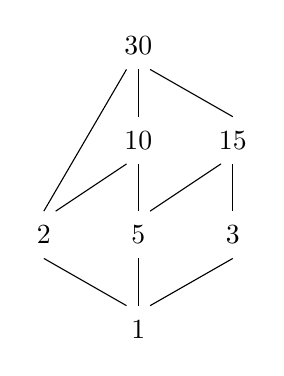
\begin{tikzpicture}[scale=0.6] %Replaced figure with tikz figure - TWJ 8/22/2010

\draw (0,0.5) -- (0,1.5);
\draw (0,2.5) -- (0,3.5);
\draw (2,2.5) -- (2,3.5);
\draw (0,4.5) -- (0,5.5);

\draw (0.25,5.5) -- (2,4.5);
\draw (-0.25,5.5) -- (-2,2.5);

\draw (1.75,3.5) -- (0.25,2.5);
\draw (-0.25,3.5) -- (-1.75,2.5);

\draw (2,1.5) -- (0.25,0.5);
\draw (-2,1.5) -- (-0.25,0.5);

\node at (0,6) {30};
\node at (0,4) {10};
\node at (2,4) {15};
\node at (-2, 2) {2};
\node at (0, 2) {5};
\node at (2, 2) {3};
\node at (0, 0) {1};

\end{tikzpicture}
\end{center}
 
 
 
\item[5.] 
False.
 

 
\item[6.]
(a) $(a \vee b \vee a') \wedge a$.
\begin{center}  
\tikzpreface{solution_circuit_a}
\begin{tikzpicture}[scale=0.8,node distance=5mm, text height=1.5ex,text depth=.25ex] %Replaced figure with tikz figure - TWJ 8/22/2010

\draw  (0,0) -- (2.2,0) (2.8,0) -- (4.7,0)  (5.3,0) -- (6,0);
\draw  (1,0) -- (1,1) -- (2.2,1)  (2.8,1) -- (4,1) -- (4,0);
\draw  (1,0) -- (1,-1) -- (2.2,-1)  (2.8,-1) -- (4,-1) -- (4,0);

\node at (2.5,-1) {$a'$};
\node at (2.5,0) {$b$};
\node at (2.5,1) {$a$};
\node at (5,0) {$a$};



\end{tikzpicture}
\end{center}
 


(c) $a \vee (a \wedge b)$.
\begin{center}  

\tikzpreface{solution_circuit_c}
\begin{tikzpicture}[scale=0.8,node distance=5mm, text height=1.5ex,text depth=.25ex] %Replaced figure with tikz figure - TWJ 8/22/2010

\draw  (0,0) -- (1,0) (4,0) -- (5,0);
\draw  (1,0) -- (1,1) -- (1.7,1)  (2.3,1) -- (2.7,1)  (3.3,1) -- (4,1) -- (4,0);
\draw  (1,0) -- (1,-1) -- (2.2,-1)  (2.8,-1) -- (4,-1) -- (4,0);

\node at (2.5,-1) {$a$};
\node at (2,1) {$a$};
\node at (3,1) {$b$};



\end{tikzpicture}
\end{center}
 
 
 
 
\item[8.]
Not equivalent.
 
\item[10.]
$a' \wedge [(a \wedge b') \vee b] = a \wedge (a \vee b)$.

\item[15.]
Let $I, J$ be ideals in $R$. We need to show that $I + J 
= \{ r + s : r \in
I \mbox{ and } s \in J  \}$ is the smallest ideal in $R$ containing
both $I$ and $J$. If $r_1, r_2 \in I$ and $s_1, s_2 \in J$, then
$(r_1 + s_1) + (r_2 + s_2) = (r_1 + r_2) +(s_1 + s_2)$ is in $I + J$.
For $a \in R$, $a(r_1 + s_1) = ar_1 + as_1 \in I + J$; hence, $I + J$
is an ideal in $R$.


\item[19.]
(a) No.

\item[21.]
$( \Rightarrow)$. $a = b \Rightarrow (a \wedge b') \vee (a' \wedge b)
= (a \wedge a') \vee (a' \wedge a) = O \vee O = O$. \\
$( \Leftarrow)$. $( a \wedge b') \vee (	a' \wedge b) = O \Rightarrow
a \vee b = (a \vee a) \vee b = a \vee (a \vee b) = a \vee [I \wedge
(a \vee b)] = a \vee [(a \vee a') \wedge (a \vee b)] = [a \vee
(a \wedge b')] \vee [a \vee (a' \wedge b)] = a \vee [(a \wedge b') \vee
(a' \wedge b)] = a \vee 0 = a$.  A symmetric argument shows that $a
\vee b = b$.



 
\end{itemize}
}
 
\subsection*{Chapter 20. Vector Spaces}
 
{\small
\begin{itemize}
 
\item[3.] 
${\mathbb Q}(\sqrt{2}, \sqrt{3}\, )$ has basis $\{ 1, \sqrt{2}, \sqrt{3},
\sqrt{6}\, \}$  over ${\mathbb Q}$.
 
\item[5.]
$P_n$ has basis $\{ 1, x, x^2, \ldots, x^{n-1} \}$.
 
\item[7.]
(a) Subspace of dimension 2 with basis $\{(1, 0, -3), (0, 1,
2) \}$.\\
(d) Not a subspace.
 
\item[10.]
$0 =  \alpha 0 = \alpha(-v+v) = \alpha(-v) + \alpha v \Rightarrow 
-\alpha v = \alpha(-v)$.
 
\item[12.]
Let $v_0 = 0, v_1, \ldots, v_n \in V$ and $\alpha_0 \neq 0, \alpha_1,
\ldots, \alpha_n \in F$. Then $\alpha_0 v_0 + \cdots + \alpha_n v_n =
0$.
 
\item[15.]
(a)
Let $u, v \in \ker(T)$ and $\alpha \in F$.  Then
\[
\begin{array}{c}
T(u +v) = T(u) + T(v) = 0 \\
T(\alpha v) = \alpha T(v) = \alpha 0 = 0.
\end{array}
\]
Hence, $u + v, \alpha v \in \ker(T) \Rightarrow \ker(T)$ is 
a subspace of
$V$. \\
(c) 
$T(u) = T(v) \Leftrightarrow T(u-v) = T(u) - T(v) = 0
\Leftrightarrow u-v = 0 \Leftrightarrow u = v$.
 
 
\item[17.]
(a)
Let $u, u' \in U$ and $v, v' \in V$. Then
\[
\begin{array}{c}
(u + v) + (u' + v') = (u + u') + (v + v') \in U + V \\
\alpha(u + v) = \alpha u + \alpha v \in U + V.
\end{array}
\]
 
\end{itemize}
}
 
\subsection*{Chapter 21. Fields}
 
{\small
\begin{itemize}
 
\item[1.] 
(a) $x^4 -\frac{2}{3} x^2 - \frac{62}{9}$.
(c) $x^4 - 2 x^2 + 25$.
 
\item[2.] 
(a) $\{ 1, \sqrt{2}, \sqrt{3}, \sqrt{6}\, \}$.
(c) $\{ 1, i, \sqrt{2}, \sqrt{2}\, i \}$.
(e) $\{1, 2^{1/6}, 2^{1/3}, 2^{1/2}, 2^{2/3}, 2^{5/6}  \}$.
 
\item[3.]
(a) ${\mathbb Q}(\sqrt{3}, \sqrt{7}\, )$.
 

\item[5.]
Use the fact that the elements of ${\mathbb Z}_2[x]/ \langle x^3 + x +
1\rangle$ are 0, 1, $\alpha$, $1 + \alpha$, $\alpha^2$, $1 + \alpha^2$,
$\alpha + \alpha^2$, $1 + \alpha + \alpha^2$ and the fact that
$\alpha^3 + \alpha + 1 = 0$. 


\item[8.]
False.


\item[14.]
Suppose that $E$ is algebraic over $F$ and $K$ is
algebraic over $E$. Let $\alpha \in K$. It suffices to show that
$\alpha$ is algebraic over some finite extension of $F$. Since
$\alpha$ is algebraic over $E$, it must be the zero of some polynomial
$p(x) = \beta_0 + \beta_1 x + \cdots + \beta_n x^n$ in $E[x]$. Hence
$\alpha$ is algebraic over $F(\beta_0, \ldots, \beta_n)$.


\item[22.]
${\mathbb Q}( \sqrt{3}, \sqrt{7}\, ) \supset {\mathbb Q}( \sqrt{3} +\sqrt{7}\,
)$ since $\{ 1, \sqrt{3}, \sqrt{7}, \sqrt{21}\, \}$ is a basis for
${\mathbb Q}( \sqrt{3}, \sqrt{7}\, )$ over ${\mathbb Q}$. Since $[{\mathbb Q}(
\sqrt{3}, \sqrt{7}\, ) : {\mathbb Q}] = 4$, $[{\mathbb Q}( \sqrt{3}
+\sqrt{7}\, ) : {\mathbb Q}] = 2$ or 4. Since the degree of the minimal
polynomial of $\sqrt{3} +\sqrt{7}$ is 4, ${\mathbb Q}( \sqrt{3},
\sqrt{7}\, ) = {\mathbb Q}( \sqrt{3} +\sqrt{7}\, )$.


\item[27.]
Let $\beta \in F(\alpha)$ not in $F$. Then $\beta =
p(\alpha)/q(\alpha)$, where $p$ and $q$ are polynomials in $\alpha$
with $q(\alpha) \neq 0$ and coefficients in $F$. If $\beta$ is
algebraic over $F$, then there exists a polynomial $f(x) \in F[x]$
such that $f(\beta) = 0$. Let $f(x) = a_0 + a_1 x + \cdots + a_n x^n$.
Then  
\[
0 = f(\beta) = f\left( 
\frac{p(\alpha)}{q(\alpha)} \right)
= a_0 + a_1 \left( \frac{p(\alpha)}{q(\alpha)} \right)  + \cdots + a_n
\left( \frac{p(\alpha)}{q(\alpha)} \right)^n. 
\]
Now multiply both sides by $q(\alpha)^n$ to show that there is a
polynomial in $F[x]$ that has $\alpha$ as a zero.




\end{itemize}
}
 
\subsection*{Chapter 22. Finite Fields}
 
{\small
\begin{itemize}

\item[1.]
(a) 2.
(c) 2.
 
\item[4.] 
There are eight elements in ${\mathbb Z}_2(\alpha)$. Exhibit two more
zeros of $x^3 + x^2 + 1$ other than $\alpha$ in these eight elements. 
 
\item[5.] 
Find an irreducible polynomial $p(x)$ in ${\mathbb Z}_3[x]$ of degree
3 and show that ${\mathbb Z}_3[x]/ \langle p(x) \rangle$ has 27
elements. 

\item[7.]
(a) $x^5 -1 = (x+1)(x^4+x^3 + x^2 + x+ 1)$. \\
(c) $x^9 -1 = (x+1)( x^2 + x+ 1)(x^6+x^3+1)$.
 
\item[8.]
True.

\item[11.]
(a) Use the fact that $x^7 -1 = (x+1)( x^3 + x+ 1)(x^3+x^2+1)$.

\item[12.]
False.

\item[17.]
If $p(x) \in F[x]$, then $p(x) \in E[x]$.


\item[18.]
Since $\alpha$ is algebraic over $F$ of degree $n$, we can write any
element $\beta \in F(\alpha)$ uniquely as $\beta = a_0  + a_1 \alpha +
\cdots + a_{n-1} \alpha^{n-1}$ with $a_i \in F$. There are $q^n$
possible $n$-tuples $(a_0, a_1, \ldots, a_{n-1})$.


\item[24.]
Factor $x^{p-1} - 1$ over ${\mathbb Z}_p$.


\end{itemize}
}
 
\subsection*{Chapter 23. Galois Theory}
 
{\small
\begin{itemize}
 
\item[1.]
(a) ${\mathbb Z}_2$.
(c) ${\mathbb Z}_2 \times {\mathbb Z}_2 \times {\mathbb Z}_2$.
 
\item[2.]
(a) Separable.
(c) Not separable.
 
\item[3.]
$[{\rm GF}(729): {\rm GF}(9)] = [{\rm GF}(729): {\rm GF}(3)] /[{\rm
GF}(9): {\rm GF}(3)] = 6/2 = 3 \Rightarrow G({\rm GF}(729)/ {\rm
GF}(9)) \cong {\mathbb Z}_3$. A generator for $G({\rm GF}(729)/ {\rm
GF}(9))$ is $\sigma$, where $\sigma_{3^6}( \alpha) = \alpha^{3^6} =
\alpha^{729}$ for $\alpha \in {\rm GF}(729)$.

\item[4.]
(a) $S_5$.
(c) $S_3$.

\item[5.]
(a) ${\mathbb Q}(i)$.


\item[7.]
Let $E$ be the splitting field of a cubic polynomial in $F[x]$. Show that
\mbox{$[E:F]$} is less than or equal to 6 and is divisible by 3. Since $G(E/F)$ is a subgroup of
$S_3$ whose order is divisible by 3, conclude that this group must be 
isomorphic to ${\mathbb Z}_3$ or $S_3$.
 
\item[9.]
$G$ is a subgroup of $S_n$.

\item[16.]
True.

\item[20.]
(a) Clearly $\omega, \omega^2, \ldots, \omega^{p-1}$ are
distinct since $\omega \neq 1$ or 0. To show that $\omega^i$ is a zero
of $\Phi_p$, calculate $\Phi_p( \omega^i)$. \\
(b) The conjugates of $\omega$ are $\omega, \omega^2, \ldots,
\omega^{p-1}$. Define a map  $\phi_i: {\mathbb Q}(\omega)
\rightarrow {\mathbb Q}(\omega^i)$ by 
\[
\phi_i(a_0 + a_1 \omega +
\cdots + a_{p-2} \omega^{p-2}) = a_0 + a_1 \omega^i + \cdots + c_{p-2} 
(\omega^i)^{p-2},
\]
where $a_i \in {\mathbb Q}$. Prove that $\phi_i$ is an isomorphism of
fields. Show that $\phi_2$ 
generates $G({\mathbb Q}(\omega)/{\mathbb Q})$. \\ 
(c)
Show that $\{ \omega, \omega^2, \ldots, \omega^{p-1} \}$ is a basis
for ${\mathbb Q}( \omega )$ over ${\mathbb Q}$, and consider which linear
combinations of $\omega, \omega^2, \ldots, \omega^{p-1}$ are left
fixed by all elements of $G( {\mathbb Q}( \omega ) / {\mathbb Q})$.
 
 
 
\end{itemize}
}
 
 
 
 
\pagestyle{headings}
 
 
 
 

%% RAB, 2009/01/28
%% Include GFDL as an appendix
%%
{\small\include{gfdl}}

\clearpage\addcontentsline{toc}{chapter}{Index}
{\small\printindex}

%% RAB, 2009/01/28
%% Ditched endnotes for improved notation.tex
%%
%% %%%%(c)
%%%%(c)  This file is a portion of the source for the textbook
%%%%(c)
%%%%(c)    Abstract Algebra: Theory and Applications
%%%%(c)    Copyright 1997 by Thomas W. Judson
%%%%(c)
%%%%(c)  See the file COPYING.txt for copying conditions
%%%%(c)
%%%%(c)
%\chapter*{Notation}


\pagestyle{empty}




 { \parindent 0pt \centering% was \raggedright
 \hrule height .5pt\vspace{40pt}
 \huge \bf Notation\par
 \nobreak \vskip 40pt \framebox[\hsize]{\hspace*{1in}}}
 \vskip 36pt plus 12pt minus 6pt 




 
\begin{tabbing}
\hspace{1.9775in} \= \kill
{\bf Symbol}  \>  {\bf Description} \\
     \mbox{\hspace*{1in}} \\
$a \in A$ \>  $a$ is in the set $A$ \\
${\Bbb N}$ \>  the natural numbers \\
${\Bbb Z}$ \>  the integers \\
${\Bbb Q}$ \>  the rational numbers \\
${\Bbb R}$ \>  the real numbers \\
${\Bbb C}$ \>  the complex numbers \\
$A \subset B$ \>  $A$ is a subset of $B$ \\
$\emptyset$ \>  the empty set \\
$A \cup B$ \>  union of sets $A$ and $B$ \\
$A \cap B$ \>  intersection of sets $A$ and $B$ \\
$A'$ \>  complement of the  set $A$ \\
$A \setminus B$ \>  difference between sets $A$ and $B$ \\
$A \times B$ \>  Cartesian product of sets $A$ and $B$ \\
$A^n$ \>  $A \times \cdots \times A$ ($n$ times) \\
$id$ \>  identity mapping \\
$f^{-1}$ \>  inverse of the function $f$	\\
$a \equiv b \pmod{n}$ \>  $a$ is congruent to $b$ modulo $n$ \\
$n!$ \>  $n$ factorial \\
$\left(\begin{array}{c}n \\ k \end{array} \right)$ \>  binomial
     coefficient $n!/(k! (n-k)!)$ \\
$m \mid n$ \>  $m$ divides $n$ \\
$\gcd(m, n)$ \>  greatest common divisor of $m$ and $n$ \\
${\cal P}(X)$ \>  power set of $X$ \\
${\Bbb Z}_n$ \>  the integers modulo $n$ \\
\end{tabbing} \clearpage
\begin{tabbing}
\hspace{1.9775in} \= \kill
{\bf Symbol}  \>  {\bf Description} \\
     \mbox{\hspace*{1in}} \\
$\lcm(m,n)$ \>  least common multiple of $m$ and $n$ \\
$U(n)$ \>  group of units in ${\Bbb Z}_n$ \\
${\Bbb M}_n ( {\Bbb R})$ \>  the $n \times n$ matrices with entries in
     ${\Bbb R}$ \\
$\det A$ \>  determinant of $A$ \\
$GL_n({\Bbb R})$ \>  general linear group \\
$Q_8$ \>  the group of quaternions \\
${\Bbb C}^\ast$ \>  the multiplicative group of complex numbers \\
$|G|$ \>  order of a group $G$ \\
${\Bbb R}^*$ \>  the multiplicative group of real numbers \\
${\Bbb Q}^*$ \>  the multiplicative group of rational numbers \\
$SL_n({\Bbb R})$ \>  special linear group \\
$Z(G)$ \>  center of a group $G$ \\
$\langle a \rangle$ \>  cyclic subgroup generated by $a$ \\
$|a|$ \>  order of an element $a$ \\
$\cis \theta$ \>  $\cos \theta + i \sin \theta$ \\
${\Bbb T}$ \>  the circle group \\
$S_n$ \>  symmetric group on $n$ letters \\
$(a_1, a_2, \ldots, a_k )$ \>  cycle of length $k$ \\
$A_n$ \>  alternating group on $n$ letters \\
$D_n$ \>  dihedral group \\
$[G:H]$ \>  index of a subgroup $H$ in a group $G$ \\
${\cal L}_H$ \>  set of left cosets of $H$ in a group $G$ \\
${\cal R}_H$ \>  set of right cosets of $H$ in a group $G$ \\
$d({\bold x}, {\bold y})$ \>  Hamming distance between ${\bold x}$ and
     ${\bold y}$ \\
$d_{\min}$ \>  minimum distance of a code \\
$w({\bold x})$ \>  weight of ${\bold x}$ \\
${\Bbb M}_{m \times n}({\Bbb Z}_2)$ \>  set of $m$ by $n$ matrices with 
     entries in ${\Bbb Z}_2$ \\
${\rm Null}(H)$ \>  null space of a matrix $H$ \\
$\delta_{ij}$ \>  Kronecker delta \\
$G \cong H$ \>  $G$ is isomorphic to $H$ \\
$\aut(G)$ \>  automorphism group of $G$ \\
$i_g$ \>  $i_g(x) = gxg^{-1}$ \\
$\inn(G)$ \>  inner automorphism group of $G$ \\
$\rho_g$ \>  right regular representation \\
\end{tabbing} \clearpage
\begin{tabbing}
\hspace{1.9775in} \= \kill
{\bf Symbol}  \>  {\bf Description} \\
     \mbox{\hspace*{1in}} \\
$G/N$ \>  factor group of $G$ mod $N$ \\
$\ker \phi$ \>  kernel of $\phi$ \\
$G'$ \>  commutator subgroup of $G$ \\
$(a_{ij})$ \>  matrix \\
$O(n)$ \>  orthogonal group \\
$\| {\bold x} \|$ \>  length of a vector ${\bold x}$ \\
$SO(n)$ \>  special orthogonal group \\
$E(n)$ \>  Euclidean group \\
${\cal O}_x$ \>  orbit of $x$ \\
$X_g$ \>  fixed point set of $g$ \\
$G_x$ \>  isotropy subgroup of $x$ \\
$X_G$ \>  set of fixed points in a $G$-set $X$ \\
$N(H)$ \>  normalizer of a subgroup $H$ \\
${\Bbb H}$ \>  the ring of quaternions \\
\mbox{char$\, R$} \>  characteristic of a ring $R$ \\
${\Bbb Z}[i ]$ \>  the Gaussian integers \\
${\Bbb Z}_{(p)}$ \>  ring of integers localized at $p$ \\
$R[x]$ \>  ring of polynomials over $R$ \\
$\deg p(x)$ \>  degree of $p(x)$ \\
$R[x_1, x_2, \ldots, x_n]$ \>  ring of polynomials in $n$ variables \\
$\phi_{\alpha}$ \>  evaluation homomorphism at $\alpha$ \\
${\Bbb Q}(x)$ \>  field of rational functions over ${\Bbb Q}$ \\
$\nu(a)$ \>  Euclidean valuation of $a$ \\
$F(x)$ \>  field of rational functions in $x$ \\
$F(x_1, \ldots, x_n)$ \>  field of rational functions in 
     $x_1, \ldots, x_n$ \\
$a \preceq b$ \>   $a$ is less than $b$ \\
$a \wedge b$ \>  meet of $a$ and $b$ \\
$a \vee b$ \>  join of $a$ and $b$ \\
$I$ \>  largest element in a lattice \\
$O$ \>  smallest element in a lattice \\
$a'$ \>  complement of $a$ in a lattice \\
$\dim V$ \>  dimension of a vector space $V$ \\
$U \oplus V$ \>  direct sum of vector spaces $U$ and $V$ \\
$\mbox{Hom}(V, W)$ \>  set of all linear transformations from $U$ to
     $V$ \\  
\end{tabbing} \clearpage
\begin{tabbing}
\hspace{1.9775in} \=  \kill
{\bf Symbol}  \>  {\bf Description} \\
     \mbox{\hspace*{1.0in}} \\
$V^\ast$ \>  dual of a vector space $V$ \\
$F( \alpha_1, \ldots, \alpha_n)$ \>  smallest field containing $F$ and
     $\alpha_1, \ldots, \alpha_n$ \\
$[E:F]$ \>  dimension of a field extension of $E$ over $F$ \\
GF$(p^n)$ \>  Galois field of order $p^n$ \\
$F^*$ \>  multiplicative group of a field $F$ \\
$G(E/F)$ \>  Galois group of $E$ over $F$ \\
$F_{\{\sigma_i \}}$ \>  field fixed by automorphisms $\sigma_i$ \\
$F_G$ \>  field fixed by automorphism group $G$ \\
$\Delta^2$ \>  discriminant of a polynomial \\
\end{tabbing}
 
 
 
 

 
\end{document}
 
